
\documentclass[11.5pt,twoside]{article}
%%%%%%%%%%%%%%%%%%%%%%%%%%%%%%%%%%%%%%%%%%%%%%%%%%%%%%%%%%%%%%%%%%%%%%%%%%%%%%%%%%%%%%%%%%%%%%%%%%%%%%%%%%%%%%%%%%%%%%%%%%%%%%%%%%%%%%%%%%%%%%%%%%%%%%%%%%%%%%%%%%%%%%%%%%%%%%%%%%%%%%%%%%%%%%%%%%%%%%%%%%%%%%%%%%%%%%%%%%%%%%%%%%%%%%%%%%%%%%%%%%%%%%%%%%%%
\usepackage{chadstyle}

%TCIDATA{OutputFilter=Latex.dll}
%TCIDATA{Version=5.50.0.2960}
%TCIDATA{<META NAME="SaveForMode" CONTENT="1">}
%TCIDATA{BibliographyScheme=Manual}
%TCIDATA{LastRevised=Tuesday, April 15, 2014 12:00:45}
%TCIDATA{<META NAME="GraphicsSave" CONTENT="32">}

\newcommand{\proptitle}[1]{\color{ChadBlue} \textnormal{(#1):}}
\newtheorem{proposition}{\color{ChadGreen} Proposition}
\newcommand{\assume}[2]{{\bf{Assumption #1}} (#2)}
\newcommand{\clr}[1]{{\color{ChadBlue} #1}}
\newcommand{\clrg}[1]{{\color{ChadGreen} #1}}
\newcommand{\Proof}[2]{\newline {\hspace{-\parindent} {\color{ChadGreen}\bf Proof of Proposition}~\ref{#1}.}{\color{ChadBlue} #2} \vspace{.1in}}
\usepackage{amsfonts}
\usepackage{appendix}
\usepackage[pagewise,displaymath, mathlines]{lineno}
\usepackage{amssymb}
\usepackage{amsmath}
\usepackage{graphicx}
\usepackage{color}
\usepackage{refcount}
\usepackage{natbib}
\usepackage{bm}
\usepackage{hyperref}
\usepackage{epstopdf}
\setcounter{MaxMatrixCols}{10}
\newtheorem{theorem}{Theorem}
\newtheorem{acknowledgement}[theorem]{Acknowledgement}
\newtheorem{algorithm}[theorem]{Algorithm}
\newtheorem{assumption}{Assumption}
\newtheorem{axiom}{Axiom}
\newtheorem{case}[theorem]{Case}
\newtheorem{claim}[theorem]{Claim}
\newtheorem{conclusion}[theorem]{Conclusion}
\newtheorem{condition}[theorem]{Condition}
\newtheorem{conjecture}{Conjecture}
\newtheorem{corollary}{Corollary}
\newtheorem{criterion}[theorem]{Criterion}
\newtheorem{definition}{Definition}
\newtheorem{lemma}{Lemma}
\newtheorem{problem}[theorem]{Problem}
\newtheorem{solution}[theorem]{Solution}
\newtheorem{summary}[theorem]{Summary}
\newtheorem{example}{Example}
\newtheorem{exercise}{Exercise}
\newtheorem{notation}{Notation}
\newtheorem{remark}{Remark}
\newcommand{\bmat}{\begin{matrix}}
\newcommand{\emat}{\end{matrix}}
\newcommand{\ov}{\overline}
\newcommand{\un}{\underline}
\newcommand{\EE}{\mathbb E}
\newcommand{\var}{\mathrm{var}}
\newcommand{\cov}{\mathrm{cov}}
\newcommand{\corr}{\mathrm{corr}}
\newcommand{\dd}{\displaystyle}
\newcommand{\ZZ}{\mathbb{Z}}
\newcommand{\RR}{\mathbb{R}}
\newcommand{\FF}{\mathbb F}
\newcommand{\LL}{\mathbb L}
\newcommand{\MM}{\mathbb M}
\newcommand{\KK}{\mathbb K}
\newcommand{\HH}{\mathbb H}
\newcommand{\QQ}{\mathbb Q}
\newcommand{\CC}{\mathbb{C}}
\newcommand{\Pin}{P_{\text{in}}}
\newcommand{\bx}{\mathbf{x}}
\newcommand{\bp}{\mathbf{p}}
\newcommand{\by}{\mathbf{y}}
\newcommand{\cP}{{\cal P}}
\newcommand{\bB}{\mathbf B}
\newcommand{\bM}{\mathbf M}
\newcommand{\bS}{\mathbf S}
\newcommand{\phis}{\varphi}
\newcommand{\barphis}{\overline\phis}
\newcommand{\se}{\text{se}}
\newcommand{\daga}{a^\dagger}
\newcommand{\devides}{\bigl |}
\newcommand{\eval}{\biggl |}
\newcommand{\ybar}{\overline y}
\newcommand{\bWhat}{\hat{\mathbf W}}
\newcommand{\bW}{\mathbf W}
\newcommand{\bz}{\mathbf z}
\newcommand{\bs}{\mathbf s}
\newcommand{\rightas}{\stackrel{a.s.}{\rightarrow}}
\newcommand{\rightp}{\stackrel{p}{\rightarrow}}
\newcommand{\rightd}{\stackrel{d}{\rightarrow}}
\newcommand{\bI}{\mathbf I}
\newcommand{\barB}{{\overline B}}
\newcommand{\barC}{{\overline C}}
\newcommand{\pbar}{{\overline p}}
\newcommand{\bbar}{{\overline b}}
\newcommand{\mubar}{{\overline \mu}}

\newenvironment{proof}[1][Proof]{\noindent \textbf{#1.} }{\  \rule{0.5em}{0.5em}}
\topmargin=-1cm
\oddsidemargin=-0cm
\textheight=22.2cm
\textwidth=16cm
\setcounter{secnumdepth}{2}
\pagestyle{plain}
\setcounter{figure}{0}
%\setpagewiselinenumbers
%\linenumbers
% Macros for Scientific Word 3.5 documents saved with the LaTeX filter.
% Copyright (C) 2000 Mackichan Software, Inc.

\typeout{TCILATEX Macros for Scientific Word 3.5 <19 July 2000>.}
\typeout{NOTICE:  This macro file is NOT proprietary and may be 
freely copied and distributed.}
%
\makeatletter

%%%%%%%%%%%%%%%%%%%%%
% FMTeXButton
% This is used for putting TeXButtons in the 
% frontmatter of a document. Add a line like
% \QTagDef{FMTeXButton}{101}{} to the filter 
% section of the cst being used. Also add a
% new section containing:
%     [f_101]
%     ALIAS=FMTexButton
%     TAG_TYPE=FIELD
%     TAG_LEADIN=TeX Button:
%
% It also works to put \defs in the preamble after 
% the \input tcilatex
\def\FMTeXButton#1{#1}
%
%%%%%%%%%%%%%%%%%%%%%%
% macros for time
\newcount\@hour\newcount\@minute\chardef\@x10\chardef\@xv60
\def\tcitime{
\def\@time{%
  \@minute\time\@hour\@minute\divide\@hour\@xv
  \ifnum\@hour<\@x 0\fi\the\@hour:%
  \multiply\@hour\@xv\advance\@minute-\@hour
  \ifnum\@minute<\@x 0\fi\the\@minute
  }}%

%%%%%%%%%%%%%%%%%%%%%%
% macro for hyperref
%%% \@ifundefined{hyperref}{\def\hyperref#1#2#3#4{#2\ref{#4}#3}}{}

\def\x@hyperref#1#2#3{%
   % Trun off various catcodes before reading parameter 4
   \catcode`\~ = 12
   \catcode`\$ = 12
   \catcode`\_ = 12
   \catcode`\# = 12
   \catcode`\& = 12
   \y@hyperref{#1}{#2}{#3}%
}

\def\y@hyperref#1#2#3#4{%
   #2\ref{#4}#3
   \catcode`\~ = 13
   \catcode`\$ = 3
   \catcode`\_ = 8
   \catcode`\# = 6
   \catcode`\& = 4
}

\@ifundefined{hyperref}{\let\hyperref\x@hyperref}{}


% macro for external program call
\@ifundefined{qExtProgCall}{\def\qExtProgCall#1#2#3#4#5#6{\relax}}{}
%%%%%%%%%%%%%%%%%%%%%%
%
% macros for graphics
%
\def\FILENAME#1{#1}%
%
\def\QCTOpt[#1]#2{%
  \def\QCTOptB{#1}
  \def\QCTOptA{#2}
}
\def\QCTNOpt#1{%
  \def\QCTOptA{#1}
  \let\QCTOptB\empty
}
\def\Qct{%
  \@ifnextchar[{%
    \QCTOpt}{\QCTNOpt}
}
\def\QCBOpt[#1]#2{%
  \def\QCBOptB{#1}%
  \def\QCBOptA{#2}%
}
\def\QCBNOpt#1{%
  \def\QCBOptA{#1}%
  \let\QCBOptB\empty
}
\def\Qcb{%
  \@ifnextchar[{%
    \QCBOpt}{\QCBNOpt}%
}
\def\PrepCapArgs{%
  \ifx\QCBOptA\empty
    \ifx\QCTOptA\empty
      {}%
    \else
      \ifx\QCTOptB\empty
        {\QCTOptA}%
      \else
        [\QCTOptB]{\QCTOptA}%
      \fi
    \fi
  \else
    \ifx\QCBOptA\empty
      {}%
    \else
      \ifx\QCBOptB\empty
        {\QCBOptA}%
      \else
        [\QCBOptB]{\QCBOptA}%
      \fi
    \fi
  \fi
}
\newcount\GRAPHICSTYPE
%\GRAPHICSTYPE 0 is for TurboTeX
%\GRAPHICSTYPE 1 is for DVIWindo (PostScript)
%%%(removed)%\GRAPHICSTYPE 2 is for psfig (PostScript)
\GRAPHICSTYPE=\z@
\def\GRAPHICSPS#1{%
 \ifcase\GRAPHICSTYPE%\GRAPHICSTYPE=0
   \special{ps: #1}%
 \or%\GRAPHICSTYPE=1
   \special{language "PS", include "#1"}%
%%%\or%\GRAPHICSTYPE=2
%%%  #1%
 \fi
}%
%
\def\GRAPHICSHP#1{\special{include #1}}%
%
% \graffile{ body }                                  %#1
%          { contentswidth (scalar)  }               %#2
%          { contentsheight (scalar) }               %#3
%          { vertical shift when in-line (scalar) }  %#4

\def\graffile#1#2#3#4{%
%%% \ifnum\GRAPHICSTYPE=\tw@
%%%  %Following if using psfig
%%%  \@ifundefined{psfig}{\input psfig.tex}{}%
%%%  \psfig{file=#1, height=#3, width=#2}%
%%% \else
  %Following for all others
  % JCS - added BOXTHEFRAME, see below
    \bgroup
	   \@inlabelfalse
       \leavevmode
       \@ifundefined{bbl@deactivate}{\def~{\string~}}{\activesoff}%
        \raise -#4 \BOXTHEFRAME{%
           \hbox to #2{\raise #3\hbox to #2{\null #1\hfil}}}%
    \egroup
}%
%
% A box for drafts
\def\draftbox#1#2#3#4{%
 \leavevmode\raise -#4 \hbox{%
  \frame{\rlap{\protect\tiny #1}\hbox to #2%
   {\vrule height#3 width\z@ depth\z@\hfil}%
  }%
 }%
}%
%
\newcount\draft
\draft=\z@
\let\nographics=\draft
\newif\ifwasdraft
\wasdraftfalse

%  \GRAPHIC{ body }                                  %#1
%          { draft name }                            %#2
%          { contentswidth (scalar)  }               %#3
%          { contentsheight (scalar) }               %#4
%          { vertical shift when in-line (scalar) }  %#5
\def\GRAPHIC#1#2#3#4#5{%
   \ifnum\draft=\@ne\draftbox{#2}{#3}{#4}{#5}%
   \else\graffile{#1}{#3}{#4}{#5}%
   \fi
}
%
\def\addtoLaTeXparams#1{%
    \edef\LaTeXparams{\LaTeXparams #1}}%
%
% JCS -  added a switch BoxFrame that can 
% be set by including X in the frame params.
% If set a box is drawn around the frame.

\newif\ifBoxFrame \BoxFramefalse
\newif\ifOverFrame \OverFramefalse
\newif\ifUnderFrame \UnderFramefalse

\def\BOXTHEFRAME#1{%
   \hbox{%
      \ifBoxFrame
         \frame{#1}%
      \else
         {#1}%
      \fi
   }%
}


\def\doFRAMEparams#1{\BoxFramefalse\OverFramefalse\UnderFramefalse\readFRAMEparams#1\end}%
\def\readFRAMEparams#1{%
 \ifx#1\end%
  \let\next=\relax
  \else
  \ifx#1i\dispkind=\z@\fi
  \ifx#1d\dispkind=\@ne\fi
  \ifx#1f\dispkind=\tw@\fi
  \ifx#1t\addtoLaTeXparams{t}\fi
  \ifx#1b\addtoLaTeXparams{b}\fi
  \ifx#1p\addtoLaTeXparams{p}\fi
  \ifx#1h\addtoLaTeXparams{h}\fi
  \ifx#1X\BoxFrametrue\fi
  \ifx#1O\OverFrametrue\fi
  \ifx#1U\UnderFrametrue\fi
  \ifx#1w
    \ifnum\draft=1\wasdrafttrue\else\wasdraftfalse\fi
    \draft=\@ne
  \fi
  \let\next=\readFRAMEparams
  \fi
 \next
 }%
%
%Macro for In-line graphics object
%   \IFRAME{ contentswidth (scalar)  }               %#1
%          { contentsheight (scalar) }               %#2
%          { vertical shift when in-line (scalar) }  %#3
%          { draft name }                            %#4
%          { body }                                  %#5
%          { caption}                                %#6


\def\IFRAME#1#2#3#4#5#6{%
      \bgroup
      \let\QCTOptA\empty
      \let\QCTOptB\empty
      \let\QCBOptA\empty
      \let\QCBOptB\empty
      #6%
      \parindent=0pt
      \leftskip=0pt
      \rightskip=0pt
      \setbox0=\hbox{\QCBOptA}%
      \@tempdima=#1\relax
      \ifOverFrame
          % Do this later
          \typeout{This is not implemented yet}%
          \show\HELP
      \else
         \ifdim\wd0>\@tempdima
            \advance\@tempdima by \@tempdima
            \ifdim\wd0 >\@tempdima
               \setbox1 =\vbox{%
                  \unskip\hbox to \@tempdima{\hfill\GRAPHIC{#5}{#4}{#1}{#2}{#3}\hfill}%
                  \unskip\hbox to \@tempdima{\parbox[b]{\@tempdima}{\QCBOptA}}%
               }%
               \wd1=\@tempdima
            \else
               \textwidth=\wd0
               \setbox1 =\vbox{%
                 \noindent\hbox to \wd0{\hfill\GRAPHIC{#5}{#4}{#1}{#2}{#3}\hfill}\\%
                 \noindent\hbox{\QCBOptA}%
               }%
               \wd1=\wd0
            \fi
         \else
            \ifdim\wd0>0pt
              \hsize=\@tempdima
              \setbox1=\vbox{%
                \unskip\GRAPHIC{#5}{#4}{#1}{#2}{0pt}%
                \break
                \unskip\hbox to \@tempdima{\hfill \QCBOptA\hfill}%
              }%
              \wd1=\@tempdima
           \else
              \hsize=\@tempdima
              \setbox1=\vbox{%
                \unskip\GRAPHIC{#5}{#4}{#1}{#2}{0pt}%
              }%
              \wd1=\@tempdima
           \fi
         \fi
         \@tempdimb=\ht1
         %\advance\@tempdimb by \dp1
         \advance\@tempdimb by -#2
         \advance\@tempdimb by #3
         \leavevmode
         \raise -\@tempdimb \hbox{\box1}%
      \fi
      \egroup%
}%
%
%Macro for Display graphics object
%   \DFRAME{ contentswidth (scalar)  }               %#1
%          { contentsheight (scalar) }               %#2
%          { draft label }                           %#3
%          { name }                                  %#4
%          { caption}                                %#5
\def\DFRAME#1#2#3#4#5{%
 \begin{center}
     \let\QCTOptA\empty
     \let\QCTOptB\empty
     \let\QCBOptA\empty
     \let\QCBOptB\empty
	 \vbox\bgroup
        \ifOverFrame 
           #5\QCTOptA\par
        \fi
        \GRAPHIC{#4}{#3}{#1}{#2}{\z@}
        \ifUnderFrame 
           \par#5\QCBOptA
        \fi
	 \egroup
 \end{center}%
 }%
%
%Macro for Floating graphic object
%   \FFRAME{ framedata f|i tbph x F|T }              %#1
%          { contentswidth (scalar)  }               %#2
%          { contentsheight (scalar) }               %#3
%          { caption }                               %#4
%          { label }                                 %#5
%          { draft name }                            %#6
%          { body }                                  %#7
\def\FFRAME#1#2#3#4#5#6#7{%
 %If float.sty loaded and float option is 'h', change to 'H'  (gp) 1998/09/05
  \@ifundefined{floatstyle}
    {%floatstyle undefined (and float.sty not present), no change
     \begin{figure}[#1]%
    }
    {%floatstyle DEFINED
	 \ifx#1h%Only the h parameter, change to H
      \begin{figure}[H]%
	 \else
      \begin{figure}[#1]%
	 \fi
	}
  \let\QCTOptA\empty
  \let\QCTOptB\empty
  \let\QCBOptA\empty
  \let\QCBOptB\empty
  \ifOverFrame
    #4
    \ifx\QCTOptA\empty
    \else
      \ifx\QCTOptB\empty
        \caption{\QCTOptA}%
      \else
        \caption[\QCTOptB]{\QCTOptA}%
      \fi
    \fi
    \ifUnderFrame\else
      \label{#5}%
    \fi
  \else
    \UnderFrametrue%
  \fi
  \begin{center}\GRAPHIC{#7}{#6}{#2}{#3}{\z@}\end{center}%
  \ifUnderFrame
    #4
    \ifx\QCBOptA\empty
      \caption{}%
    \else
      \ifx\QCBOptB\empty
        \caption{\QCBOptA}%
      \else
        \caption[\QCBOptB]{\QCBOptA}%
      \fi
    \fi
    \label{#5}%
  \fi
  \end{figure}%
 }%
%
%
%    \FRAME{ framedata f|i tbph x F|T }              %#1
%          { contentswidth (scalar)  }               %#2
%          { contentsheight (scalar) }               %#3
%          { vertical shift when in-line (scalar) }  %#4
%          { caption }                               %#5
%          { label }                                 %#6
%          { name }                                  %#7
%          { body }                                  %#8
%
%    framedata is a string which can contain the following
%    characters: idftbphxFT
%    Their meaning is as follows:
%             i, d or f : in-line, display, or floating
%             t,b,p,h   : LaTeX floating placement options
%             x         : fit contents box to contents
%             F or T    : Figure or Table. 
%                         Later this can expand
%                         to a more general float class.
%
%
\newcount\dispkind%

\def\makeactives{
  \catcode`\"=\active
  \catcode`\;=\active
  \catcode`\:=\active
  \catcode`\'=\active
  \catcode`\~=\active
}
\bgroup
   \makeactives
   \gdef\activesoff{%
      \def"{\string"}
      \def;{\string;}
      \def:{\string:}
      \def'{\string'}
      \def~{\string~}
      %\bbl@deactivate{"}%
      %\bbl@deactivate{;}%
      %\bbl@deactivate{:}%
      %\bbl@deactivate{'}%
    }
\egroup

\def\FRAME#1#2#3#4#5#6#7#8{%
 \bgroup
 \ifnum\draft=\@ne
   \wasdrafttrue
 \else
   \wasdraftfalse%
 \fi
 \def\LaTeXparams{}%
 \dispkind=\z@
 \def\LaTeXparams{}%
 \doFRAMEparams{#1}%
 \ifnum\dispkind=\z@\IFRAME{#2}{#3}{#4}{#7}{#8}{#5}\else
  \ifnum\dispkind=\@ne\DFRAME{#2}{#3}{#7}{#8}{#5}\else
   \ifnum\dispkind=\tw@
    \edef\@tempa{\noexpand\FFRAME{\LaTeXparams}}%
    \@tempa{#2}{#3}{#5}{#6}{#7}{#8}%
    \fi
   \fi
  \fi
  \ifwasdraft\draft=1\else\draft=0\fi{}%
  \egroup
 }%
%
% This macro added to let SW gobble a parameter that
% should not be passed on and expanded. 

\def\TEXUX#1{"texux"}

%
% Macros for text attributes:
%
\def\BF#1{{\bf {#1}}}%
\def\NEG#1{\leavevmode\hbox{\rlap{\thinspace/}{$#1$}}}%
%
%%%%%%%%%%%%%%%%%%%%%%%%%%%%%%%%%%%%%%%%%%%%%%%%%%%%%%%%%%%%%%%%%%%%%%%%
%
%
% macros for user - defined functions
\def\limfunc#1{\mathop{\rm #1}}%
\def\func#1{\mathop{\rm #1}\nolimits}%
% macro for unit names
\def\unit#1{\mathop{\rm #1}\nolimits}%

%
% miscellaneous 
\long\def\QQQ#1#2{%
     \long\expandafter\def\csname#1\endcsname{#2}}%
\@ifundefined{QTP}{\def\QTP#1{}}{}
\@ifundefined{QEXCLUDE}{\def\QEXCLUDE#1{}}{}
\@ifundefined{Qlb}{\def\Qlb#1{#1}}{}
\@ifundefined{Qlt}{\def\Qlt#1{#1}}{}
\def\QWE{}%
\long\def\QQA#1#2{}%
\def\QTR#1#2{{\csname#1\endcsname #2}}%(gp) Is this the best?
\long\def\TeXButton#1#2{#2}%
\long\def\QSubDoc#1#2{#2}%
\def\EXPAND#1[#2]#3{}%
\def\NOEXPAND#1[#2]#3{}%
\def\PROTECTED{}%
\def\LaTeXparent#1{}%
\def\ChildStyles#1{}%
\def\ChildDefaults#1{}%
\def\QTagDef#1#2#3{}%

% Constructs added with Scientific Notebook
\@ifundefined{correctchoice}{\def\correctchoice{\relax}}{}
\@ifundefined{HTML}{\def\HTML#1{\relax}}{}
\@ifundefined{TCIIcon}{\def\TCIIcon#1#2#3#4{\relax}}{}
\if@compatibility
  \typeout{Not defining UNICODE  U or CustomNote commands for LaTeX 2.09.}
\else
  \providecommand{\UNICODE}[2][]{\protect\rule{.1in}{.1in}}
  \providecommand{\U}[1]{\protect\rule{.1in}{.1in}}
  \providecommand{\CustomNote}[3][]{\marginpar{#3}}
\fi

%
% Macros for style editor docs
\@ifundefined{StyleEditBeginDoc}{\def\StyleEditBeginDoc{\relax}}{}
%
% Macros for footnotes
\def\QQfnmark#1{\footnotemark}
\def\QQfntext#1#2{\addtocounter{footnote}{#1}\footnotetext{#2}}
%
% Macros for indexing.
%
\@ifundefined{TCIMAKEINDEX}{}{\makeindex}%
%
% Attempts to avoid problems with other styles
\@ifundefined{abstract}{%
 \def\abstract{%
  \if@twocolumn
   \section*{Abstract (Not appropriate in this style!)}%
   \else \small 
   \begin{center}{\bf Abstract\vspace{-.5em}\vspace{\z@}}\end{center}%
   \quotation 
   \fi
  }%
 }{%
 }%
\@ifundefined{endabstract}{\def\endabstract
  {\if@twocolumn\else\endquotation\fi}}{}%
\@ifundefined{maketitle}{\def\maketitle#1{}}{}%
\@ifundefined{affiliation}{\def\affiliation#1{}}{}%
\@ifundefined{proof}{\def\proof{\noindent{\bfseries Proof. }}}{}%
\@ifundefined{endproof}{\def\endproof{\mbox{\ \rule{.1in}{.1in}}}}{}%
\@ifundefined{newfield}{\def\newfield#1#2{}}{}%
\@ifundefined{chapter}{\def\chapter#1{\par(Chapter head:)#1\par }%
 \newcount\c@chapter}{}%
\@ifundefined{part}{\def\part#1{\par(Part head:)#1\par }}{}%
\@ifundefined{section}{\def\section#1{\par(Section head:)#1\par }}{}%
\@ifundefined{subsection}{\def\subsection#1%
 {\par(Subsection head:)#1\par }}{}%
\@ifundefined{subsubsection}{\def\subsubsection#1%
 {\par(Subsubsection head:)#1\par }}{}%
\@ifundefined{paragraph}{\def\paragraph#1%
 {\par(Subsubsubsection head:)#1\par }}{}%
\@ifundefined{subparagraph}{\def\subparagraph#1%
 {\par(Subsubsubsubsection head:)#1\par }}{}%
%%%%%%%%%%%%%%%%%%%%%%%%%%%%%%%%%%%%%%%%%%%%%%%%%%%%%%%%%%%%%%%%%%%%%%%%
% These symbols are not recognized by LaTeX
\@ifundefined{therefore}{\def\therefore{}}{}%
\@ifundefined{backepsilon}{\def\backepsilon{}}{}%
\@ifundefined{yen}{\def\yen{\hbox{\rm\rlap=Y}}}{}%
\@ifundefined{registered}{%
   \def\registered{\relax\ifmmode{}\r@gistered
                    \else$\m@th\r@gistered$\fi}%
 \def\r@gistered{^{\ooalign
  {\hfil\raise.07ex\hbox{$\scriptstyle\rm\text{R}$}\hfil\crcr
  \mathhexbox20D}}}}{}%
\@ifundefined{Eth}{\def\Eth{}}{}%
\@ifundefined{eth}{\def\eth{}}{}%
\@ifundefined{Thorn}{\def\Thorn{}}{}%
\@ifundefined{thorn}{\def\thorn{}}{}%
% A macro to allow any symbol that requires math to appear in text
\def\TEXTsymbol#1{\mbox{$#1$}}%
\@ifundefined{degree}{\def\degree{{}^{\circ}}}{}%
%
% macros for T3TeX files
\newdimen\theight
\@ifundefined{Column}{\def\Column{%
 \vadjust{\setbox\z@=\hbox{\scriptsize\quad\quad tcol}%
  \theight=\ht\z@\advance\theight by \dp\z@\advance\theight by \lineskip
  \kern -\theight \vbox to \theight{%
   \rightline{\rlap{\box\z@}}%
   \vss
   }%
  }%
 }}{}%
%
\@ifundefined{qed}{\def\qed{%
 \ifhmode\unskip\nobreak\fi\ifmmode\ifinner\else\hskip5\p@\fi\fi
 \hbox{\hskip5\p@\vrule width4\p@ height6\p@ depth1.5\p@\hskip\p@}%
 }}{}%
%
\@ifundefined{cents}{\def\cents{\hbox{\rm\rlap/c}}}{}%
\@ifundefined{miss}{\def\miss{\hbox{\vrule height2\p@ width 2\p@ depth\z@}}}{}%
%
\@ifundefined{vvert}{\def\vvert{\Vert}}{}%  %always translated to \left| or \right|
%
\@ifundefined{tcol}{\def\tcol#1{{\baselineskip=6\p@ \vcenter{#1}} \Column}}{}%
%
\@ifundefined{dB}{\def\dB{\hbox{{}}}}{}%        %dummy entry in column 
\@ifundefined{mB}{\def\mB#1{\hbox{$#1$}}}{}%   %column entry
\@ifundefined{nB}{\def\nB#1{\hbox{#1}}}{}%     %column entry (not math)
%
\@ifundefined{note}{\def\note{$^{\dag}}}{}%
%
\def\newfmtname{LaTeX2e}
% No longer load latexsym.  This is now handled by SWP, which uses amsfonts if necessary
%
\ifx\fmtname\newfmtname
  \DeclareOldFontCommand{\rm}{\normalfont\rmfamily}{\mathrm}
  \DeclareOldFontCommand{\sf}{\normalfont\sffamily}{\mathsf}
  \DeclareOldFontCommand{\tt}{\normalfont\ttfamily}{\mathtt}
  \DeclareOldFontCommand{\bf}{\normalfont\bfseries}{\mathbf}
  \DeclareOldFontCommand{\it}{\normalfont\itshape}{\mathit}
  \DeclareOldFontCommand{\sl}{\normalfont\slshape}{\@nomath\sl}
  \DeclareOldFontCommand{\sc}{\normalfont\scshape}{\@nomath\sc}
\fi

%
% Greek bold macros
% Redefine all of the math symbols 
% which might be bolded	 - there are 
% probably others to add to this list

\def\alpha{{\Greekmath 010B}}%
\def\beta{{\Greekmath 010C}}%
\def\gamma{{\Greekmath 010D}}%
\def\delta{{\Greekmath 010E}}%
\def\epsilon{{\Greekmath 010F}}%
\def\zeta{{\Greekmath 0110}}%
\def\eta{{\Greekmath 0111}}%
\def\theta{{\Greekmath 0112}}%
\def\iota{{\Greekmath 0113}}%
\def\kappa{{\Greekmath 0114}}%
\def\lambda{{\Greekmath 0115}}%
\def\mu{{\Greekmath 0116}}%
\def\nu{{\Greekmath 0117}}%
\def\xi{{\Greekmath 0118}}%
\def\pi{{\Greekmath 0119}}%
\def\rho{{\Greekmath 011A}}%
\def\sigma{{\Greekmath 011B}}%
\def\tau{{\Greekmath 011C}}%
\def\upsilon{{\Greekmath 011D}}%
\def\phi{{\Greekmath 011E}}%
\def\chi{{\Greekmath 011F}}%
\def\psi{{\Greekmath 0120}}%
\def\omega{{\Greekmath 0121}}%
\def\varepsilon{{\Greekmath 0122}}%
\def\vartheta{{\Greekmath 0123}}%
\def\varpi{{\Greekmath 0124}}%
\def\varrho{{\Greekmath 0125}}%
\def\varsigma{{\Greekmath 0126}}%
\def\varphi{{\Greekmath 0127}}%

\def\nabla{{\Greekmath 0272}}
\def\FindBoldGroup{%
   {\setbox0=\hbox{$\mathbf{x\global\edef\theboldgroup{\the\mathgroup}}$}}%
}

\def\Greekmath#1#2#3#4{%
    \if@compatibility
        \ifnum\mathgroup=\symbold
           \mathchoice{\mbox{\boldmath$\displaystyle\mathchar"#1#2#3#4$}}%
                      {\mbox{\boldmath$\textstyle\mathchar"#1#2#3#4$}}%
                      {\mbox{\boldmath$\scriptstyle\mathchar"#1#2#3#4$}}%
                      {\mbox{\boldmath$\scriptscriptstyle\mathchar"#1#2#3#4$}}%
        \else
           \mathchar"#1#2#3#4% 
        \fi 
    \else 
        \FindBoldGroup
        \ifnum\mathgroup=\theboldgroup % For 2e
           \mathchoice{\mbox{\boldmath$\displaystyle\mathchar"#1#2#3#4$}}%
                      {\mbox{\boldmath$\textstyle\mathchar"#1#2#3#4$}}%
                      {\mbox{\boldmath$\scriptstyle\mathchar"#1#2#3#4$}}%
                      {\mbox{\boldmath$\scriptscriptstyle\mathchar"#1#2#3#4$}}%
        \else
           \mathchar"#1#2#3#4% 
        \fi     	    
	  \fi}

\newif\ifGreekBold  \GreekBoldfalse
\let\SAVEPBF=\pbf
\def\pbf{\GreekBoldtrue\SAVEPBF}%
%

\@ifundefined{theorem}{\newtheorem{theorem}{Theorem}}{}
\@ifundefined{lemma}{\newtheorem{lemma}[theorem]{Lemma}}{}
\@ifundefined{corollary}{\newtheorem{corollary}[theorem]{Corollary}}{}
\@ifundefined{conjecture}{\newtheorem{conjecture}[theorem]{Conjecture}}{}
\@ifundefined{proposition}{\newtheorem{proposition}[theorem]{Proposition}}{}
\@ifundefined{axiom}{\newtheorem{axiom}{Axiom}}{}
\@ifundefined{remark}{\newtheorem{remark}{Remark}}{}
\@ifundefined{example}{\newtheorem{example}{Example}}{}
\@ifundefined{exercise}{\newtheorem{exercise}{Exercise}}{}
\@ifundefined{definition}{\newtheorem{definition}{Definition}}{}


\@ifundefined{mathletters}{%
  %\def\theequation{\arabic{equation}}
  \newcounter{equationnumber}  
  \def\mathletters{%
     \addtocounter{equation}{1}
     \edef\@currentlabel{\theequation}%
     \setcounter{equationnumber}{\c@equation}
     \setcounter{equation}{0}%
     \edef\theequation{\@currentlabel\noexpand\alph{equation}}%
  }
  \def\endmathletters{%
     \setcounter{equation}{\value{equationnumber}}%
  }
}{}

%Logos
\@ifundefined{BibTeX}{%
    \def\BibTeX{{\rm B\kern-.05em{\sc i\kern-.025em b}\kern-.08em
                 T\kern-.1667em\lower.7ex\hbox{E}\kern-.125emX}}}{}%
\@ifundefined{AmS}%
    {\def\AmS{{\protect\usefont{OMS}{cmsy}{m}{n}%
                A\kern-.1667em\lower.5ex\hbox{M}\kern-.125emS}}}{}%
\@ifundefined{AmSTeX}{\def\AmSTeX{\protect\AmS-\protect\TeX\@}}{}%
%

% This macro is a fix to eqnarray
\def\@@eqncr{\let\@tempa\relax
    \ifcase\@eqcnt \def\@tempa{& & &}\or \def\@tempa{& &}%
      \else \def\@tempa{&}\fi
     \@tempa
     \if@eqnsw
        \iftag@
           \@taggnum
        \else
           \@eqnnum\stepcounter{equation}%
        \fi
     \fi
     \global\tag@false
     \global\@eqnswtrue
     \global\@eqcnt\z@\cr}


\def\TCItag{\@ifnextchar*{\@TCItagstar}{\@TCItag}}
\def\@TCItag#1{%
    \global\tag@true
    \global\def\@taggnum{(#1)}}
\def\@TCItagstar*#1{%
    \global\tag@true
    \global\def\@taggnum{#1}}
%
%%%%%%%%%%%%%%%%%%%%%%%%%%%%%%%%%%%%%%%%%%%%%%%%%%%%%%%%%%%%%%%%%%%%%
%
\def\tfrac#1#2{{\textstyle {#1 \over #2}}}%
\def\dfrac#1#2{{\displaystyle {#1 \over #2}}}%
\def\binom#1#2{{#1 \choose #2}}%
\def\tbinom#1#2{{\textstyle {#1 \choose #2}}}%
\def\dbinom#1#2{{\displaystyle {#1 \choose #2}}}%
\def\QATOP#1#2{{#1 \atop #2}}%
\def\QTATOP#1#2{{\textstyle {#1 \atop #2}}}%
\def\QDATOP#1#2{{\displaystyle {#1 \atop #2}}}%
\def\QABOVE#1#2#3{{#2 \above#1 #3}}%
\def\QTABOVE#1#2#3{{\textstyle {#2 \above#1 #3}}}%
\def\QDABOVE#1#2#3{{\displaystyle {#2 \above#1 #3}}}%
\def\QOVERD#1#2#3#4{{#3 \overwithdelims#1#2 #4}}%
\def\QTOVERD#1#2#3#4{{\textstyle {#3 \overwithdelims#1#2 #4}}}%
\def\QDOVERD#1#2#3#4{{\displaystyle {#3 \overwithdelims#1#2 #4}}}%
\def\QATOPD#1#2#3#4{{#3 \atopwithdelims#1#2 #4}}%
\def\QTATOPD#1#2#3#4{{\textstyle {#3 \atopwithdelims#1#2 #4}}}%
\def\QDATOPD#1#2#3#4{{\displaystyle {#3 \atopwithdelims#1#2 #4}}}%
\def\QABOVED#1#2#3#4#5{{#4 \abovewithdelims#1#2#3 #5}}%
\def\QTABOVED#1#2#3#4#5{{\textstyle 
   {#4 \abovewithdelims#1#2#3 #5}}}%
\def\QDABOVED#1#2#3#4#5{{\displaystyle 
   {#4 \abovewithdelims#1#2#3 #5}}}%
%
% Macros for text size operators:
%
\def\tint{\mathop{\textstyle \int}}%
\def\tiint{\mathop{\textstyle \iint }}%
\def\tiiint{\mathop{\textstyle \iiint }}%
\def\tiiiint{\mathop{\textstyle \iiiint }}%
\def\tidotsint{\mathop{\textstyle \idotsint }}%
\def\toint{\mathop{\textstyle \oint}}%
\def\tsum{\mathop{\textstyle \sum }}%
\def\tprod{\mathop{\textstyle \prod }}%
\def\tbigcap{\mathop{\textstyle \bigcap }}%
\def\tbigwedge{\mathop{\textstyle \bigwedge }}%
\def\tbigoplus{\mathop{\textstyle \bigoplus }}%
\def\tbigodot{\mathop{\textstyle \bigodot }}%
\def\tbigsqcup{\mathop{\textstyle \bigsqcup }}%
\def\tcoprod{\mathop{\textstyle \coprod }}%
\def\tbigcup{\mathop{\textstyle \bigcup }}%
\def\tbigvee{\mathop{\textstyle \bigvee }}%
\def\tbigotimes{\mathop{\textstyle \bigotimes }}%
\def\tbiguplus{\mathop{\textstyle \biguplus }}%
%
%
%Macros for display size operators:
%
\def\dint{\displaystyle \int}%
\def\diint{\displaystyle \iint}%
\def\diiint{\displaystyle \iiint}%
\def\diiiint{\mathop{\displaystyle \iiiint }}%
\def\didotsint{\mathop{\displaystyle \idotsint }}%
\def\doint{\mathop{\displaystyle \oint}}%
\def\dsum{\mathop{\displaystyle \sum }}%
\def\dprod{\mathop{\displaystyle \prod }}%
\def\dbigcap{\mathop{\displaystyle \bigcap }}%
\def\dbigwedge{\mathop{\displaystyle \bigwedge }}%
\def\dbigoplus{\mathop{\displaystyle \bigoplus }}%
\def\dbigodot{\mathop{\displaystyle \bigodot }}%
\def\dbigsqcup{\mathop{\displaystyle \bigsqcup }}%
\def\dcoprod{\mathop{\displaystyle \coprod }}%
\def\dbigcup{\mathop{\displaystyle \bigcup }}%
\def\dbigvee{\mathop{\displaystyle \bigvee }}%
\def\dbigotimes{\mathop{\displaystyle \bigotimes }}%
\def\dbiguplus{\mathop{\displaystyle \biguplus }}%

%%%%%%%%%%%%%%%%%%%%%%%%%%%%%%%%%%%%%%%%%%%%%%%%%%%%%%%%%%%%%%%%%%%%%%%
% NOTE: The rest of this file is read only if amstex has not been
% loaded.  This section is used to define amstex constructs in the
% event they have not been defined.
%
%


\def\ExitTCILatex{\makeatother\endinput}

\bgroup
\ifx\ds@amstex\relax
   \message{amstex already loaded}\aftergroup\ExitTCILatex
\else
   \@ifpackageloaded{amsmath}%
      {\message{amsmath already loaded}\aftergroup\ExitTCILatex}
      {}
   \@ifpackageloaded{amstex}%
      {\message{amstex already loaded}\aftergroup\ExitTCILatex}
      {}
   \@ifpackageloaded{amsgen}%
      {\message{amsgen already loaded}\aftergroup\ExitTCILatex}
      {}
\fi
\egroup


%%%%%%%%%%%%%%%%%%%%%%%%%%%%%%%%%%%%%%%%%%%%%%%%%%%%%%%%%%%%%%%%%%%%%%%%
%%
%
%
%  Macros to define some AMS LaTeX constructs when 
%  AMS LaTeX has not been loaded
% 
% These macros are copied from the AMS-TeX package for doing
% multiple integrals.
%
\typeout{TCILATEX defining AMS-like constructs}
\let\DOTSI\relax
\def\RIfM@{\relax\ifmmode}%
\def\FN@{\futurelet\next}%
\newcount\intno@
\def\iint{\DOTSI\intno@\tw@\FN@\ints@}%
\def\iiint{\DOTSI\intno@\thr@@\FN@\ints@}%
\def\iiiint{\DOTSI\intno@4 \FN@\ints@}%
\def\idotsint{\DOTSI\intno@\z@\FN@\ints@}%
\def\ints@{\findlimits@\ints@@}%
\newif\iflimtoken@
\newif\iflimits@
\def\findlimits@{\limtoken@true\ifx\next\limits\limits@true
 \else\ifx\next\nolimits\limits@false\else
 \limtoken@false\ifx\ilimits@\nolimits\limits@false\else
 \ifinner\limits@false\else\limits@true\fi\fi\fi\fi}%
\def\multint@{\int\ifnum\intno@=\z@\intdots@                          %1
 \else\intkern@\fi                                                    %2
 \ifnum\intno@>\tw@\int\intkern@\fi                                   %3
 \ifnum\intno@>\thr@@\int\intkern@\fi                                 %4
 \int}%                                                               %5
\def\multintlimits@{\intop\ifnum\intno@=\z@\intdots@\else\intkern@\fi
 \ifnum\intno@>\tw@\intop\intkern@\fi
 \ifnum\intno@>\thr@@\intop\intkern@\fi\intop}%
\def\intic@{%
    \mathchoice{\hskip.5em}{\hskip.4em}{\hskip.4em}{\hskip.4em}}%
\def\negintic@{\mathchoice
 {\hskip-.5em}{\hskip-.4em}{\hskip-.4em}{\hskip-.4em}}%
\def\ints@@{\iflimtoken@                                              %1
 \def\ints@@@{\iflimits@\negintic@
   \mathop{\intic@\multintlimits@}\limits                             %2
  \else\multint@\nolimits\fi                                          %3
  \eat@}%                                                             %4
 \else                                                                %5
 \def\ints@@@{\iflimits@\negintic@
  \mathop{\intic@\multintlimits@}\limits\else
  \multint@\nolimits\fi}\fi\ints@@@}%
\def\intkern@{\mathchoice{\!\!\!}{\!\!}{\!\!}{\!\!}}%
\def\plaincdots@{\mathinner{\cdotp\cdotp\cdotp}}%
\def\intdots@{\mathchoice{\plaincdots@}%
 {{\cdotp}\mkern1.5mu{\cdotp}\mkern1.5mu{\cdotp}}%
 {{\cdotp}\mkern1mu{\cdotp}\mkern1mu{\cdotp}}%
 {{\cdotp}\mkern1mu{\cdotp}\mkern1mu{\cdotp}}}%
%
%
%  These macros are for doing the AMS \text{} construct
%
\def\RIfM@{\relax\protect\ifmmode}
\def\text{\RIfM@\expandafter\text@\else\expandafter\mbox\fi}
\let\nfss@text\text
\def\text@#1{\mathchoice
   {\textdef@\displaystyle\f@size{#1}}%
   {\textdef@\textstyle\tf@size{\firstchoice@false #1}}%
   {\textdef@\textstyle\sf@size{\firstchoice@false #1}}%
   {\textdef@\textstyle \ssf@size{\firstchoice@false #1}}%
   \glb@settings}

\def\textdef@#1#2#3{\hbox{{%
                    \everymath{#1}%
                    \let\f@size#2\selectfont
                    #3}}}
\newif\iffirstchoice@
\firstchoice@true
%
%These are the AMS constructs for multiline limits.
%
\def\Let@{\relax\iffalse{\fi\let\\=\cr\iffalse}\fi}%
\def\vspace@{\def\vspace##1{\crcr\noalign{\vskip##1\relax}}}%
\def\multilimits@{\bgroup\vspace@\Let@
 \baselineskip\fontdimen10 \scriptfont\tw@
 \advance\baselineskip\fontdimen12 \scriptfont\tw@
 \lineskip\thr@@\fontdimen8 \scriptfont\thr@@
 \lineskiplimit\lineskip
 \vbox\bgroup\ialign\bgroup\hfil$\m@th\scriptstyle{##}$\hfil\crcr}%
\def\Sb{_\multilimits@}%
\def\endSb{\crcr\egroup\egroup\egroup}%
\def\Sp{^\multilimits@}%
\let\endSp\endSb
%
%
%These are AMS constructs for horizontal arrows
%
\newdimen\ex@
\ex@.2326ex
\def\rightarrowfill@#1{$#1\m@th\mathord-\mkern-6mu\cleaders
 \hbox{$#1\mkern-2mu\mathord-\mkern-2mu$}\hfill
 \mkern-6mu\mathord\rightarrow$}%
\def\leftarrowfill@#1{$#1\m@th\mathord\leftarrow\mkern-6mu\cleaders
 \hbox{$#1\mkern-2mu\mathord-\mkern-2mu$}\hfill\mkern-6mu\mathord-$}%
\def\leftrightarrowfill@#1{$#1\m@th\mathord\leftarrow
\mkern-6mu\cleaders
 \hbox{$#1\mkern-2mu\mathord-\mkern-2mu$}\hfill
 \mkern-6mu\mathord\rightarrow$}%
\def\overrightarrow{\mathpalette\overrightarrow@}%
\def\overrightarrow@#1#2{\vbox{\ialign{##\crcr\rightarrowfill@#1\crcr
 \noalign{\kern-\ex@\nointerlineskip}$\m@th\hfil#1#2\hfil$\crcr}}}%
\let\overarrow\overrightarrow
\def\overleftarrow{\mathpalette\overleftarrow@}%
\def\overleftarrow@#1#2{\vbox{\ialign{##\crcr\leftarrowfill@#1\crcr
 \noalign{\kern-\ex@\nointerlineskip}$\m@th\hfil#1#2\hfil$\crcr}}}%
\def\overleftrightarrow{\mathpalette\overleftrightarrow@}%
\def\overleftrightarrow@#1#2{\vbox{\ialign{##\crcr
   \leftrightarrowfill@#1\crcr
 \noalign{\kern-\ex@\nointerlineskip}$\m@th\hfil#1#2\hfil$\crcr}}}%
\def\underrightarrow{\mathpalette\underrightarrow@}%
\def\underrightarrow@#1#2{\vtop{\ialign{##\crcr$\m@th\hfil#1#2\hfil
  $\crcr\noalign{\nointerlineskip}\rightarrowfill@#1\crcr}}}%
\let\underarrow\underrightarrow
\def\underleftarrow{\mathpalette\underleftarrow@}%
\def\underleftarrow@#1#2{\vtop{\ialign{##\crcr$\m@th\hfil#1#2\hfil
  $\crcr\noalign{\nointerlineskip}\leftarrowfill@#1\crcr}}}%
\def\underleftrightarrow{\mathpalette\underleftrightarrow@}%
\def\underleftrightarrow@#1#2{\vtop{\ialign{##\crcr$\m@th
  \hfil#1#2\hfil$\crcr
 \noalign{\nointerlineskip}\leftrightarrowfill@#1\crcr}}}%
%%%%%%%%%%%%%%%%%%%%%

\def\qopnamewl@#1{\mathop{\operator@font#1}\nlimits@}
\let\nlimits@\displaylimits
\def\setboxz@h{\setbox\z@\hbox}


\def\varlim@#1#2{\mathop{\vtop{\ialign{##\crcr
 \hfil$#1\m@th\operator@font lim$\hfil\crcr
 \noalign{\nointerlineskip}#2#1\crcr
 \noalign{\nointerlineskip\kern-\ex@}\crcr}}}}

 \def\rightarrowfill@#1{\m@th\setboxz@h{$#1-$}\ht\z@\z@
  $#1\copy\z@\mkern-6mu\cleaders
  \hbox{$#1\mkern-2mu\box\z@\mkern-2mu$}\hfill
  \mkern-6mu\mathord\rightarrow$}
\def\leftarrowfill@#1{\m@th\setboxz@h{$#1-$}\ht\z@\z@
  $#1\mathord\leftarrow\mkern-6mu\cleaders
  \hbox{$#1\mkern-2mu\copy\z@\mkern-2mu$}\hfill
  \mkern-6mu\box\z@$}


\def\projlim{\qopnamewl@{proj\,lim}}
\def\injlim{\qopnamewl@{inj\,lim}}
\def\varinjlim{\mathpalette\varlim@\rightarrowfill@}
\def\varprojlim{\mathpalette\varlim@\leftarrowfill@}
\def\varliminf{\mathpalette\varliminf@{}}
\def\varliminf@#1{\mathop{\underline{\vrule\@depth.2\ex@\@width\z@
   \hbox{$#1\m@th\operator@font lim$}}}}
\def\varlimsup{\mathpalette\varlimsup@{}}
\def\varlimsup@#1{\mathop{\overline
  {\hbox{$#1\m@th\operator@font lim$}}}}

%
%Companion to stackrel
\def\stackunder#1#2{\mathrel{\mathop{#2}\limits_{#1}}}%
%
%
% These are AMS environments that will be defined to
% be verbatims if amstex has not actually been 
% loaded
%
%
\begingroup \catcode `|=0 \catcode `[= 1
\catcode`]=2 \catcode `\{=12 \catcode `\}=12
\catcode`\\=12 
|gdef|@alignverbatim#1\end{align}[#1|end[align]]
|gdef|@salignverbatim#1\end{align*}[#1|end[align*]]

|gdef|@alignatverbatim#1\end{alignat}[#1|end[alignat]]
|gdef|@salignatverbatim#1\end{alignat*}[#1|end[alignat*]]

|gdef|@xalignatverbatim#1\end{xalignat}[#1|end[xalignat]]
|gdef|@sxalignatverbatim#1\end{xalignat*}[#1|end[xalignat*]]

|gdef|@gatherverbatim#1\end{gather}[#1|end[gather]]
|gdef|@sgatherverbatim#1\end{gather*}[#1|end[gather*]]

|gdef|@gatherverbatim#1\end{gather}[#1|end[gather]]
|gdef|@sgatherverbatim#1\end{gather*}[#1|end[gather*]]


|gdef|@multilineverbatim#1\end{multiline}[#1|end[multiline]]
|gdef|@smultilineverbatim#1\end{multiline*}[#1|end[multiline*]]

|gdef|@arraxverbatim#1\end{arrax}[#1|end[arrax]]
|gdef|@sarraxverbatim#1\end{arrax*}[#1|end[arrax*]]

|gdef|@tabulaxverbatim#1\end{tabulax}[#1|end[tabulax]]
|gdef|@stabulaxverbatim#1\end{tabulax*}[#1|end[tabulax*]]


|endgroup
  

  
\def\align{\@verbatim \frenchspacing\@vobeyspaces \@alignverbatim
You are using the "align" environment in a style in which it is not defined.}
\let\endalign=\endtrivlist
 
\@namedef{align*}{\@verbatim\@salignverbatim
You are using the "align*" environment in a style in which it is not defined.}
\expandafter\let\csname endalign*\endcsname =\endtrivlist




\def\alignat{\@verbatim \frenchspacing\@vobeyspaces \@alignatverbatim
You are using the "alignat" environment in a style in which it is not defined.}
\let\endalignat=\endtrivlist
 
\@namedef{alignat*}{\@verbatim\@salignatverbatim
You are using the "alignat*" environment in a style in which it is not defined.}
\expandafter\let\csname endalignat*\endcsname =\endtrivlist




\def\xalignat{\@verbatim \frenchspacing\@vobeyspaces \@xalignatverbatim
You are using the "xalignat" environment in a style in which it is not defined.}
\let\endxalignat=\endtrivlist
 
\@namedef{xalignat*}{\@verbatim\@sxalignatverbatim
You are using the "xalignat*" environment in a style in which it is not defined.}
\expandafter\let\csname endxalignat*\endcsname =\endtrivlist




\def\gather{\@verbatim \frenchspacing\@vobeyspaces \@gatherverbatim
You are using the "gather" environment in a style in which it is not defined.}
\let\endgather=\endtrivlist
 
\@namedef{gather*}{\@verbatim\@sgatherverbatim
You are using the "gather*" environment in a style in which it is not defined.}
\expandafter\let\csname endgather*\endcsname =\endtrivlist


\def\multiline{\@verbatim \frenchspacing\@vobeyspaces \@multilineverbatim
You are using the "multiline" environment in a style in which it is not defined.}
\let\endmultiline=\endtrivlist
 
\@namedef{multiline*}{\@verbatim\@smultilineverbatim
You are using the "multiline*" environment in a style in which it is not defined.}
\expandafter\let\csname endmultiline*\endcsname =\endtrivlist


\def\arrax{\@verbatim \frenchspacing\@vobeyspaces \@arraxverbatim
You are using a type of "array" construct that is only allowed in AmS-LaTeX.}
\let\endarrax=\endtrivlist

\def\tabulax{\@verbatim \frenchspacing\@vobeyspaces \@tabulaxverbatim
You are using a type of "tabular" construct that is only allowed in AmS-LaTeX.}
\let\endtabulax=\endtrivlist

 
\@namedef{arrax*}{\@verbatim\@sarraxverbatim
You are using a type of "array*" construct that is only allowed in AmS-LaTeX.}
\expandafter\let\csname endarrax*\endcsname =\endtrivlist

\@namedef{tabulax*}{\@verbatim\@stabulaxverbatim
You are using a type of "tabular*" construct that is only allowed in AmS-LaTeX.}
\expandafter\let\csname endtabulax*\endcsname =\endtrivlist

% macro to simulate ams tag construct


% This macro is a fix to the equation environment
 \def\endequation{%
     \ifmmode\ifinner % FLEQN hack
      \iftag@
        \addtocounter{equation}{-1} % undo the increment made in the begin part
        $\hfil
           \displaywidth\linewidth\@taggnum\egroup \endtrivlist
        \global\tag@false
        \global\@ignoretrue   
      \else
        $\hfil
           \displaywidth\linewidth\@eqnnum\egroup \endtrivlist
        \global\tag@false
        \global\@ignoretrue 
      \fi
     \else   
      \iftag@
        \addtocounter{equation}{-1} % undo the increment made in the begin part
        \eqno \hbox{\@taggnum}
        \global\tag@false%
        $$\global\@ignoretrue
      \else
        \eqno \hbox{\@eqnnum}% $$ BRACE MATCHING HACK
        $$\global\@ignoretrue
      \fi
     \fi\fi
 } 

 \newif\iftag@ \tag@false
 
 \def\TCItag{\@ifnextchar*{\@TCItagstar}{\@TCItag}}
 \def\@TCItag#1{%
     \global\tag@true
     \global\def\@taggnum{(#1)}}
 \def\@TCItagstar*#1{%
     \global\tag@true
     \global\def\@taggnum{#1}}

  \@ifundefined{tag}{
     \def\tag{\@ifnextchar*{\@tagstar}{\@tag}}
     \def\@tag#1{%
         \global\tag@true
         \global\def\@taggnum{(#1)}}
     \def\@tagstar*#1{%
         \global\tag@true
         \global\def\@taggnum{#1}}
  }{}
% Do not add anything to the end of this file.  
% The last section of the file is loaded only if 
% amstex has not been.



\makeatother
\endinput


\begin{document}
\author{\textbf{Anmol Bhandari}\\apb296@nyu.edu \and \textbf{David Evans} \\ \texttt{dgevans@nyu.edu} \and \textbf{Mikhail Golosov}\\\texttt{golosov@princeton.edu} \and \textbf{Thomas J. Sargent} \\ \texttt{thomas.sargent@nyu.edu}
}
\title{\textbf{Taxes, debts,  and redistributions with aggregate shocks%
\thanks{%
We thank Mark Aguiar, Stefania Albanesi, Manuel Amador,  Andrew Atkeson, Marco Bassetto, V.V. Chari, Harold
L. Cole, Guy Laroque, Francesco Lippi, Robert E. Lucas, Jr., Ali Shourideh, Pierre Yared and seminar
participants at Bocconi, Chicago, EIEF, the Federal Reserve Bank of
Minneapolis, IES, Princeton, Stanford, UCL, Universidade Cat\'{o}lica, 2012
Minnesota macro conference, Monetary Policy Workshop NY Fed for helpful
comments.}}}
\date{November 2014}
\maketitle
\begin{center}
\textbf{Abstract} 
\end{center}

This paper studies how taxes and debt respond to aggregate shocks in the presence of incomplete markets and redistribution concerns. A planner sets a lump sum transfer and a linear tax on labor income  in an economy with heterogeneous agents, aggregate uncertainty, and markets restricted to a single asset whose payoffs can wary with aggregate states. Two forces shape long-run outcomes: the planner's desire to minimize the welfare costs of fluctuating transfers, which calls for a negative correlation between the distribution of net  assets and agents' skills; and the planner's desire to use fluctuations in the real interest rate to adjust for missing state-contingent securities. In a model parameterized to match stylized facts about  US booms and recessions, distributional concerns  mainly determine optimal policies over business cycle frequencies.  These features of optimal policy differ markedly from ones that emerge from  representative agent Ramsey models


\medskip


\bigskip
\noindent{\sc Key words: }Distorting taxes. Transfers. Redistribution.  Government debt.  Interest rate risk.

\noindent{\sc JEL codes:} E62,H21,H63
\thispagestyle{empty}\bigskip

\bigskip \newpage

\setcounter{page}{1}

\bigskip \baselineskip0.65cm


%\textcolor{green}{I have not edited the green part.
%\input BEGS_intro_Tom_1


% 
% 
% \begin{quote}
% \emph{If, indeed, the debt were distributed in exact proportion to the taxes
% to be paid so that every one should pay out in taxes as much as he received
% in interest, it would cease to be a burden.% The idea of such a distribution
% %has already been shown to be chimerical; and
% $\ldots$ if it were possible, there
% would be [no] need of incurring the debt. For if a man has money to loan the
% Government, he certainly has money to pay the Government what he owes it.
% %His share of the debt has been incurred solely because it is presumed that
% %he has no money to spare.
% }Simon \citet[p.85]{newcomb1865critical}
% \end{quote}



\section{Introduction}
\section{Environment\label{Sec: environment}}
Exogenous fundamentals of the economy are functions of a shock $s_{t}$ that follows an irreducible Markov process, where $s_{t}\in S$ and $S$ is a finite set. We let $s^{t}=\left(s_{0},...,s_{t}\right)$
denote a history of shocks with marginal densities denoted by $Pr(s^t)$. \footnote{To save on notation, mostly we use $z_{t}$ to denote a random variable
with a time $t$ conditional distribution that is a function of the
history $s^{t}$. Occasionally, we use the more explicit notion $z\left(s^{t}\right)$
to denote a realization at a particular history $s^{t}.$} 

There is a mass $n_{i}$ of a type $i\in I$ agent, with $\sum_{i=1}^{I}n_{i}=1.$ Types differ by their skills. Preferences of an agent of type $i$ over stochastic processes for consumption $\{c_{i,t}\}_{t}$ and labor supply $\{l_{i,t}\}_{t}$
are ordered by 

\begin{equation}
\mathbb{E}_{0}\sum_{t=0}^{\infty}\beta^{t}U^{i}\left(c_{i,t},l_{i,t}\right),\label{utility lifetime}
\end{equation}

where $\mathbb{E}_{t}$ is a mathematical expectations operator conditioned on time $t$ information and $\beta\in\left(0,1\right)$ is the time discount factor. %We assume that $l_{i}\in\left[0,\bar{l}_{i}\right]$ for some $\bar{l}_{i}<\infty.$
Results in section \ref{sec:Ricardian101} require no additional assumptions on $U^{i}$ like differentiability
or convexity,\footnote{Consequently our setup allows both extensive and intensive responses
of labor.} but results in later sections do.

An agent of type $i$ who supplies $l_{i}$ units of labor produces
$\theta_{i}\left(s_{t}\right)l_{i}$ units of output, where $\theta_{i}(s_{t})\in\Theta$
is a nonnegative state-dependent scalar. Feasible allocations satisfy
\begin{equation}
\label{eqn:feasiblity}
\sum_{i=1}^{I}n_{i}c_{i,t}+g_{t}=\sum_{i=1}^{I}\pi_{i}\theta_{i,t}l_{i,t},\label{feasibility goods}
\end{equation}

where $g_{t}$ denotes exogenous government expenditures in state
$s_{t}.$

A Ramsey planner's preferences over a vector of stochastic processes
for consumption and labor supply are ordered by 
\begin{equation}
\mathbb{E}_{0}\sum_{i=1}^{I}\omega_{i}\sum_{t=0}^{\infty}\beta^{t}U_{t}^{i}\left(c_{i,t},l_{i,t}\right),\label{govmt objective}
\end{equation}
where the Pareto weights satisfy $\omega_{i}\geq0,$ $\sum_{i=1}^{I}\omega_{i}=1$

The government and agents trade a single but possibly risky asset whose
time $t$ payoff $p_{t}$ is described by an $S\times S$ matrix $\mathbb{P}$
\[
p_{t}=\mathbb{P}(s_{t}|s_{t-1}),
\]
with the normalization that $\mathbb{E}_{t}p_{t+1}=1$. The payoff shocks are a parsimonious way to capture variations in holding period returns on portfolio of the government due inflation risk, interest rate risk (for longer maturity bonds) or defaults risk.

We assume that the government imposes an affine tax. We denote proportional labor taxes by $\tau$ and lump sump transfers by $T$. With this
the tax bill of an agent with wage earnings $l_{i,t}\theta_{i,t}$
is given by 
\[
-T_{t}+\tau_{t}\theta_{i,t}l_{i,t}.
\]
%We allow the government to choose a feasible sequence of transfers $%%\{T_{t}\} $.

We do not restrict the sign of $T_{t}$ at any $t$ or $s^{t}$. If for some type $i$, $\theta_{i,t}=0$, $b_{i,-1}=0$ and $U^{i}$ is defined only on $\mathcal{R}_{+}^{2}$, his budget constraint will
imply that the all allocations feasible for the planner have nonnegative present values of transfers, since transfers are the sole source of
a type $i$ agent's wealth and consumption.


Let $q_t= q_t(s^t)$ be the price of the single  asset at time $t$ and $R_{t}=\frac{p_t}{q_{t-1}}$  be the one period returns from holding the asset from $t-1$ to $t$. Under the affine tax system, agent $i$'s budget constraint at $t$ is%
\begin{equation}
c_{i,t}+b_{i,t}=\left( 1-\tau _{t}\right) \theta
_{i,t}l_{i,t}+R_{t}b_{i,t-1}+T_{t},  \label{agent bc affine}
\end{equation}

\noindent where $b_{i,t}$ denotes asset holdings of a type $i$ agent  at time $t\geq 0$. 

The government budget constraint is%

\begin{equation}
g_{t}+B_{t}=\tau _{t}\sum_{i=1}^{I}n_{i}\theta
_{i,t}l_{i,t}-T_{t}+R_{t}B_{t-1},  \label{govmt bc affine}
\end{equation}%
where $B_{t}$ denotes the government's assets at time $t$.

We assume that private agents and the government start with  assets $%
\{b_{i,-1}\}_{i=1}^{I}$ and $B_{-1}$, respectively.  Asset holdings
satisfy the market clearing condition%

\begin{equation}
\label{feasibility bonds}
\sum_{i=1}^{I}n _{i}b_{i,t}+B_{t}=0\text{ for all }t\geq -1.
\end{equation}%
%Since $B_{t}$ and all $b_{i,t}$ are bounded from below,  equation (\ref{feasibility bonds}) implies that they are also bounded from above.


Components of  competitive  equilibria are described below

\begin{definition}
\label{Def:components} An \emph{allocation} is a sequence $\left \{
c_{i,t},l_{i,t}\right \} _{i,t}$. An \emph{asset profile} is a sequence $\{
\left \{ b_{i,t}\right \} _{i},B_{t}\}_{t}$. A \emph{price system} is an
interest rate sequence $\{R_{t}\}_{t}$. A \emph{tax policy} is a sequence $%
\{ \tau _{t},T_{t}\}_{t}$.
\end{definition}
%
%We next define a competitive equilibrium. The key feature of that definition
%is that equilibria defined for a given initial assets $\left( \left\{
%b_{i,-1}\right\} _{i},B_{-1}\right) $ and we study the implications of the
%initial assets on the equilibrium allocations.


Representative agent models usually impose debt limits on the government. Section XX describes that in our setting with affine taxes and heterogeneous agents, competitive allocations only pin down net asset positions. Thus $\tilde{D}_t=-(B_t-b_{i,t})$ for some $i$ is comparable to the notion of \emph{public debt} and we will assume that it is bounded. As far the households we will impose natural debt limits. These typically depend on the tax and transfer policies adopted by the government.\footnote{An alternative is to use ad-hoc debt limits which are exogenous history contingent bounds for each agent. Appendix XX discusses how restricting attention to natural debt limits for the households only shrinks the set of allocations that can be implemented as competitive equilibria.} 

\begin{definition}
\label{Def: CE with affine taxes}For a given initial asset distribution $\left(
\left \{ b_{i,-1}\right
\} _{i},B_{-1}\right) $, a competitive
equilibrium with affine taxes is a sequence $\{ \left
\{
c_{i,t},l_{i,t},b_{i,t}\right \} _{i},B_{t},R_{t}\}_t$ and a tax policy $%
\left \{ \tau _{t},T_{t}\right
\} _{t},$ %such that the allocation and the
%private components $\left \{b_{i,t}\right \} _{t}$ of the asset profile
%$\left \{ c_{i,t},l_{i,t},b_{i,t}\right \} _{i,t}$
such that $\{ c_{i,t},l_{i,t},b_{i,t} \} _{i,t}$
maximize (\ref{utility lifetime})\ subject to (\ref{agent bc affine}) and
$\{b_{i,t}\}_{i,t}$ satisfies the borrowing limits; and
constraints (\ref{feasibility goods}), (\ref{govmt bc affine})\ and (\ref%
{feasibility bonds})\ are satisfied.
\end{definition}

%To rule out Ponzi schemes,we assume that $b_{i,t}$ must be bounded from below.  Generally these bounds can be constructed using natural debt limits (which are endogenous and depend on the tax, trasnfers policies) or adhoc limits that are some exogenous history contingent functions. For most of the paper we will focus on the natural limits which simplify our characterization but 


%\textcolor{blue}{Each initial asset distribution $\left( \left\{
%b_{i,-1}\right\} _{i},B_{-1}\right) $ is associated with a competitive equilibrium.
%We want to study the effects  of the initial asset distribution on optimal competitive
%equilibrium outcomes.}

%\textcolor{blue}{From Anmol : does the previous sentence belong here ?}

\smallskip Lastly we define optimal competitive equilibria.

\begin{definition}
\label{Def: optimal CE affine} Given $(\{b_{i,-1}\}_{i},B_{-1})$, an
optimal competitive equilibrium with affine taxes is a tax
policy $\left\{ \tau _{t}^{\ast },T_{t}^{\ast }\right\} _{t}$, an allocation
$ \left\{ c_{i,t}^{\ast },l_{i,t}^{\ast } \right\})_{i,t}$, an asset profile
$\left\{\left\{b_{i,t}^{\ast }\right\}
_{i},B_{t}^{\ast }\right\} _{t}$, and a price system $\left\{ R_{t}^{\ast
}\right\} _{t}$ such that (i) given $\left( \left\{ b_{i,-1}\right\}
_{i},B_{-1}\right) $, the tax policy,  %tax-transfer system $\left\{ \tau _{t}^{\ast
%},T_{t}^{\ast }\right\} _{t}$,
 the price system, %$\left\{ R_{t}^{\ast
%}\right\} _{t}$,
and the allocation %$\left\{ \left\{ c_{i,t}^{\ast
%},l_{i,t}^{\ast },b_{i,t}^{\ast }\right\} _{i},B_{t}^{\ast }\right\} _{t}$
constitute a competitive equilibrium, (ii) $B_t$ satisfies the borrowing constraints; and (iii) there is no other tax policy $%
\left\{ \tau _{t},T_{t}\right\} _{t}$ such that a competitive equilibrium
given $\left( \left\{ b_{i,-1}\right\} _{i},B_{-1}\right) $ and $\left\{
\tau _{t},T_{t}\right\} _{t}$ has a strictly higher value of (\ref{govmt
objective})$.$
\end{definition}

\smallskip We  call $\left \{ \tau _{t}^{\ast },T_{t}^{\ast }\right \}
_{t}$ an \textit{optimal tax policy}, $\{c_{i,t}^{\ast },l_{i,t}^{\ast
}\}_{i,t}$ an \textit{optimal allocation}, and $\left \{ \left \{
b_{i,t}^{\ast }\right \} _{i},B_{t}^{\ast }\right \} _{t}$ an \textit{%
optimal asset profile}.













\subsection{\protect\smallskip Ricardian equivalence\label{sec:Ricardian101}}
In this section we recover a \emph{Ricardian equivalence} result in the spirit of \citet{Barro1974}.  We use this result to highlight that the level of government debt is not a state variable in our setting. The reason being that there is an equivalence class of tax policies and asset profiles that support the same competitive equilibrium allocation and as such pin down only net asset  positions. 

\begin{theorem}
\label{theorem: main} Given $\left( \left \{ b_{i,-1}\right \}
_{i},B_{-1}\right) $, let $\left \{ \left \{ c_{i,t},l_{i,t},b_{i,t}\right \} _{i},B_{t},R_{t}\right \} _{t} $ and $\left \{ \tau _{t},T_{t}\right
\} _{t}$ be a competitive equilibrium. For any bounded sequences $%
\left \{ \hat{b}_{i,t}\right \} _{i,t\geq -1}$ that satisfy
\begin{equation*}
\hat{b}_{i,t}-\hat{b}_{1,t}=\tilde{b}_{i,t}\equiv b_{i,t}	-b_{1,t}\text{ for all }t\geq -1,i\geq 2,
\end{equation*}%
there exist  sequences $\left \{ \hat{T}_{t}\right \} _{t}$ and $%
\left \{ \hat{B}_{t}\right \} _{t\geq -1}$ that satisfy (\ref{feasibility
bonds}) such that $\left \{ \left \{ c_{i,t},l_{i,t},\hat{b}%
_{i,t}\right \} _{i},\hat{B}_{t},R_{t}\right \} _{t}$ and $\left \{
\tau _{t},\hat{T}_{t}\right \} _{t}$ constitute a competitive
equilibrium given $\left( \left \{ \hat{b}_{i,-1}\right \} _{i},\hat{B}%
_{-1}\right) $.
\end{theorem}

\begin{proof}
Let
\begin{equation}
\hat{T}_{t}=T_{t} + \left(\hat{b}_{1,t} - b_{1,t}\right) -
R_{t-1}\left(\hat{b}_{1,t-1} - b_{1,t-1}\right) \text{ for
all }t\geq 0.  \label{construct That}
\end{equation}%
Given  a tax policy $\left \{ \tau _{t},\hat{T}_{t}\right \} _{t},$ the
allocation $\left \{ c_{i,t},l_{i,t},\hat{b}_{i,t}\right \}_{i,t}$ is a feasible choice for consumer $i$ since it satisfies%
\begin{eqnarray*}
c_{i,t}&=&\left( 1-\tau _{t}\right) \theta _{i,t}l_{i,t}+R_{t-1}b_{i,t-1}-b_{i,t}+T_{t}\\
&=&\left( 1-\tau _{t}\right) \theta _{i,t}l_{i,t}+R_{t-1}\left( b_{i,t-1}-b_{1,t-1}\right) -\left(
b_{i,t}-b_{1,t}\right) +T_{t}+R_{t-1}b_{1,t-1}-b_{1,t} \\
&=&\left( 1-\tau _{t}\right) \theta _{i,t}l_{i,t}+R_{t-1}\left( \hat{b}_{i,t-1}-\hat{b}_{1,t-1}\right) -\left( \hat{b%
}_{i,t}-\hat{b}_{1,t}\right) +T_{t}+R_{t-1}b_{1,t-1}-b_{1,t} \\
 &=&\left( 1-\tau _{t}\right) \theta
_{i,t}l_{i,t}+R_{t-1}\hat{b}_{i,t-1}-\hat{b}_{i,t}+\hat{T}_{t}.
\end{eqnarray*}%
Suppose that $\left \{ c_{i,t},l_{i,t},\hat{b}_{i,t}\right \}_{i,t}$ is not the optimal choice for consumer $i$, in the sense that there exists some
other sequence $\left \{ \hat{c}_{i,t},\hat{l}_{i,t},\hat{b}_{i,t}\right \}_{t}$ that gives strictly higher utility.  Then the choice $%
\left \{ \hat{c}_{i,t},\hat{l}_{i,t},b_{i,t}\right \}_{t}$ is
feasible given the tax rates  $\left \{ \tau _{t},T_{t}\right \} _{t}$%
, which contradicts the assumption that $\left \{ c_{i,t},l_{i,t},b_{i,t}\right \}_{t}$ is the optimal choice for
the consumer given taxes $\left \{ \tau _{t},T_{t}\right \}
_{t}$. The new allocation satisfies all other constraints and
therefore is an equilibrium.
\end{proof}

\smallskip An immediate corollary is  that it is not
total government debt but rather who owns it that affects equilibrium
allocations.

\begin{corollary}
\label{corr: B does not matter} For any pair $B_{-1}^{\prime },B_{-1}^{\prime
\prime }$, there are asset profiles $\left\{ b_{i,-1}^{\prime }\right\} _{i}$ and $%
\left\{ b_{i,-1}^{\prime \prime }\right\} _{i}$ such that
equilibrium allocations starting from  $\left( \left\{ b_{i,-1}^{\prime }\right\}
_{i},B_{-1}^{\prime }\right) $ and  from  $\left( \left\{ b_{i,-1}^{\prime
\prime }\right\} _{i},B_{-1}^{\prime \prime }\right) $ are the same.
%Such sequences $\left\{ b_{i,-1}^{\prime }\right\} _{i}$ and $\left\{
%b_{i,-1}^{\prime \prime }\right\} _{i}$
These asset profiles satisfy%
\begin{equation*}
b_{i,-1}^{\prime }-b_{1,-1}^{\prime }=b_{i,-1}^{\prime \prime
}-b_{1,-1}^{\prime \prime }\text{ for all }i.
\end{equation*}
\end{corollary}
We note that the result continues to hold in more general environments. For example, we could allow
agents to trade all conceivable  Arrow securities or allow for capital accumulation and still show that  equilibrium allocations depend only on agents' net assets positions. 

Proposition \ref{theorem: main} shows that many  transfer
sequences $\left\{ T_{t}\right\} _{t}$ and asset profiles $\left\{
b_{i,t},B_{t}\right\} _{i,t}$  support the same  equilibrium allocation. As such we use a normalization to define the notion of \emph{public debt} for our setting. Assume that productivities are ordered with $\theta_{1,t}\leq\theta_{2,t}\ldots\leq \theta_{N,t}$. Using proposition \ref{theorem: main} to set $b_{1,t}=0$ , we will interpret $-B_t=\sum_{i>1}n_ib_{i,t}$ as public debt. This inturn explains why imposing limits on $B_t-b_{1,t}$ are comparable to debt limits in a representative agent settings. 


\section{Optimal equilibria with affine taxes}\label{Sec: Bellman equations}
We now focus on the characterization of optimal plans by applying  the primal approach. This involves using household optimality conditions to obtain a set of restrictions on allocations chosen by the government to ensure that they are `implementable' as competitive equilibria. In the last section we describe a recursive formulation of the Ramsey plan. 

Assume that $U^{i}:\mathbb{R}%
_{+}^{2}\rightarrow \mathbb{R}$ is concave in $\left( c,-l\right) $ and
twice continuously differentiable. We let $U_{x,t}^{i}\ $or $U_{xy,t}^{i}$
denote first and second derivatives of $U^{i}$ with respect to $x,y\in
\left\{ c,l\right\} $ in period $t$ and assume $\lim_{x\rightarrow
0}U_{l}^{i}\left( c,x\right) =0$ for all $c$ and $i.$

With natural borrowing limits for the households, first-order necessary conditions for the  consumer's problem
 are%
\begin{equation}
\left( 1-\tau _{t}\right) \theta _{i,t}U_{c,t}^{i}=-U_{l,t}^{i},
\label{FOC consumption labor}
\end{equation}%
and%
\begin{equation}
U_{c,t}^{i}=\beta\mathbb{E}_{t}R_{t+1}U_{c,t+1}^{i}.  \label{FOC Euler}
\end{equation}%
To help characterize an equilibrium, we use

\begin{proposition}
\label{prop: affine eqm nec and suff}A sequence $\{ \left \{
c_{i,t},l_{i,t},b_{i,t}\right \} _{i},R_{t},\tau _{t},T_{t}\}_t$ is part of
a competitive equilibrium with affine taxes if and only if it satisfies (\ref%
{feasibility goods}), (\ref{agent bc affine}), (\ref{FOC consumption labor}%
), and (\ref{FOC Euler}) and $b_{i,t}$ is bounded for all $i$ and $t.$
\end{proposition}

\begin{proof}
Necessity is obvious. In  appendix   \ref{appndx: affine eqm nec and stuff}, we use arguments of \cite{Magill1994} and \cite{Constantinides1996} to show that any $\left \{
c_{i,t},l_{i,t},b_{i,t}\right \} _{i,t}$ that satisfies (\ref{agent bc
affine}), (\ref{FOC consumption labor}), and (\ref{FOC Euler}) is a solution
to consumer $i$'s  problem. Equilibrium $\{B_{t}\}_t$ is determined by
(\ref{feasibility bonds}) and constraint (\ref{govmt bc affine}) is then
implied by Walras' Law
\end{proof}

To find an optimal equilibrium, by Proposition  \ref{prop: affine eqm nec and suff}
we can choose $\{ \left \{ c_{i,t},l_{i,t},b_{i,t}\right \} _{i},R_{t},\tau
_{t},T_{t}\}_{t}$ to maximize (\ref{govmt objective}) subject to (\ref{feasibility goods}), (\ref{agent bc affine}), (\ref{FOC consumption labor}), and (\ref{FOC Euler}).
% The last two constraints determine $\left \{ R_{t},\tau _{t}\right \}
%_{t} $ and are not featured anywhere else in maximization, so the
%allocations can be optimized over $\{\left \{
%c_{i,t},l_{i,t},b_{i,t}\right \} _{i},,T_{t}\}_t$ which often simplifies
%optimization.
We  apply a first-order approach and follow steps similar to ones taken by \cite{LucasJr.1983} and AMSS.
 Substituting consumers' first-order
conditions (\ref{FOC consumption labor})\ and (\ref{FOC Euler})\ into the
budget constraints (\ref{agent bc affine}) yields implementability
constraints%
\begin{equation}
c_{i,t}+b_{i,t}=-\frac{U_{l,t}^{i}}{U_{c,t}^{i}}l_{i,t}+T_{t}+\frac{%
p_tU_{c,t-1}^{i}}{\beta \mathbb{E}_{t-1}p_tU_{c,t}^{i}}b_{i,t-1}\ \text{for\ all\ }%
i,t.  \label{affine implementability a}
\end{equation}

\noindent For $I\geq 2$, we can use constraint (\ref{affine implementability
a}) for  $i=1$ to eliminate $T_{t}$ from (\ref{affine implementability a}) for $i > 1$. Letting $\tilde{b}%
_{i,t}\equiv b_{i,t}-b_{1,t}$, we can represent the implementability constraints
as
\begin{eqnarray}
\label{affine implementability b} 
&&\left( c_{i,t}-c_{1,t}\right) +\tilde{b}_{i,t}\\
&=&-\frac{U_{l,t}^{i}}{U_{c,t}^{i}}l_{i,t}+\frac{U^1_{l,t}}{U^1_{c,t}}l_{1,t} +\frac{p_tU_{c,t-1}^{i}}{\beta \mathbb{E}%
_{t-1}p_tU_{c,t}^{i}}\tilde{b}_{i,t-1}\ \text{for\ all\ }i>1,t.  \notag
\end{eqnarray}
\noindent With this representation of the implementability constraints, the planner's
maximization problem depends only on the $I-1$ variables $\tilde{b}_{i,t-1}.$
The reduction of  the dimensionality from \ $I$ to $I-1$ is
 another consequence of theorem \ref{theorem: main}.

 

 
 Denote $Z^i_t=\left( c_{i,t}-c_{1,t}\right) +\tilde{b}_{i,t}+\frac{U_{l,t}^{i}}{U_{c,t}^{i}}l_{i,t}-\frac{U^1_{l,t}}{U^1_{c,t}}l_{1,t}$. Formulated
  in a space of sequences,  the optimal policy problem is:
 \begin{equation}
\max_{c_{i,t},l_{i,t},\tilde{b}_{i,t}}\mathbb{E}_{0}\sum_{i=1}^{I}\omega_i\sum_{t=0}^{\infty }\bar{\beta}_t U_{t}^{i}\left( c_{i,t},l_{i,t}\right),  \label{govmt objective sequential}
\end{equation}
subject to
 %, by iterating on equation \eqref{affine implementability b} we get
 \begin{subequations}

 \begin{equation}
 \label{eq imp sum t=1}
  \tilde{b}_{i,t-1}\frac{p_tU^i_{c,t-1}}{\mathbb{E}_{t-1}p_tU^i_{c,t}}=\mathbb{E}_t\sum^{\infty}_{k=t}\beta^{k-t} \left(\frac{U^i_{c,k}}{U^i_{c,t}}\right) Z^i_{k} \quad \forall t \geq 1
 \end{equation}
 \begin{equation}
 \label{eq imp sum t=0}
  \tilde{b}_{i,-1}=\mathbb{E}_{-1}\sum^{\infty}_{k=0}\beta^{k}\left(\frac{U^i_{c,k}}{U^i_{c,t}}\right) Z^i_{k}
 \end{equation}
\begin{equation}
 \frac{\mathbb{E}_tp_{t+1}U^i_{c,t+1}}{U^i_{c,t}}=\frac{\mathbb{E}_tp_{t+1}U^j_{c,t+1}}{U^j_{c,t}}
\end{equation}
\begin{equation}%\label{eqn:feasiblity}
\sum_{i=1}^{I}n_{i}c_{i}(s^t)+g\left( s_{t}\right) =\sum_{i=1}^{I}\pi
_{i}\theta _{i}\left( s_{t}\right) l_{i}(s^t),  \label{feasibility goods sequential}
\end{equation}
\begin{equation}
 \frac{U_{l,t}^{i}}{\theta _{i,t}U_{c,t}^{i}}=\frac{U_{l,t}^{1}}{\theta
_{1,t}U_{c,t}^{1}}
\end{equation}
\begin{equation}
\sum^{N}_{i=1}\tilde{b}_{i,t-1} \text{ is bounded}
 \end{equation}

\end{subequations}
Constraint \eqref{eq imp sum t=1} is  a measurablity restriction on  allocations that requires that the right side is determined at time $t-1$.
This condition is inherited from the restriction that there is only one only asset with payoffs given by $p_t$ that is traded between the private and the public sector.


For both computational and educational purposes, it is convenient to represent the optimal policy problem recursively.  For the purpose of constructing a recursive representation, let $\bm{x}= \beta^{-1}\left( U_{c}^{2}\tilde{b}_{2},...,U_{c}^{I}\tilde{b}_{I}\right)$, $\bm{\rho }=\left( U_{c}^{2}/U_{c}^{1},...,U_{c}^{I}/U_{c}^{1}\right) $, and denote an allocation $a=\{c_i,l_i\}^{I}_{i=1}.$
In the spirit of \cite{Kydland1980} and \cite{Farhi2010}, we split the Ramsey problem into a time-$0$ problem that takes $(\{\tilde{b}_{i,-1}\}^{I}_{i=2}, s_0)$ as given and   a time $t \geq 1$ continuation problem  that takes $\bm x,\bm \rho,s\_$ as given. We formulate
two Bellman equations and two value functions, one that pertains to $t\geq 1$, another to $t=0$.  The time inconsistency of an optimal policy
manifests itself in there being distinct value functions and Bellman equations at $t =0$ and $t \geq 1$.

\smallskip
%\textcolor{blue}{Anmol: I have changed both the Bellman equations to incorporate $\beta$ shocks inline of David's suggestion}
For $t\geq1$, let $V(\bm{x},\bm{\rho },s\_)$ be the planner's  continuation value  given $\bm x_{t-1}=\bm x,\bm \rho_{t-1}=\bm \rho,s_{t-1}=s\_$. It satisfies the Bellman equation
%\textcolor{green}{David:  It seems to me that given that this is the Bellman equation we expect readers to refer to throughout the paper it might be good to allow for the possibility of discount factor shocks.  In which case the implementability should be
%\[
%	U_{c}^{i}\left[ c_{i}-c_{1}\right] +\beta x_{i}^{\prime }+\left( {U_{l}^{i}}%
%l_{i}-U_{c}^{i}\frac{U_{l}^{1}}{U_{c}^{1}}l_{1}\right) =\frac{xU_{c}^{i}}{%
% \mathbb{E}_{s\_}U_{c}^{i}}
%\] }
%\textcolor{red}{XXXXX I concur with David's suggestion. It might be good to add a sentence or remark emphasizing the $\beta$ depends on $s_{-}$.
%Also, a similar change is called for in the time $0$ Bellman equation isn't it?}
\smallskip\
\begin{equation}
V(\bm{x},\bm{\rho },s\_)=\max_{a(s),x^{\prime}(s),\rho^{\prime}(s)}{\sum_{s}\pi{(s|s\_)\left( \left[
\sum_{i}{\omega_iU^{i}(s)}\right] +\beta V(\bm{x}^{\prime
}(s),\bm{\rho }^{\prime }(s),s)\right) }}  \label{eq:BM2}
\end{equation}%
where the maximization is subject to  \label{eq:BM2_cons}
\begin{subequations}
\begin{equation}
U_{c}^{i}(s)\left[ c_{i}(s)-c_{1}(s)\right] + x_{i}^{\prime }(s)+\left( {U_{l}^{i}(s)}%
l_{i}(s)-U_{c}^{i}(s)\frac{U_{l}^{1}(s)}{U_{c}^{1}(s)}l_{1}(s)\right) =\frac{xP(s|s\_)U_{c}^{i}(s)}{\beta%
 \mathbb{E}_{s\_}P\bm{U}_{c}^{i}}\text{ for all }s,i\geq 2  \label{eq:BM2_Imp_cons}
\end{equation}%
\begin{equation}
\frac{\mathbb{E}_{s\_}P\bm{U}_{c}^{i}}{\mathbb{E}_{s\_}P\bm{U}_{c}^{1}}%
=\rho _{i}  \text{ for all }i\geq 2 \label{eq:BM2_Bonds_cons}
\end{equation}%
\begin{equation}
\frac{U_{l}^{i}(s)}{\theta _{i}(s)U_{c}^{i}(s)}=\frac{U_{l}^{1}(s)}{\theta
_{1}(s)U_{c}^{1}(s)}\text{ for all }s,i\geq 2  \label{eq:BM2_Wages_cons}
\end{equation}%
\begin{equation}
\sum_{i}n _{i}c_{i}(s)+g(s)=\sum_{i}n_{i}(s)l_{i}(s)  \ \ \forall s
\label{eq:BM2_Res_cons}
\end{equation}%
\begin{equation}
\rho _{i}^{\prime }(s)=\frac{U_{c}^{i}(s)}{U_{c}^{1}(s)} \text{ for all } s,i\geq 2 \label{eq:BM2_rhoprime}
\end{equation}
\begin{equation}
\sum_{i>1}x_i(s)\frac{\beta}{U^{i}_{c}(s)} \text{is bounded}
\end{equation}
\end{subequations}
Constraints (\ref{eq:BM2_Bonds_cons}) and (\ref{eq:BM2_rhoprime}) imply (\ref{FOC Euler}). The definition of $x_t$ and  constraints (\ref{eq:BM2_Imp_cons}) together imply equation (\ref{affine implementability b}) scaled by $U^i_c$.
%Period 0 maximization problem is the similar except constraint (\ref{eq:BM2_Bonds_cons}) is absent and we normalize the initial debt to be inclusive of accrued interest.
Let $V_0\left(\{\tilde{b}_{i,-1}\}^{I}_{i=2},s_0\right)$ be the value to the planner at $t=0$, where $\tilde b_{i,-1}$ denotes initial debt inclusive
of accrued interest.   It satisfies the Bellman equation
\begin{equation}
V_0\left(\{\tilde{b}_{i,-1}\}^{I}_{i=2}, s_0\right) = \max_{a_0,x_0,\rho_0} {\sum_{i}\omega_iU^i(c_{i,0},l_{i,0}) + \beta V\left(x_0,\rho_0,s_0\right)
}
\end{equation}
where the maximization is subject to
%\textcolor{red}{XXXXX Should  a similar change to the one David recommended be executed here?}
\begin{subequations}

\begin{equation}
U_{c,0}^{i}\left[ c_{i,0}-c_{1,0}\right] +x_{i,0}+\left( {U_{l,0}^{i}} l_{i,0}-U_{c,0}^{i}\frac{U_{l,0}^{1}}{U_{c,0}^{1}}l_{1,0}\right) = U_{c,0}^{i}\tilde{b}_{i,-1} \text{ for all } i\geq 2
\end{equation}

\begin{equation}
\frac{U_{l,0}^{i}}{\theta _{i,0}U_{c,0}^{i}}=\frac{U_{l,0}^{1}}{\theta
_{1,0}U_{c}^{1,0}}\text{ for all } i\geq 2
\end{equation}
\begin{equation}
\sum_{i}{\pi_{i}c_{i,0}}+g_0=\sum_{i}{\pi_{i}\theta_{i,0}l_{i,0} }
\end{equation}
\begin{equation}
\rho _{i,0}=\frac{U_{c,0}^{i}}{U_{c,0}^{1}} \text{ for all } i\geq 2
\end{equation}
\end{subequations}

Because  constraint (\ref{eq:BM2_Bonds_cons}) is absent from the
time $0$ problem, the time $0$ problem  differs from the time $t \geq 1$ problem, a source of the time consistency of the optimal tax plan. The next section characterizes the properties of optimal plans.



\section{Long run properties of optimal allocations}
In sections \ref{Sec: quasilinear} and \ref{Sec: more general economies} we characterize the long run properties of aggregate debt and taxes. The main finding is that the levels and spreads in debt and tax rates are  determined by two factors:  a) the ability of the government to span aggregate shocks through the returns on the asset it trades and b)its redistributive preferences. In particular, the government accumulates debt if interest rates are lower when the its need for revenue are higher and vice versa. The long run variance of debt and taxes along with the rates of  rates of convergence to the ergodic distribution are higher in economies where the magnitude of this co movement is larger. And lastly more redistributive governments issue more debt. 


To study these implications, in section \ref{Sec: quasilinear} we first examine a simple economy with quasilinear preferences and i.i.d aggregate shocks. This allows us adequate tractability to formally demonstrate and clarify the main driving forces for the results mentioned above. In section \ref{Sec: more general economies} we study more general economies (in terms of heterogeneity, preferences and shocks) finally in section \ref{sec: numerical results}, we numerically verify that all the insights go through in a version of the model calibrated to US data.


\section{Quasilinear economy}
\label{Sec: quasilinear}
We specialize the problem described in section \ref{Sec: Bellman equations} by imposing the following assumptions that are maintained throughout in this section. 
\begin{assumption}
\label{ass iid}
IID aggregate shocks: $s_t$ is i.i.d over time
\end{assumption}
\begin{assumption}
\label{ass quasilinear}
Quasi linear preference: $u(c,l)=c-\frac{l^{1+\gamma}}{1+\gamma}$
\end{assumption}

With i.i.d shocks we can restrict our attention to payoff matrices $\mathbb{P}$ that have identical rows denoted by the vector $P(s)$ with a corresponding normalization that $\mathbb{E}P(s)=1$.  We collect a particular set of these vectors that are perfectly correlated with expenditure shocks $g(s)$ in the set $\mathcal{P}^*$ defined below,

\[\mathcal{P}^*=\left\{P(s): P(s) = 1+ \frac{\beta}{ B^*}(g(s) - \mathbb{E} g) \text{ for some } B^*\in[\overline{B},\underline{B}] \right\},\]

where $\overline{B}$ and $\underline{B}$ are upper and lower bounds for government assets. 

Before characterizing the properties of Ramsey allocation for the economy with heterogeneous agents and no restrictions on transfers, we develop some results in a representative agent economy where the government \textit{cannot} use transfers.  We later show that the allocations in this economy are obtained under certain limits on the Pareto weights for the setting with heterogeneous agents. 


\subsection{Representative agent }
\label{Sec: rep agent}
\subsubsection{Environment}

This section describes the representative agent environment with risky debt and no transfers.\footnote{
This differs from the model studied in AMSS in two ways:  first, the government trades a ``risky'' bond instead of a risk free bond and second, the government  is prohibited 
from using transfer where as AMSS restrict transfers to be non negative. Both of them have critical implications on the long run zero tax results that AMSS obtained. We discuss this later in the section.} Given a tax, asset policy $\{\tau_t,B_t\}$, the household solves,
\begin{equation}
W_0(b_{-1})\max_{\{c_t,l_t,b_{t}\}_t}\mathbb{E}_0\sum_{t}\beta^t \left[c_t-\frac{l_t^{1+\gamma}}{1+\gamma}\right]
\end{equation}
subject to
\begin{equation}
c_t+b_{t}=(1-\tau_t)\theta l_t+R_tP_tb_{t-t}
\end{equation}
Using the optimality condition for labor and savings we can summarize the set of implementability constraints for the government as follows
\begin{equation}
\label{rep agent QL seq implementability}
b_{t-1} \frac{P_t}{E_{t-1}P_t}=\mathbb{E}_t\sum_{j}\beta^{t+j}[c_t-l^{1+\gamma}_t] \quad \forall t
\end{equation}
In addition we have also have the feasibility constraint
\begin{subequations}
\begin{equation}
\label{feasibility}
c_t+g_t\leq\theta l_t,
\end{equation}
and the market clearing for bonds,
\begin{equation}\label{market clearing for bonds} b_t+B_t=0.\end{equation}
\end{subequations}

                                                            






\noindent The optimal Ramsey allocation solves  $\max_{\{c_t,l_t\}_t}W_0(b_{-1})$ subject to \eqref{rep agent QL seq implementability}, feasibility \eqref{feasibility}, market clearing for bonds \eqref{market clearing for bonds}  and debt limits for the government $\underline{B},\overline{B}$.\footnote{In some calculations we will use the natural debt limit for the government. In this case one can explicitly derived.}

\subsubsection{Results}

The main results are organized in Theorems \ref{thm: rep agent general theorem} and \ref{thm: rep agent linear policies}. The first result obtains some general properties about the invariant distribution of debt for a large class of payoffs.  The second result uses a novel expansion method to get an approximation to the mean and variance of the invariant distribution of debt when payoffs are close the set $\mathcal{P}^*$

When payoffs are not perfectly aligned, the support of the invariant distribution of debt is wide in the sense that (almost surely) the paths of debt sequences approach any arbitrary lower and upper bounds. Note that tax rates are increasing in debt and the variation in debt is analogously reflected in variation in tax rates. This can be contrasted with both, a complete market benchmark as in Lucas Stokey (1983) where both debt and tax rates will be constant  sequences and AMSS (2002) which allows for non-negative transfers and risk-free debt where assets approach the first best and limiting tax rates are zero under these preferences.

With some more structure on the payoffs, we show that there is an average inward drift to government assets. More precisely, the multiplier on the implementability constraint is sub (or super) martingale in the region with low (or high) debt. The envelope theorem links the dynamics of the multiplier to that of debts and in turn the concavity of the value function implies mean reversion for debt. This is particularly stark when $P(s)\in \mathcal{P}^*(s)$ where debt converges to a constant. \footnote{Thus the limiting allocation is a particular Lucas Stokey (1983) with stationary debt and taxes, however the level and sign of the long run debt is determined by the joint properties of shocks and payoffs rather than initial condition as would be the case in Lucas Stokey(1983) }


Next to gain more insights about the invariant distribution we linearize the law of motion for the evolution of debt with respect to both the endogenous state variable that is debt today and payoffs. The point of approximation is the closest (in $l_2$ sense) complete market economy corresponding to the steady state of  some $P(s)\in\mathcal{P}^*(s)$. Exploiting the structure of these approximate laws of motion allows us to obtain bounds on the standard deviation of debt and also rates at which the mean debt level converges that can be expressed in terms of primitive: shocks and payoffs.



\begin{theorem}
\label{thm: rep agent general theorem}
In the representative agent economy satisfying assumptions \ref{ass iid} and \ref{ass quasilinear},  the long run assets under the optimal Ramsey allocation are characterized as follows
\begin{enumerate}
 \item Suppose $P\not \in \mathcal{P}^*$, there is an invariant distribution of government such that 

\[\forall \epsilon>0, \quad \Pr\{B_t<\underline{B}+\epsilon \text{ and } B_t>\overline{B}-\epsilon \quad i.o \}=1\]

\item Suppose  $P(s)-P(s')>\beta \frac{g(s)-g(s')}{\underline{B}} \quad \forall s,s'$, then for large enough assets (or debt) there is a drift towards the interior region.  In particular the value function $V(B)$ is strictly concave and there exists $B_1<B_2$ such that

\[\mathbb{E}V'(B(s))>V'(B\_) \quad B\_>B_2 \]
and
\[\mathbb{E}V'(B(s))<V'(B\_) \quad B\_<B_1 \]
\item Suppose $P(s)\in \mathcal{P}^*$, then the  long run assets converge to a degenerate steady state

\[\lim_tB_t=  B^*\quad a.s \quad \forall B_{-1} \]

\end{enumerate}


\end{theorem}
In the case where $P(s)\in\mathcal{P}^*$, we can express the long run assets 
\begin{equation} \label{ss-debt} B^*=\beta \frac{\var(g(s))}{\cov(P(s),g(s))}\end{equation}

Keeping tax rates (and hence tax revenues in this case) the government needs to finance a higher primary deficit when it gets positive expenditure shock. If in such states the assets pays off more, then optimally the government holds positive assets and uses the these high returns to finance this deficit. On the other hand if payoff are lower in times when the government needs resources, holding debt is valuable since it lowers the interest burden. Thus using the level of its assets $B^*$ it can perfectly span the fluctuations in deficits and the sign is given by the sign of the covariance of $P(s)$ with $g(s)$. 

The long run tax rate is inversely related to $B^*$ with the following limits,\[\lim_{B^*\to\underline{B}}\tau^*=\frac{\gamma}{1+\gamma}\quad \lim_{B^*\to\infty}\tau^*=-\infty\] 


Now we proceed to obtain a sharper characterization of the invariant distribution. In general, there is no closed form solution for law of motion of government debt and hence we resort to an approximation. We begin with a orthogonal decomposition for an arbitrary $P(s)$,

\[P(s)=\hat{P}(s)+P^*(s)\] where $P^*(s)\in \mathcal{P}^*$ and $\hat{P}(s)$ is orthogonal to $g(s)$. Expanding the policy rules around the steady state of the $P^*(s)$ economy we have the next theorem.\footnote{ Formally $P^*(s) $ is obtained by projecting $P(s)$ on the space spanned by $\mathcal{P}^*$. These approximations differ from those obtained in Woodford (XXX) where the point of approximation is a deterministic steady state. Appendix \ref{} contains more details of the approximation method including comparing outcomes to those obtained numerically solving the same economy.} 

\begin{theorem}
\label{thm: rep agent linear policies}
The ergodic distribution of debt (using the first order approximation of dynamics near $P^*(s)$ ) has the following properties,
\begin{itemize}
 \item \textbf{Mean:} The ergodic mean is $B^*$ which corresponds to the steady state level of debt of an economy with payoff vector $P^*(s)$ 
 \item \textbf{Variance:} The coefficient of variation is given by
  \[
    \frac{\sigma(B)}{\mathbb E(B)} = \sqrt\frac{\var(P(s)) - |\cov(g(s),P(s))|}{(1+|\cov(g(s),P(s))|)|\cov(g(s),P(s))|}\leq\sqrt\frac{\var(\hat{P}(s))}{\var(P^*(s))}
  \]
  \item \textbf{Convergence rate:} The speed of convergence to the ergodic distribution described by
  \[
    \frac{\EE_{t-1}(B_t-B^*)}{(B_{t-1} - B^*)} = \frac1{1+|\cov(P(s),g(s))|}
  \]

\end{itemize}
  

\end{theorem}
 Notice that when payoffs are equal to $P^*(s)$, the government can keep taxes constant and perfectly offset the fluctuations in its surplus with returns $P^*(s)B^*$. Away from this, the incompleteness of markets is binding and shocks are hedged with a combination of changes in tax rates and debt levels. These theorem shows  exactly how the deviations from perfect spanning map into larger variances for debt (and taxes) in the long run. Figure \ref{fig: ergodic distribution ql} shows how the ergodic distribution of debt and taxes spread as we vary the covariance $P(s)$ with $g(s)$.
 \begin{figure}[htp]
 \centering
 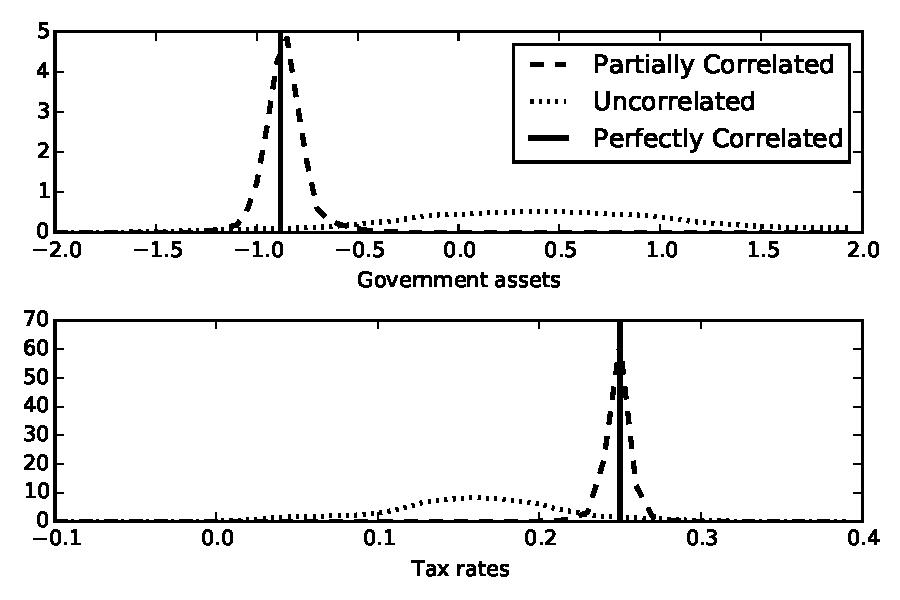
\includegraphics[width=7in]{plots/ErgodicQL.pdf}
 \caption{Ergodic distribution for debt and taxes in the representative agent quasilinear economy for three choices $P(s)$.}
 \label{fig: ergodic distribution ql}
 \end{figure}



\subsection{Heterogeneous agents}
\label{Sec: het agent}
In this section we turn to general problem of characterizing outcomes in an economy with heterogeneous agents and  transfers. In particular we introduce a second agent who has zero productivity and impose a non negativity constraint on his consumption. Given the Ricardian equivalnce result discussed in section \ref{Sec: ricardian eq}, we maintain a normalization that assets of the unproductive agent are zero throughout this section.
\begin{assumption}
The productivity of agents are ordered, $\theta_1>\theta_2=0$  and $c_{2,t}\geq 0.$
\end{assumption}
Before we discuss the results, a few words on the assumptions are pertinent. The assumption that $\theta_2=0$ makes the problem tractable and allows us to obtain a complete characterization of the problem as we wary the Pareto weights. The restriction on consumption is necessary to add  curvature to the problem. In more general settings risk aversion will impose Inada restrictions that play a similar role. We now state the theorem and then discuss its implications.



\begin{theorem}
Let $\omega,n$ be the Pareto weight and mass of the productive agent with $n<\frac{\gamma}{1+\gamma}$. The optimal tax, transfer and asset policies $\{\tau_t,T_t,B_t\}$ are characterized as follows,


\begin{enumerate}
 \item For $\omega\geq n \left(\frac{1+\gamma}{\gamma}\right)$ we have  $T_t=0$ and the optimal policy is same as in a representative agent economy studied in Theorems \ref{thm: rep agent general theorem},and \ref{thm: rep agent linear policies}
 \item For $\omega< n \left(\frac{1+\gamma}{\gamma}\right)$, suppose we further assume that $\min_{s}\{P(s)\}>\beta$. We have two parts:
 
 There exists $\mathcal{B}(\omega)$ and $\tau^*(\omega)$ with $\mathcal{B}'(\omega)>0$ and $\lim_{\omega\to 0}\mathcal{B}(\omega)<0$ such that 
 \begin{enumerate}
  \item $B\_>\mathcal{B(\omega)}$
\[T_t>0, \quad \tau_t=\tau^*(\omega), \textit{ and } B_t=B\_ \quad \forall t\] 
\item $B\_\leq \mathcal{B(\omega)}$, the policies depend on the structure of $P(s)$. 
\begin{enumerate}
 \item For $P(s)\not \in \mathcal{P}^*$
 
   \[\lim_t T_t>0 \text{ i.o.},\quad \lim_t\tau_t=\tau^*(\omega) \text{ and } \lim_tB_t=\mathcal{B}(\omega)\quad \textit{a.s}\]

 \item For $P(s)\in \mathcal{P}^*$we have two cases depending on $B\_$
\begin{enumerate}
 \item For $B\_\leq B^*$ 
 \[T_t = 0, \quad \lim_t \tau_t=\tau^{**} (\omega), \textit{ and } \lim_tB_t=  B^*\quad a.s \]
\item For $\mathcal{B}(\omega)>B\_>B^*$
\small
\[\Pr\{\lim_t T_t = 0, \lim_t \tau_t=\tau^{**}(\omega),\lim_tB_t=  B^* \textit{ or } \lim_t T_t>0 \text{ i.o.},\lim_t\tau_t=\tau^*(\omega), \lim_tB_t=\mathcal{B}(\omega) \}>0 \]
 \normalsize 
\end{enumerate}


 \end{enumerate}

 \end{enumerate}

 \end{enumerate}


\end{theorem}

The main concern in this setting with heterogeneous agents  is that costs of fluctuating transfers to hedge aggregate shocks are endogenous. The simplifications in the environment allow us to highlight how these depend on the Pareto weights (relative to the mass ) of the Planner: $\{\omega,1-\omega\}$ corresponding to Agents 1 and 2 respectively. A regressive planner who cares a lot about the productive agents in effect faces high costs of using transfers. For such a planner (with a high $\omega$), increasing transfers also means giving resources to the unproductive agent whose consumption he does not value as much. In fact the threshold $\bar{\omega}=n\left(\frac{1+\gamma}{\gamma}\right)$ is such that above this, transfers are never used and thus the allocations are identical to the representative agent economy studied before. 

For a less regressive planner (such that $\omega<\bar{\omega})$ transfers are an important tool for redistributing resources to the unproductive agent in adverse times. To finance these these it taxes the productive agent and does not need to accumulates a large buffer stock of assets. Thus limiting assets are lower and tax rates are larger  for more redistributive planners.


\section{More general economies}
\label{Sec: more general economies}
The analysis in the previous section was simplified in many dimensions - no curvature on the utility from consumption, lack of persistence in shocks and restricting heterogeneity to two agents. The key implication we could thereby exploit was that the return on debt was exogenous, given by $\beta^{-1}P(s)$. Adding curvature makes these returns endogenous even for standard risk free bond with a payoff vector $P(s)=1$. Technically, it requires us to additionally keep track relative marginal utilities to characterize how taxes, debt, and transfers react to shocks. This makes it harder to separate spanning and redistribution concerns. 

In the next section we first show that with risk aversion, exact spanning can occur only if shocks are binary and IID. For instance with CES preferences, the limiting allocation has constant relative consumptions and taxes rates. We show that how similar to the quasilinear case, the co movement of interest rates and exogenous shocks govern the governments' incentives to accumulate assets. 



\subsection{Spanning with binary shocks}

Let $\Psi \left( s;\bm{x},\bm{\rho },s\_\right) $ be an optimal  law of motion for the state variables
for the $t\geq1$ recursive problem, i.e., $\Psi \left( s;\bm{x},%
\bm{\rho },s\_\right) =\left( x^{\prime }\left( s\right) ,\rho ^{\prime
}\left( s\right) \right) $  solves (\ref{eq:BM2}) given state $\left(
\bm{x},\bm{\rho },s\_\right) .$
\begin{definition}
 A steady state  $\left( \bm{x}^{SS},\bm{\rho} ^{SS}\right) $  satisfies $\left(\bm{ x}^{SS},\bm{\rho}
^{SS}\right) =\Psi \left( s;\bm{x}^{SS},\bm{\rho} ^{SS},s_{-}\right) $ for all $%
\,s,s\_.$
\end{definition}
Since in this steady state $\rho_i =U_{c}^{i}(s)/U_{c}^{1}(s)$ does
not depend on the realization of shock $s,$ the ratios of marginal utilities
of  all agents are constant. The continuation allocation depends only on  $s_{t}$ and not on the  history $s^{t-1}$.% These outcomes are reminiscent though not quite identical to those in a complete market economy (see Werning
%2007).\footnote{\textcolor{blue}{David, I have changed it a bit, do you think it reflects our understanding better. The earlier one sounded too cautionary}
%The steady state allocation is optimal for a \emph{modified} complete market problem where the Planner has to additionally adhere to a specific ratio of pairwise consumption (or ``market weights'' as in Werning(2007). However we note that typically, there does not exist an initial distribution of  assets  and list of Pareto weights for which the optimal allocation with complete markets will \emph{coincide} with the aforementioned stationary allocation with incomplete markets.}

We  begin by noting that a competitive equilibrium fixes an allocation $\{c_i(s),l_i(s)\}_{i}$ given a choice for $\{\tau(s), \bm{\rho}(s)\}$ using equations (\ref{eq:BM2_Wages_cons}), (\ref{eq:BM2_Res_cons}) and (\ref{eq:BM2_rhoprime}).  Let us denote $U(\tau,\bm{\rho},s)$ as the value for the planner from the implied allocation using Pareto weights $\{\omega_i\}_i$ ,
\[U(\tau,\bm{\rho},s)=\sum_{i}\omega_i U^i(s).\]

As before define $Z_i(\tau,\rho,s)$ as
\[Z_i(\tau,\bm \rho,s)=U^i_c(s)c_i(s)+U^i_l(s)l_i(s)-\rho_i(s)\left[U^1_c(s)c_1(s)+U^1_l(s)l_1(s)\right].\]

% Note that $\sum_{i=2}^{N}Z_i(\tau,\bm  \rho,s)$ is the marginal utility adjusted  primary deficit using the implied allocation.
%
%
%
% %Next we define $Z(\tau,\rho,s)$ as the marginal utility adjusted primary deficit using the implied allocation.
% \[Z(\tau, \bm \rho,s)=c_1^{-\sigma}(s)\left\{NT(s)+g-\tau(s)\sum_{i=1}^{N}\left[\theta_il_i(s)\right]\right\}\]
%
%
For the IID case,  the optimal policy  solves the following Bellman equation for $\bm{x}(s^{t-1})=\bm{x},\bm{\rho}(s^{t-1})=\bm{\rho}$
%
 \begin{equation}
 \label{eq:ss-obj}
 	V(\bm x,\bm \rho) = \max_{\tau(s),\bm \rho'(s),\bm x'(s)}\sum_s \pi(s)\left[ U(\tau(s),\bm \rho'(s),s) + \beta(s) V(\bm x'(s),\bm \rho'(s))\right]
 \end{equation}
subject to the constraints
 \begin{equation}
 \label{eq:ss-imp}
 	Z_i(\tau(s),\bm \rho'(s),s) + x'_i(s) = \frac{x_i \beta^{-1}P(s) U^i_c(\tau(s),\bm \rho'(s),s)}{\mathbb{E} U^i_c(\tau,\rho)}\text{   for all  $s,i \geq 2$,}\\
 \end{equation}
\begin{equation}
\label{eq:bondcondtion}
 	\sum_s \pi(s)P(s)U^1_c(\tau(s),\bm \rho'(s),s)(\rho_i'(s)-\rho_i) = 0 \text{  for $i \geq 2.$}
\end{equation}

 Constraint (\ref{eq:bondcondtion}) is obtained by rearranging constraint (\ref{eq:BM2_Bonds_cons}). It implies that $\rho(s)$ is a risk-adjusted martingale. We next check if the first-order necessary conditions are consistent with stationary policies for some ($\bm x, \bm \rho$).\footnote{Appendix \ref{apndx: numerical methods} discuses the associated second order conditions that ensure these policies are optimal}
 \begin{lemma}\label{lemma-simplified-foc}
With risk aversion $\|S\|=2$ is necessary for a steady state to exist
 \end{lemma}
 \begin{proof}
  
 
 
 
 Let $\pi(s)\mu_i(s)$ and $\lambda_i$ be the multipliers on constraints (\ref{eq:ss-imp}) and (\ref{eq:bondcondtion}).  Imposing the restrictions $x'_i(s) = x_i$ and $\rho'_i(s) = \rho_i$, at a  steady state  $\{\mu_i,\lambda_i,x_i,\rho_i\}^{N}_{i=2}$ and $\{\tau(s)\}_s$
are determined by  the following equations


\begin{subequations}
\label{sys-steadystate}
\begin{equation}
\label{eq:ss.imp.simplified}
  	Z_i(\tau(s),\bm \rho,s) + x_i = \frac{\beta^{-1}P(s)x_i U^i_c(\tau(s),\bm \rho,s)}{\mathbb{E} U^i_c(\tau,\rho)}\text{   for all  $s,i \geq 2$,}\\
\end{equation}
 \begin{equation}
	U_{\tau}(\tau(s),\bm \rho,s)-\sum_i\mu_i Z_{i,\tau}(\tau(s),\bm \rho,s)  =0 \text{  for all $s$,} \label{eq:foc.tau.simplified}\\
   \end{equation}
\begin{equation}
	U_{\rho_i}(\tau(s),\bm \rho,s) -\sum_j\mu_jZ_{j,\rho_i}(\tau(s),\bm \rho,s)+ \lambda_iP(s)U^1_c(\tau(s),\bm \rho,s)-\lambda_i\beta\mathbb{E}P(s)U^1_c(\tau(s),\bm \rho(s),s) =0. \text{   for all $s,i \geq 2$ }\label{eq:foc.R.simplified}
 \end{equation}

\end{subequations}



Since the shock $s$ can take only two values, \eqref{sys-steadystate} is a square system in $4(N-1)+2$ unknowns $\{\mu^{SS}_i,\lambda^{SS}_i,x^{SS}_i,\rho^{SS}_i\}^{N}_{i=2}$ and $\{\tau^{SS}(s)\}_{s}$. \end{proof}

The behavior of the economy in the steady state is similar to the behavior of the complete market economy characterized by Werning (2007). Both taxes and transfers depend only on the current realization of shock $s_t$. Moreover, the arguments of Werning (2007) can be adapted  to show that taxes are constant when preferences have a CES form $c^{1-\sigma}/(1-\sigma) - l^{1+\gamma}/(1-\gamma) $ and fluctuations in tax rates are very small when preferences take forms consistent with the existence of  balanced growth. We return to this point after we discuss convergence properties.

The previous calculations provides a simple way to verify existence of a steady state for wide range of parameter values by checking that there exists a root for system (\ref{sys-steadystate}). Since the system of equations (\ref{sys-steadystate}) is non-linear, existence can generally be verified only numerically. Next, we provide a simple example with risk averse agents in which we can show existence of the root of (\ref{sys-steadystate}) analytically. The analytical characterization of the steady state will help us  develop some comparative statics and build a connection from the quasilinear economy to the quantitative analysis to appear in section \ref{sec: numerical results}.

\subsubsection{A two-agent example}\label{sec: 2 agent example}


Consider an economy consisting of  two types of households with $%
\theta _{1,t}>\theta _{2,t}=0$. One period utilities are $\ln c-\frac{1}{2}%
l^{2}.$ The shock $s$  takes  two values, $s\in \left\{
s_{L},s_{H}\right\} $ with probabilities $\Pr \left( s|s\_\right) $ that are
independent of $s_{-}.$ We assume that $g\left( s\right) =g$ for all $s,$
and $\theta _{1}\left( s_{H}\right) >\theta _{1}\left( s_{L}\right) .$ We allow the discount factor $\beta(s)$ to depend on  $s.$

\smallskip

\begin{theorem}
\label{thm long run forces}\smallskip Suppose that $g<\theta (s)$ for all $%
s.$ Let $R(s)$ be the gross interest rates and $x=U^2_c(s)\left[b_2(s)-b_1(s)\right]$

\begin{enumerate}
\item \textbf{Countercyclical interest rates.} If $P \left( s_{H}\right) =P\left( s_{L}\right)$, then
there exists a steady state $\left( x^{SS},\rho ^{SS}\right) $ such that $%
x^{SS}>0,\ R^{SS}\left( s_{H}\right) <R^{SS}\left( s_{L}\right) .$
\item \textbf{Acyclical interest rates.}  There exists a pair $\left\{ P\left( s_{H}\right) ,P \left( s_{L}\right)
\right\} $ such that there exists a steady state with $x^{SS}>0$ and $R^{SS}\left(
s_{H}\right) =R^{SS}\left( s_{L}\right)$.
\item \textbf{Procyclical interest rates.} There exists a pair  $\left\{ P \left( s_{H}\right) ,P\left( s_{L}\right)
\right\} $ such that there exists a steady state with $x^{SS}<0$ and  $R^{SS}\left( s_{H}\right) >R^{SS}\left( s_{L}\right) .$
\end{enumerate}
In all cases, taxes $\tau(s)=\tau^{SS}$ are independent of the realized state.
\end{theorem}


In this two-agent case, by normalizing assets of the unproductive agent (using theorem \ref{theorem: main}) we can interpret $x$ as the marginal utility adjusted assets of the government. Besides establishing existence, the proposition identifies the importance of cyclical properties of real interest rates in determining the sign of these assets.

Proposition \ref{thm long run forces}  shows  two main forces that determine the dynamics of taxes
and assets: fluctuations in inequality and fluctuations in the interest rates. Let's start with part 2 of proposition \ref{thm long run forces}, which turns off the second force. When  interest rates are fixed, the government can adjust two
instruments in response  to an adverse  shock (i.e., a fall in $\theta_1$): it can either increase the  tax rate $%
\tau $ or it can decrease transfers $T.$ Both  responses are distorting,
but for different reasons. Increasing the tax rate increases distortions because the deadweight loss is convex in the tax rate,
 as in \cite{Barro1979}. This force operates in our economy just as it does in  representative agent economies.
 But in a  heterogeneous agent economy like ours,  adjusting transfers $T$ is
also costly. When agents' asset holdings are identical, a decrease in transfers  disproportionately
affects a low-skilled agent, so his marginal utility
falls by more than does the marginal utility of a high-skilled agent. Consequently, a
decrease in transfers increases inequality, giving rise to a cost  not present in  representative agent economies.

The government can reduce the costs of  inequality distortions by choosing
tax rate policies that make the net asset positions of  the high-skilled agent
decrease over time. That makes the two agents'
after-tax and after-interest income  become closer, allowing decreases in transfers to have smaller effects on inequality in
marginal utilities. If the net asset position of a high-skilled agent is
sufficiently low, then a change in transfers has no effect on inequality and
all  distortions from fluctuations in transfers are eliminated.\footnote{This convergence outcome has
 a similar flavor to "back-loading"\ results  of
 \cite{Ray2002} and \cite{Albanesi2012} that reflect the  optimality of structuring policies intertemporally eventually to disarm  distortions.}




%
% If consumption is ordered i.e it is higher in booms than in recessions, interest rates are countercyclical. The government will hold positive assets as long as the steady state marginal utility adjusted primary deficit$Z(\tau,\rho,s)$ is countercyclical too.

% It is possible to show numerically\footnote{Appendix \ref{apndx: numerical methods} describes a numerical test for existence and local stability cast in terms of  primitives.} that the steady state described in part
% 2 of  proposition \ref{thm long run forces} is stable, so the  economy converges to it. This convergence outcome has
% a similar flavor to "back-loading"\ results  of
% \cite{Ray2002} and \cite{Albanesi2012} that reflect the  optimality of structuring policies intertemporally eventually to disarm  distortions.

% Theorem \ref{theorem: main} provides  a useful way to compare our results with
%  representative agent economies. By that theorem, we can normalize $%
% b_{2,t}=0 $ for all $t$, in which case the negative of net assets of high-skilled agents can be
% interpreted as assets of the government. Because $x^{SS}>0,$
% the government  accumulates assets over time$,$ as in  AMSS.

% the government  accumulates assets over time$,$ as in  AMSS.

 Turning now to the second force,  interest rates generally fluctuate
 with  shocks.  Parts 1 and 3 of  proposition \ref{prop: long run forces} indicate what drives those  fluctuations. Consider again the example of a
 decrease in productivity of high-skilled agent. If the  tax rate  $\tau $ is left unchanged,
 the government faces a shortfall of revenues. Since
 $g$ is constant, the
 government requires  extra sources of revenues. But  suppose that
 the interest rate increases whenever $\theta_1 $ decreases, as happens, for
 example, with a risk free bond. If the government holds positive assets, its earnings from those assets increase. So holding assets allows higher interest income  to offset some of the government's revenue losses from taxes on labor.  The situation reverses if interest rates fall at
 times of increased need for government revenues, as in
  part 3 of  proposition \ref{prop: long run forces}, and the steady state allocation features the government's owning debt. 
  
  One can see the parallel with the representative agent quasilinear economy studied in section \ref{Sec: quasilinear}. There, exploiting linearity allowed us to provide a sharper characterization of how co-variance of interest rates with exogenous shocks affected the sign (and level) of debt through expression \ref{ss-debt}. In parts 1 and 3 of the propositon, with binary shocks,  altering the gap $P(s_H)-P(s_L)$ allows us to obtain the corresponding variation in interest rates. The resoning and the underling forces are exactly the same.
  
\subsection{Stability}
In this section we extend the approximation methods used to characterize outcomes in Theorem \ref{thm: rep agent linear policies} to the general problem with risk aversion. Unlike of obtaining an the quasilinear case where we could obtain analytical characterization, we present a test for convergence show local stability of a steady state for a wide range of parameters. 

As before, let assume that $\pi(s)\mu_i(s)$ and $\lambda_i$ be the multipliers on constraints (\ref{eq:ss-imp}) and (\ref{eq:bondcondtion}). In Appendix \ref{apndx: numerical methods} we show that the history-dependent optimal policies (they are sequences of functions of $s^t$) can be represented  recursively in terms of $\{\bm \mu(s^{t-1}),\bm \rho(s^{t-1})\}$ and $s_t$. A recursive representation of an optimal policy can be linearized around the steady state using $(\bm{\mu},\bm{\rho})$ as state variables.\footnote{One could  in principle look for a solution in state variables $\left(\bm{x}(s^{t-1}),\bm{\rho}(s^{t-1})\right)$. For $I=2$ with $\{\theta_i(s)\}$ different across agents, this would give identical policies and a map which is (locally) invertible between $\bm{x}$ and $\bm{\mu}$ for a given $\bm{\rho}$. However in other cases, it turns out there are unique linear policies in $(\
bm{\mu},\bm{\rho}
)$ and not necessarily in  $(\bm{x},\bm{\rho})$. This comes from the fact that the set of feasible $(\bm{x},\bm{\rho})$ are restricted at time 0 and may not contain an open set around the steady state values. When we linearize using $(\bm{\mu},\bm{\rho})$ as state variables, the optimal policies for $\bm{x}(s^t),\bm{\rho}(s^t)$ converge to their  steady state levels for all perturbations in $(\bm{\mu},\bm{\rho})$.}

Formally, let $\hat{\Psi}_{t}= \left[\bmat \bm{\mu}_{t} - \bm{\mu}^{SS}\\ \bm \rho_t - \bm \rho^{SS}\emat\right]$ be  deviations from a steady state. From a  linear approximation, one can obtain $B(s)$ such that
\begin{equation}
 \hat{\Psi}_{t+1}=B(s_{t+1})\hat{\Psi}_t. \label{eq.linear.lom}
\end{equation}
This linearized system has coefficients that are functions of the shock. The next proposition describes a simple numerical test that allows us to determine whether  this linear system converges to zero in probability.

\begin{theorem}\label{thm: localstability}
If the (real part) of eigenvalues of $\mathbb{E}B(s)$ are less than 1,  system (\ref{eq.linear.lom}) converges to zero  in mean. Further for large $t$, the conditional variance of $\hat{\Psi}$, denoted by $\Sigma_{\Psi,t}$, follows a deterministic process governed by
\[\text{vec}(\Sigma_{\Psi,t})=\hat{B} \text{vec}(\Sigma_{\Psi,t-1}),\]	
where $\hat{B}$ is a square matrix of dimension $(2I-2)^2$. In addition,  if the (real part) of eigenvalues of $\hat{B}$ are less than 1, the system converges in probability.
\end{theorem}

The eigenvalues (in particular the largest or the dominant one) are instructive not only for whether the system is locally stable but also how quickly the steady state is reached. In particular, the half-life of convergence to the steady state is given by $\frac{\log(0.5)}{\|\iota\|}$, where $\|\iota\|$ is the absolute value of the dominant eigenvalue.  Thus, the closer the dominant eigenvalue is to one, the slower is the speed of convergence.

We used Theorem \ref{thm: localstability} to verify local stability of a wide range of examples. Since the parameters space is high dimensional we relegate the comparative statics to Appendix \ref{}. The typical finding is that the steady state is stable and that convergence is slow. The rates of convergence are increasing in the covariance of interest rates and governments needs for revenue. 












\section{Numerical example}
\label{sec: numerical results}
In section \ref{} we used steady states to characterize the long-run behavior of optimal allocations and forces that guide the asymptotic level of net assets. 
In this section, we use a calibrated version of the economy to a) revisit the magnitude of these forces and and b) study optimal policy responses at business cycle frequencies when the economy is possibly far away from the steady state. We choose shocks and initial conditions to match stylized facts about recent
recession in US. The numerical calculations use methods adapted from Evans (2014) and described more in the Appendix \ref{}. The next section outlines how we choose the  parameters and initial conditions.
 


\subsection{Calibration}

We start with five types of agents\footnote{We report the results for $N=5$ to capture sufficient heterogeneity in wealth and earnings. Our methods allow us to solve for arbitrary number of agents and the qualitative/quantitative insights are unchanged by adding more intermediate types.} of equal measures with preferences $u(c,l)=\frac{c^{1-\sigma}}{1-\sigma}-\frac{l^{1+\gamma}}{1+\gamma}$. These agents will represent the $10\textsuperscript{th},25\textsuperscript{th},50\textsuperscript{th},75\textsuperscript{th},  \text{and } 90\textsuperscript{th}$ percentile of US wage distribution. 


We assume i.i.d aggregate shocks $\epsilon_t$ that affect labor productivities of each agent $\{\theta_{i,t}\}^{N}_{i=1}$ and payoff of the asset $p_t$ as follows,
\begin{subequations}
\begin{equation*}
\log \theta_{i,t}=\bar{\theta_i}\epsilon_t [1+(.9-i)m]
\end{equation*}
 \begin{equation*}
p_t=1+\chi \epsilon_t 
 \end{equation*}

\end{subequations}
Following \cite{Autor2008}, the average productivities $\{\bar{\theta_i}\}^{N}_{i=1}$ are set to match the respective earnings using Current Population Survey (CPS) that reports weekly earnings of full time wage and salary earners. 

The parameter $m$ allows us to generate recessions that lead to heterogeneous falls in income for different agents. We calibrate $m$ to match the facts reported \cite{Fatih2014}. Figure \ref{fig:fatih_picture} (adapted from their paper) reports that in the last recession the fall in income for the agents in the first decile of earnings was about  three times  that of the 90th percentile. Moreover between the 10th and the 90th change in the percentage drop in earnings was almost linear. This gives us a slope  $m=\frac{1.5}{0.8}$. 

 {
  \begin{figure}
  \label{fig:fatih_picture}
    \centering
    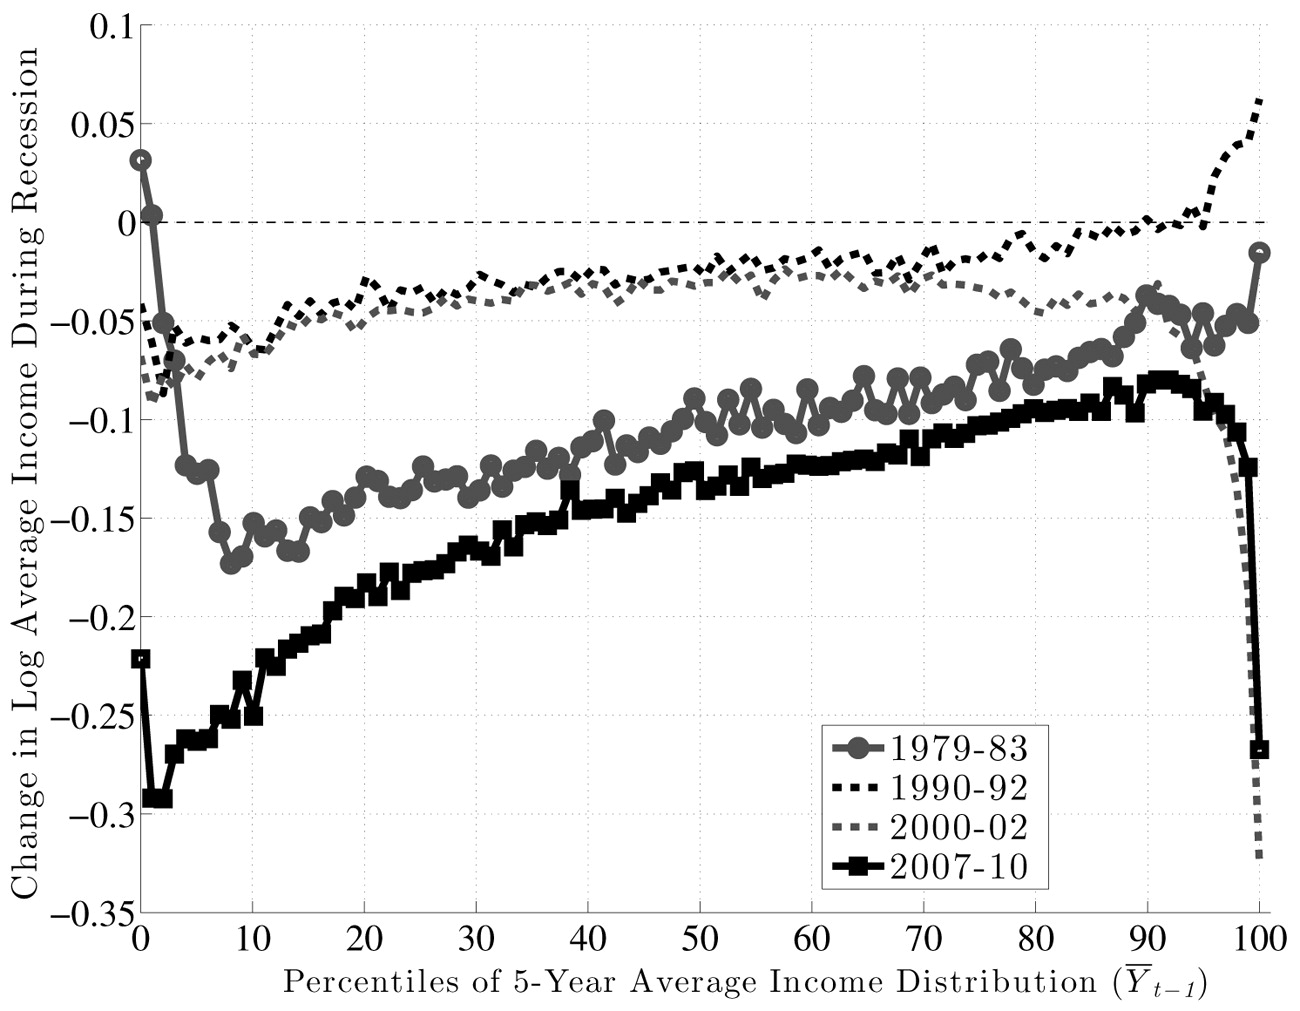
\includegraphics[width = 0.5\textwidth]{fg13.jpeg}
    \caption{ Change in log average earnings during recessions, prime-age males from \cite{Fatih2014}}
  \end{figure}

}

The parameter $\chi$ captures the ex-post co-movement in returns to government holdings and aggregate shocks. Our model takes no explicit stand where these come from. In principle they could capture variations in payoffs due inflation, interest rate risk (for longer maturity bonds) or defaults in some countries. For the purpose of the numerical exercise we use US data on inflation and interest rates of longer maturities bonds to calibrate $\chi$. This is described below:


Let $q^{(n)}_t$ be the log price of a nominal bond of maturity $n$. We can define the real holding period returns $r^{(n)}_{t,t+1}$ as follows
 
 \[r^{(n)}_{t,t+1}= q^{(n-1)}_{t+1}-q_t^{(n)}-\pi_{t+1}\]
 With the transfromation $y^{(n)}_t: -\frac{1}{n} q^{(n)}_t$ we can express $r^{(n)}_{t,t+1}$ as follows:
 \[r^{(n)}_{t,t+1}=\underbrace{y^{(n)}_t}_{\text{Ex-ante part}} - (n-1)\left[\underbrace{\left(y^{(n)}_{t+1}-y^{(n)}_{t}\right)}_{\text{Interest rate risk given $n$}}+\underbrace{\left(y^{(n-1)}_{t+1}-y^{(n)}_{t+1}\right)}_{\text{Term structure risk}}\right]-\underbrace{\pi_{t+1}}_{\text{Inflation risk}}\]

 In our model the holding period returns are given by $\log\left[\frac{p_{t+1}}{q_{t}}\right]$ and $q_t=\frac{\beta \mathbb{E}_tu_{c,t+1}P_{t+1}}{u_{c,t}}$. Note that $p_{t+1}$ allows us to captures ex-post fluctuations in returns to the government's debt  portfolio coming from maturity and inflation. 
 
The next table summarizes the co-movement between labor productivity $\{\epsilon_t\}$ and bond prices $\{q^{n}_t\}_{n}$ for different maturities (using quarterly data for the period XXXX to XXXX)
 
\begin{table}[htp]
\begin{tabular}{|l|l| l|l|l|}
\hline
Maturity (n) &2yr & 3yr & 4yr & 5yr\\
\hline
$Corr(\epsilon_{t+1},r^{(n)}_{t,t+1})$ & -0.11 &-0.093 &-0.083 &-0.072\\
$Corr(\epsilon_{t+1},r^{(n)}_{t,t+1}-ny^{(n)}_{t})$& 0.00 & -0.0463 &-0.080& -0.091\\
$Corr(\epsilon_{t+1},y^{(n)}_{t}-\pi_{t+1})$ &-0.097  &-0.086  &-0.080  &-0.073 \\ 
$\frac{\sigma({r^{n}_{t+1}})}{\sigma({\epsilon_{t+1}})}$  &0.820  &0.835  &0.843  &0.845\\ 
\hline 
\end{tabular}
\caption{}
\label{tab:corr}
\end{table}

The first line computes the correlation between the ex post returns and labor productivities.  In our baseline calibration, $\epsilon_{t}$ is i.i.d over time. Hence the parameter $\chi=\frac{\sigma_{r}}{\sigma_{\epsilon}} Corr(r,\epsilon)$. Averaging over different maturities gives us a value of $\chi=-0.06$. \footnote{The  second line of table \ref{tab:corr} computes only the correltaion of labor productivity with ex-post component of returns in the data. 
For the shortest maturity, 3 month real tbill returns $ Corr(\epsilon_{t+1},y^{1 qtr}_{t}-\pi_{t+1})=-0.11$. These results together give us range for $\chi$ of zero to negative $-0.09$. The numerical results are not sensitive to the value of $\chi$ is this range. } Thus payoffs are weakly countercyclical. Besides the results for the benchmark value of $\chi$, the long run simulations in the next section we will report the results a large range of $\chi$'s from $-1.0$ to $1.0$.

 
 
 We next turn to the parameters that describe the household preferences : We set risk aversion, $\sigma=1$, $\gamma=2$. This yields a Frisch elasticity of labor supply of $0.5$ and time discount factor, $\beta=0.98$ such that the annual interest rate in an economy without shocks is $2\%$ per year. 
 
 We assume that the initial wealth is perfectly correlated with wages and calibrate the wealth distribution to get the relative quantiles as in \cite{Kuhn2014} and Quadrini and Rios-Rull [2014]. These papers document the quantiles of net worth for US households computed up to 2010 Survey of Consumer Finances. 
 
 For the rest of parameters, namely Pareto weights and government expenditure, we use outcomes of the optimal allocation in the economy without shocks to target a (pre-trasnfers, federal) expenditure output ratio of $12\%$, tax rate of $23\%$, transfers to gdp of $10\%$ and debt to gdp of $100\%$. 
 


\begin{table}[htp]
\begin{tabular}{|l|c|p{4cm}|}
\hline
Parameter & Value & Description   \\ \hline
$\{\bar{\theta}_i\} $ & \{1 ,  1.4,  2.1,  3.24,  4.9\} & Wages dispersion for \{10,25,50,75,90\} percentiles   \\
$\gamma$ & 2 & Average Frisch elasticity of labor supply of 0.5 \\
$\beta$ & 0.98  &Average (annual) risk free interest rate of 2\%   \\
$m$ &$\frac{1.5}{.8}$& Heterogeneity in wage growth over business cycles\\
$\chi$ & -0.06 &Covariance between holding period returns and labor productivity\% \\
$\sigma_e$ & 0.03 & vol of labor productivity\\
$g$ & .13 \%&Average pre-transfer expenditure- output ratio of 12 \% \\\hline
\end{tabular}
\caption{Benchmark calibration}
\label{tab:Parameters}
\end{table} 
 
 
 
\subsection{Long run outcomes}
Figure \ref{fig:long_simulation} plots the simulated paths (of length 2000 periods) for debt to output ratio, labor tax rates and transfers to output ratio for three values of $\chi \in \{-1.0,-0.06,1.0\}$ in red, black and blue respectively. The three simulations have same initial conditions and sequence of underlying shocks. 


 {
  \begin{figure}
  \label{fig:long_simulation}
    \centering
    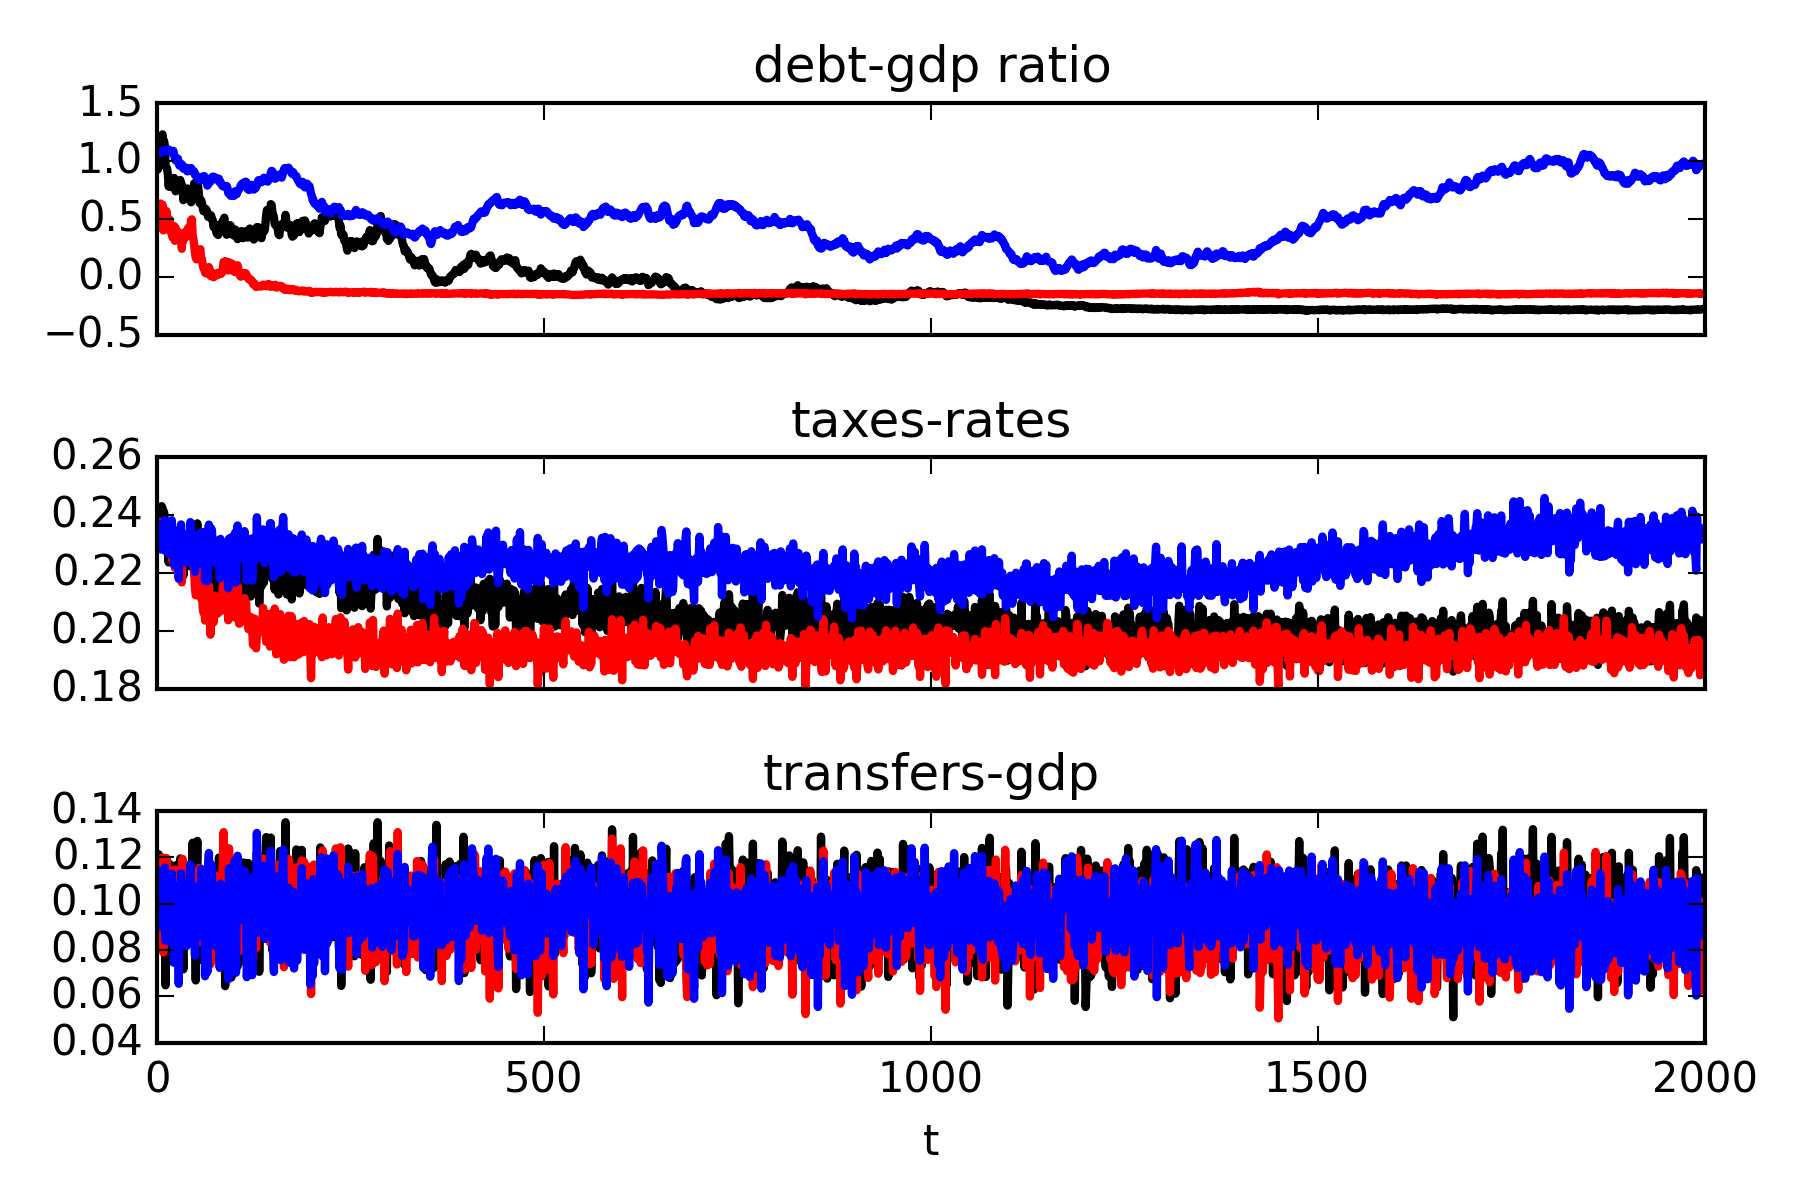
\includegraphics[width = 0.9\textwidth]{cesplots/long_simulation_debt.png}
    \caption{The red, black and blue lines plot simulations for a common sequence of shocks for values of $\chi=-1.5,0,1.5$ respectively}
  \end{figure}

}

Two features emerge: Different values $\chi$ have implications for position and speed of convergence for long run assets of the government. A sufficiently positive $\chi$ generates lower payoffs in recessions relative to booms. In line with theorem \ref{thm: rep agent general theorem} or theorem \ref{thm long run forces} , we see (blue line) that that  government does not repay its initial debt for 2000 periods. On the other had under the benchmark (black line) or the when $\chi$ is negative (red line), the government accumulates assets. 

In order to get a clearer picture of the speed of convergence, we plot the paths of the conditional means for debt and taxes in figure \ref{fig:speed_of_convergence}.  To explain how we generate these plots, let $B(s_{t+1},\bm x_t, \bm \rho_t)$ be the policy rules that generate the assets of the government and $\Psi \left( s_{t+1};\bm{x}_t,\bm{\rho }_t\right)$, the law of motion for the state variables. For a given history, the conditional mean of government assets is defined as follows:
\begin{subequations}
\begin{equation}
B^{cm}_{t+1}=\mathbb{E}B(s_{t+1},\bm x^{cm}_t,\bm \rho^{cm}_{t}) 
\end{equation}
 \begin{equation}
 \bm x^{cm}_t,\bm \rho^{cm}_{t}=\mathbb{E}\Psi (s_{t}, \bm x^{cm}_{t-1},\bm \rho^{cm}_{t-1}) 
 \end{equation}

\end{subequations}

Note that these paths smooths the high frequency movements in the dynamics of the state variables but retain the low frequency drifts. The different lines as before represent different values of $\chi$ between $-1.0$ and $1.0$ with the blue (red) lines representing positive (negative) values of $\chi$. The thickness of the lines represent larger values of $\chi$. The figure clearly shows the speed of convergence is increasing and the magnitude of the limiting assets in decreasing the strength of correlation between productivities and payoffs. This confirms the approximation results characterized in Theorem \ref{thm: rep agent linear policies}.

 {
  \begin{figure}
  \label{fig:speed_of_convergence}
    \centering
    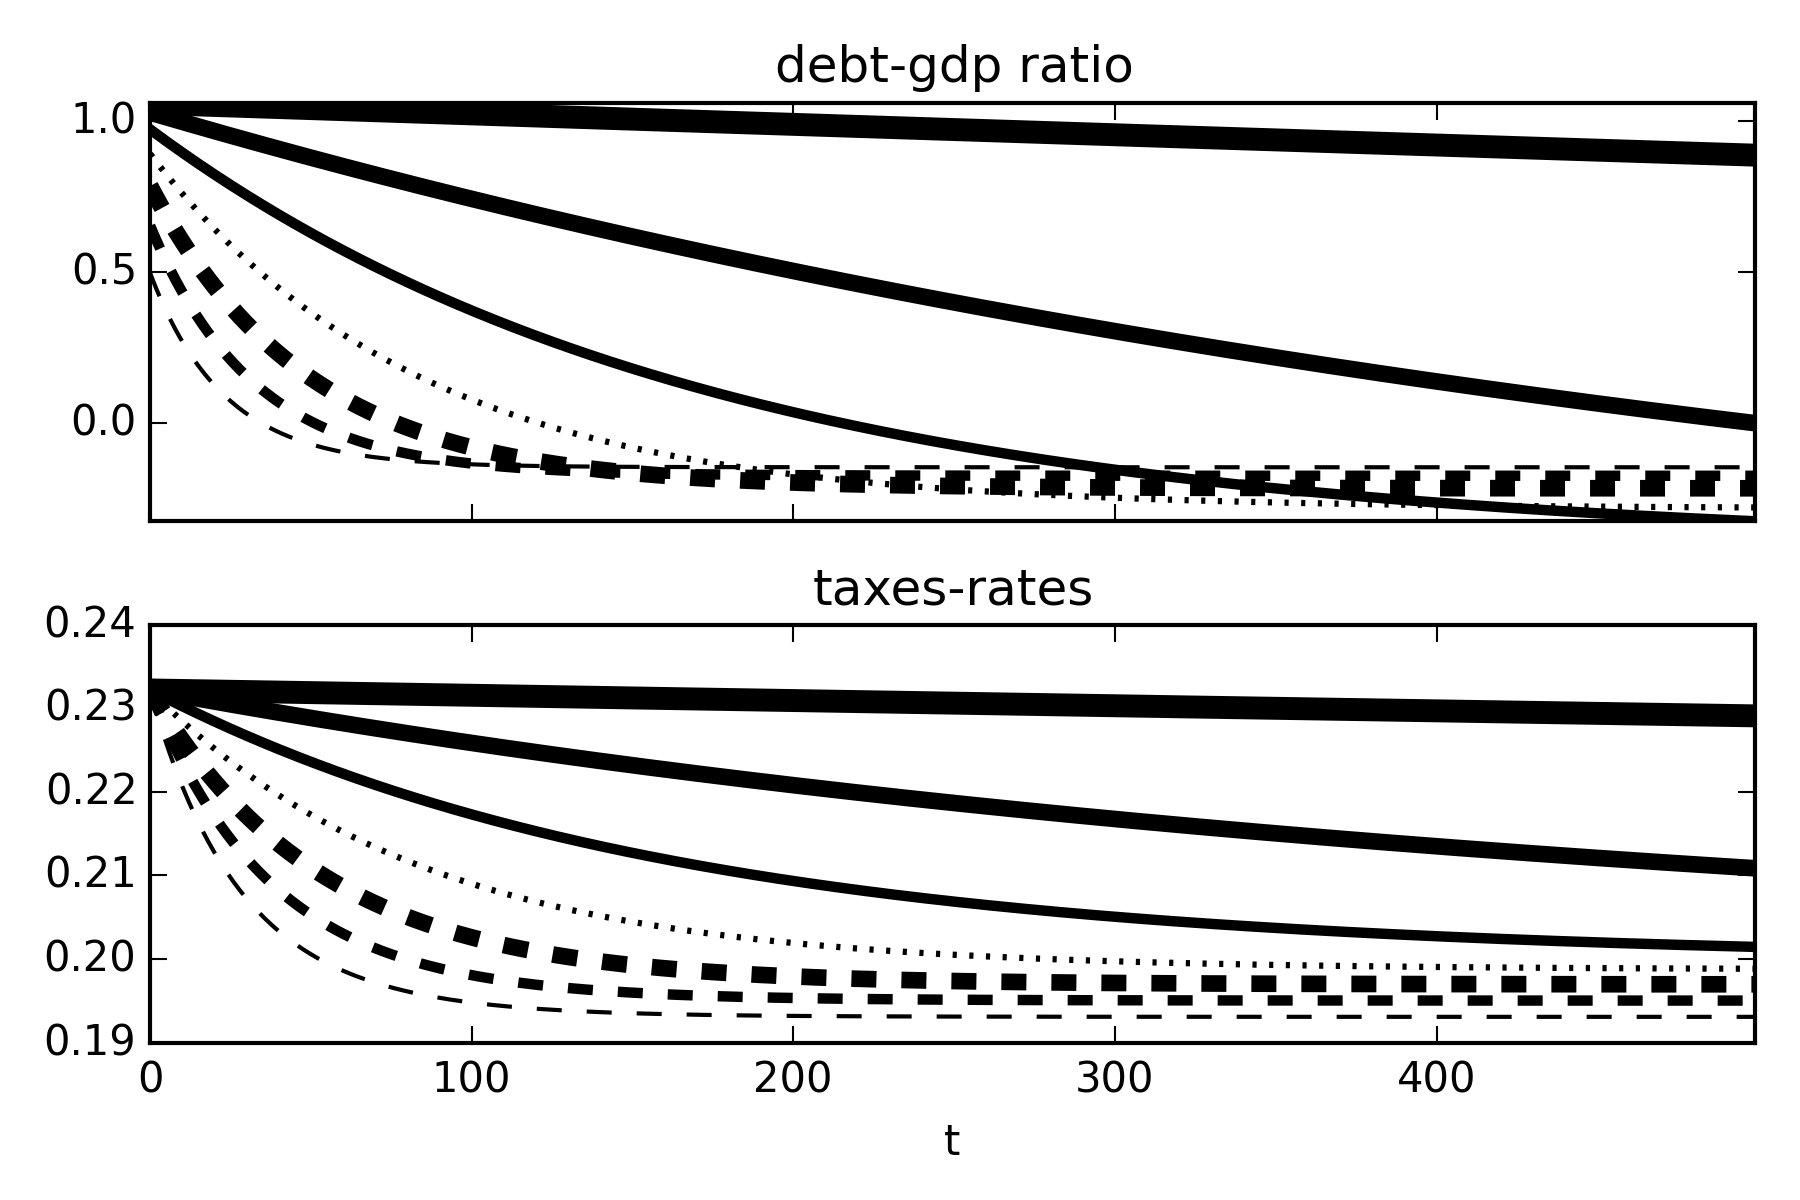
\includegraphics[width = .9\textwidth]{cesplots/speed_of_convergence.png}
    \caption{The plot shows conditional mean paths for different values of $\chi$. The red (blue) lines have $\chi<0$ ($\chi>0$). The thicker lines represent larger values.}
  \end{figure}

}


To verify the wide support of the ergodic distribution we take the initial conditions at the end of the long simulation and subject the economy to a sequence of 100 periods of $\epsilon_t$ shocks which are 2 standard deviations below the mean.  In figure \ref{fig: wide support of taxes} we see that given a sufficiently long sequence of negative productivity  shocks the economy will eventually deviate significantly from its ergodic mean.


{
  \begin{figure}
  \label{fig: wide support of taxes}
    \centering
    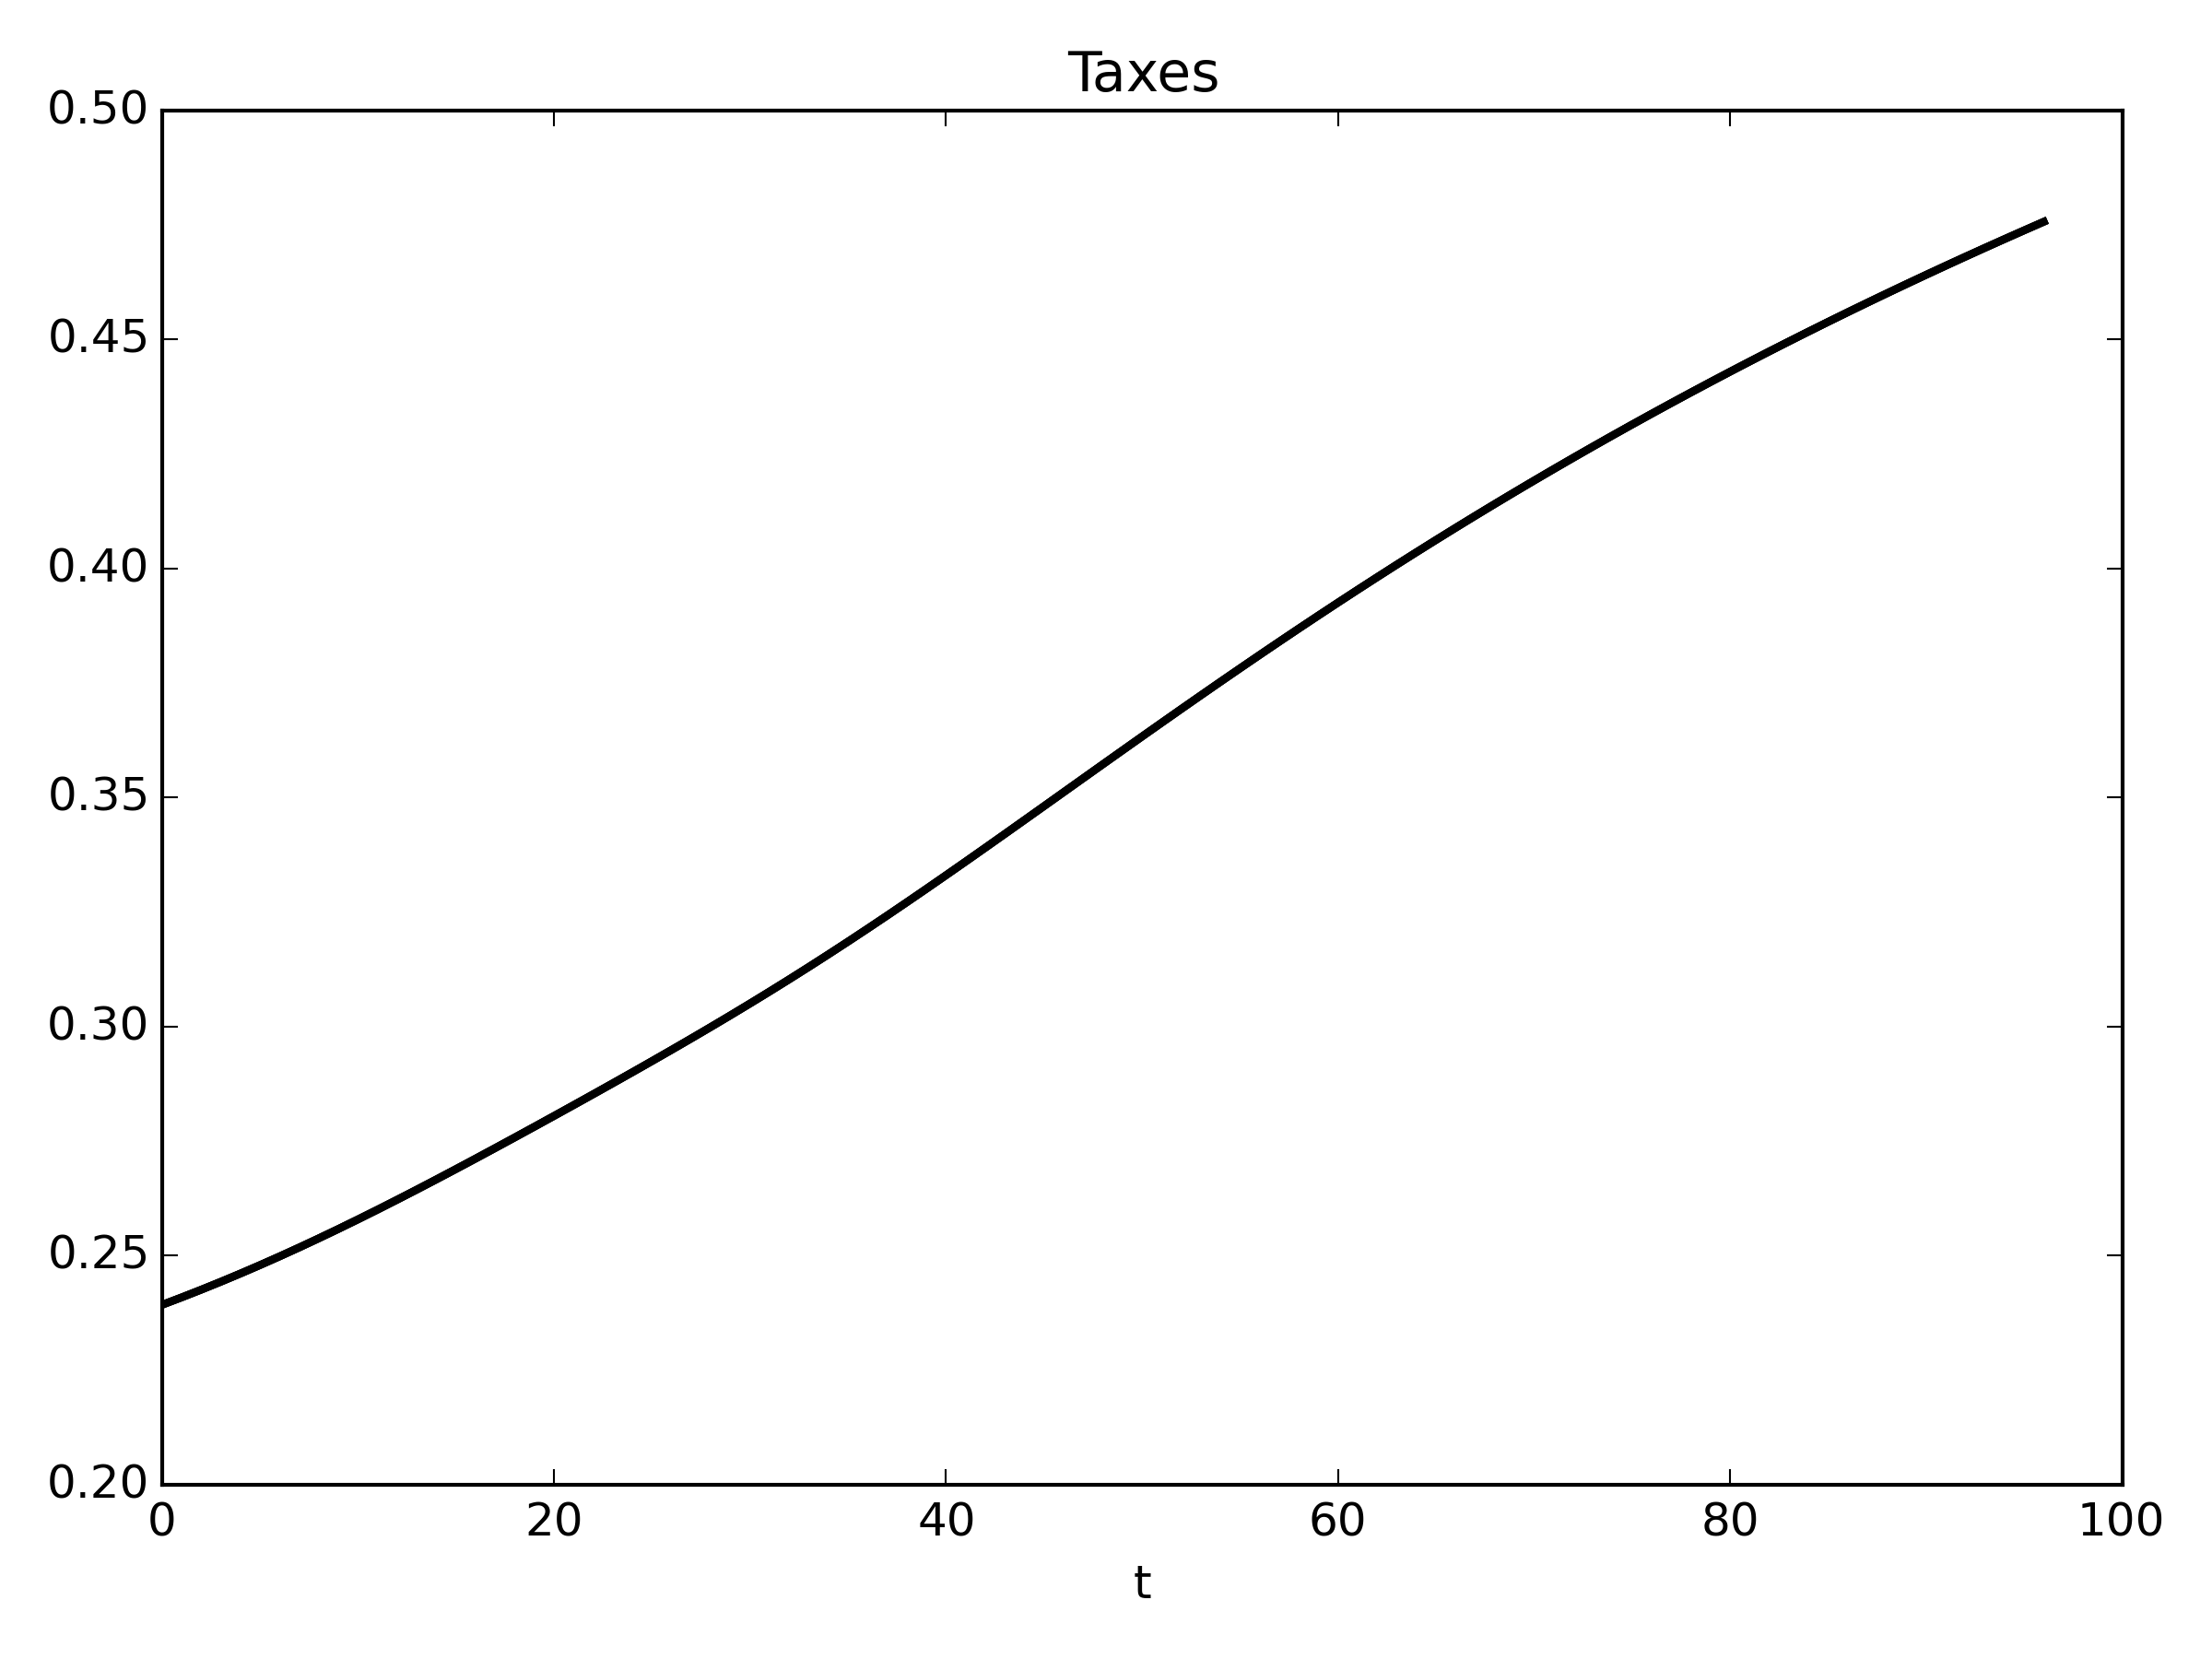
\includegraphics[width = 0.8\textwidth]{cesplots/taxes_only_bad_shocks.png}
    \caption{Taxes for a sequence of -1 s.d shocks to aggregate productivity of length 100}
  \end{figure}

} 

Our last conclusion was that the assets held by the government in the steady state was decreasing in the re-distributive motive of the government. We check this last part by changing the Pareto weights of the government.  In our baseline case the government places equal Pareto weights on all agents.  We introduce a re-distributive motive through a parameter $\alpha$.  The planner places evenly spaced Pareto weights from $0.2-\alpha$ on the lowest productivity agent to $0.2+\alpha$ on the highest productivity agent. 
Increases $\alpha$ decreases the concerns for redistribution.  We plot total assets of the government in steady state as a function of alpha in figure \ref{fig: comp_statics} and see that the relationship does indeed hold.


 
\subsection{Short run}
The analysis of the previous subsection studied  aspects of very low
frequency components of  the optimal policy. Here  we focus on business cycle frequencies.
 In our setting,  these higher frequency responses can conveniently be divided  into the magnitudes of changes as we switch from ``boom''
to ``recession,'' and the dynamics during  periods when a recession or boom state persists. A recession is a negative $-1.0$ standard deviation realization for the $\epsilon_t$ process. Given the initial conditions and the benchmark calibration, the plots below trace the paths for debt, taxes and transfers for sequence of shocks that feature a recession of four periods from $t=3$. Before and after this recession, the economy receives $\epsilon_t=0$.

The main exercise here is to compute how optimal taxes, transfers and debt in recessions accompanied by larger inequality are different in a recession that affects all agents alike. Under the benchmark calibration, log wages for agent $i$ are given by $\log \theta_i=\epsilon [1+(.9-i)m]$. We decompose the total responses into an only TFP  component by (by setting $m=0$) and an inequality component as follows:
  
\begin{equation*}
\log \theta^{tfp}_i=\epsilon 
\end{equation*}

\begin{equation*}
 \log \theta^{ineq}_i=\epsilon [(.9-i)m]
\end{equation*}

Figure \ref{fig: irf} plots the short run impulse responses. The shaded region is the induced recession and the bold line captures the the benchmark (total) response. The dashed (dotted) line
reflects the only TFP (inequality) effect. 
In the benchmark, the government responds to an adverse shock by a making big increases in transfers, the  tax rate, and  government debt. However, without inequality shocks (dotted line), the government
responds by decreasing transfers and  increasing both debt and
the tax rate, but by an amount an order of magnitude smaller than in the benchmark. 
{
  \begin{figure}
  \label{fig: irf}
    \centering
    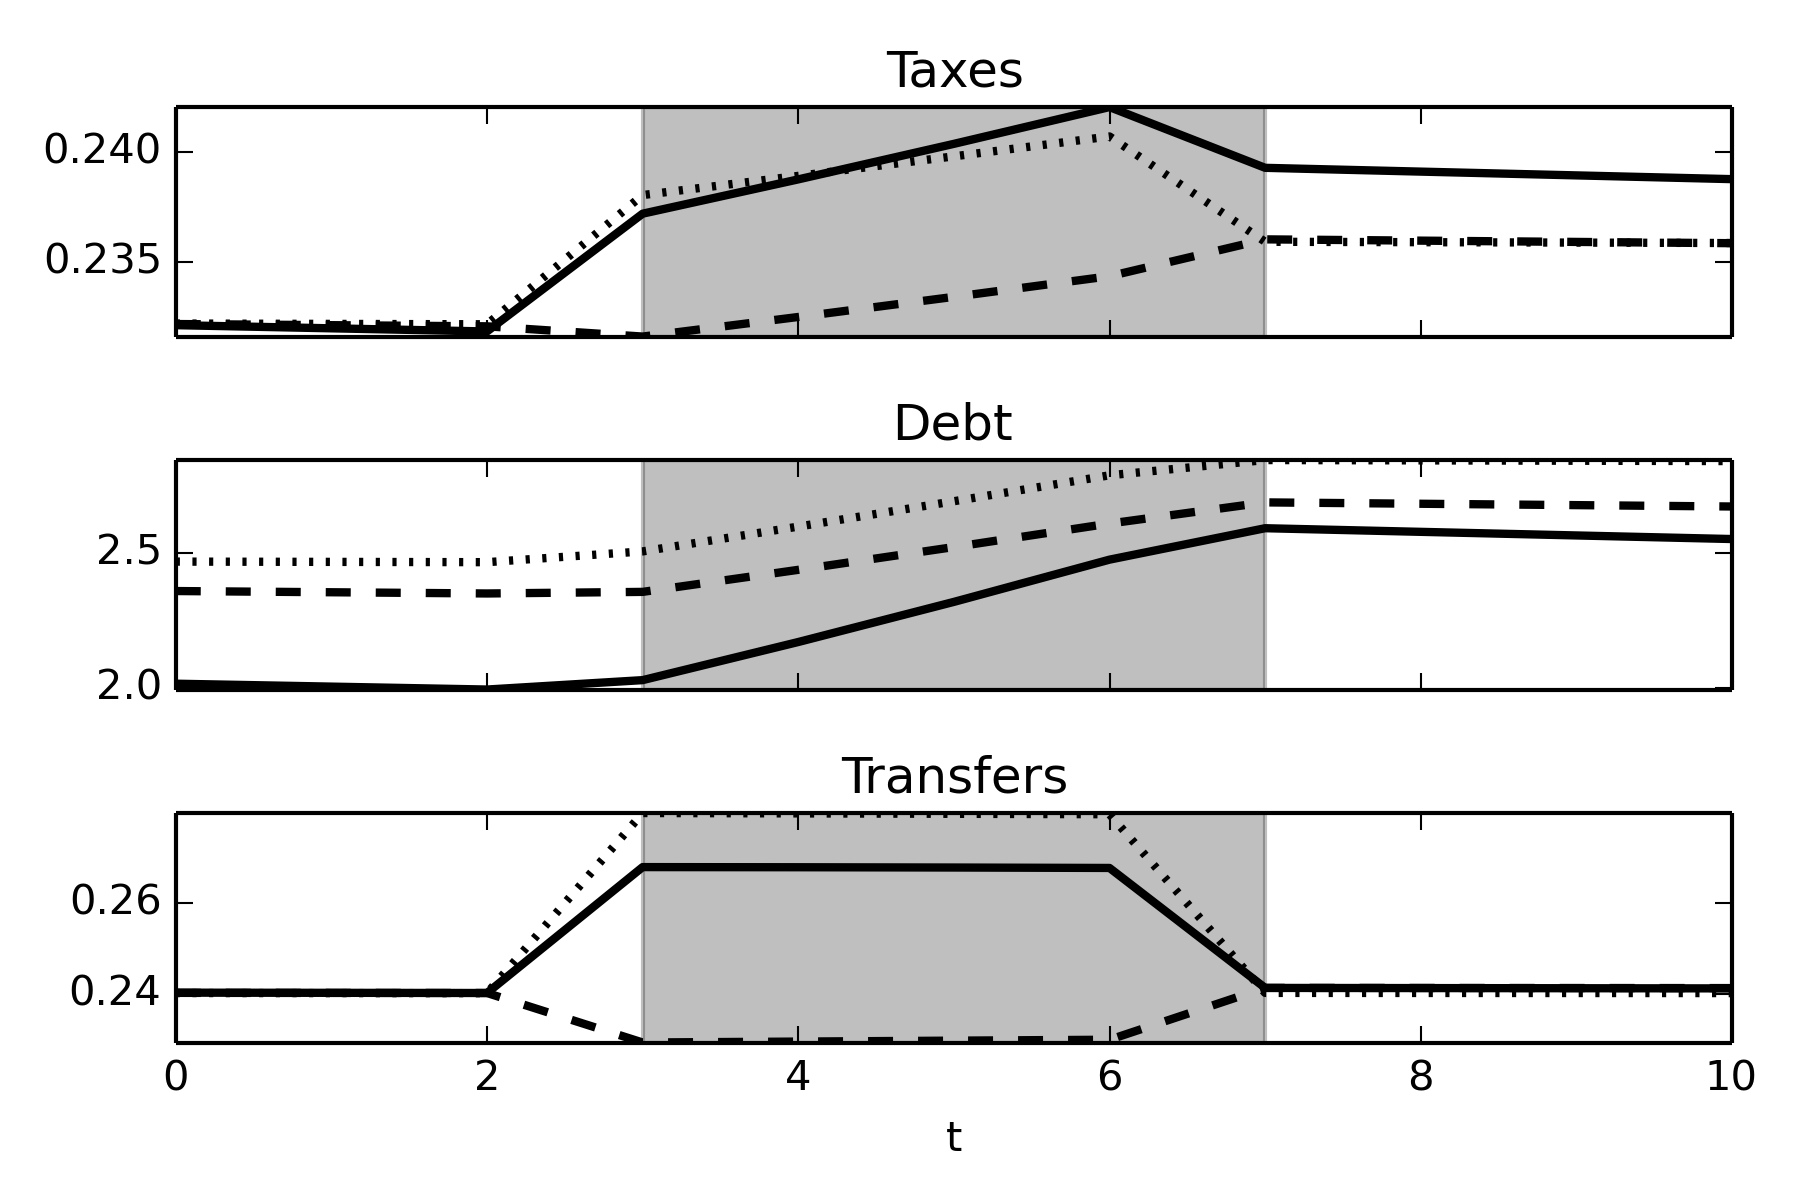
\includegraphics[width = 0.9\textwidth]{cesplots/irf_bm_chi_shocks.png}
    \caption{The bold line is the total response. The dashed (dotted) line reflects the only TFP (inequality) effect. The shaded region is the recession}
  \end{figure}

}
Next we average over sample paths of length 100 periods and report the volatility, autocorrelation and correlation with exogenous shocks for taxes and transfers in table \ref{tab:corr}. We see that taxes are twice as volatile and correlation between transfers and productivities switches sign. This  indicates that ignoring distributional goals can produce a misleading prescriptions for government
policy in recessions.

\begin{table}[htp]
\begin{tabular}{|l|l|l|}
\hline
Moments &Tfp& Tfp+Ineq\\\hline
vol. of taxes & 0.003&0.006\\
vol. of transfers &0.01 &0.02\\
autocorr. in taxes& 0.93&0.66\\
autocorr. in transfers& 0.17&0.18\\
corr. of taxes with tfp &0.15 &-0.63\\
corr. of transfers with tfp & 0.99&-0.98\\ \hline
\end{tabular}
\caption{Sample moments for taxes and transfers averaged across simulations of 100 periods}
\label{tab:corr}
\end{table}




\section{Conclusion}
\appendix
\section{Appendix}

\subsection{Extension: Borrowing constraints}\label{Sec: extensions}
%\textcolor{blue}{Anmol : I have removed proposition 2 and addeda mention that the corollary to theorem 1 is valid under adhoc borrowing constraints too. We dont have anything more to say about it. }
%
%\textcolor{blue}{Anmol : I have attempted to re-write the appendix in a way that it is self-contained. The earlier one had forward references and missing arguments.}

Representative agent models  rule out  Ricardian equivalence
either  by assuming distorting taxes or by imposing ad hoc borrowing constraints. %In section \ref{sec:Ricardian101},
By way of contrast, we have verified that Ricardian equivalence holds in our economy even though
there are distorting taxes. % are typically part of an optimal equilibrium.
Imposing ad-hoc borrowing limits also leaves Ricardian equivalence intact in our economy.\footnote{%
\citet{Bryant1984} describe how a government can use borrowing
constraints as part of a welfare-improving policy to finance exogenous
government expenditures. \citet{Sargent1987} describe Modigliani-Miller
theorems for government finance in a collection of economies in which
borrowing constraints on classes of agents produce the kind of rate of
return discrepancies that Bryant and Wallace manipulate.} In economies with
exogenous borrowing constraints, agents' maximization problems  include the
additional constraints
\begin{equation}
b_{i,t}\geq \underline{b}_{i}  \label{borrowing constraint}
\end{equation}%
for some exogenously given $\left\{ \underline{b}_{i}\right\} _{i}.$ %We
%define an equilibrium similarly to Definition \ref{Def: CE with affine taxes}%
\begin{definition}
\label{Def: CE with affine taxes borrowing constraints}For given $\left(
\left \{ b_{i,-1},\underline{b}_{i}\right \} _{i},B_{-1}\right) $ and $%
\left
\{ \tau _{t},T_{t}\right \} _{t},$ a competitive equilibrium with
affine taxes and exogenous borrowing constraints is a sequence $\{ \left \{
c_{i,t},l_{i,t},b_{i,t}\right \} _{i},B_{t},R_{t}\}_{t} $ such that $%
\left
\{ c_{i,t},l_{i,t},b_{i,t}\right \} _{i,t}$ maximizes (\ref{utility
lifetime})\ subject to (\ref{agent bc affine}) and (\ref{borrowing
constraint}), $\{ b_{i,t} \}_{i,t}$ are bounded,
and constraints (\ref{feasibility goods}), (\ref{govmt bc affine})\ and (\ref%
{feasibility bonds})\ are satisfied.
\end{definition}

We can define an \emph{optimal} competitive equilibrium with exogenous borrowing
constraints by extending Definition \ref{Def: optimal CE affine}.

%The role of the initial distribution of assets  is
%unaffected by the introduction of the ad-hoc debt limits and  so is Corollary  \ref{corr: B does not matter}.
The introduction of the ad-hoc debt limits leaves unaltered the conclusions of  Corollary  \ref{corr: B does not matter} and
the role of the initial distribution of assets across agents.
 The next proposition asserts
that ad-hoc borrowing limits do not limit a government's ability to respond to
aggregate shocks.\footnote{%
See \citet{Yared2012,Yared2013}  who shows a closely related result.}
\smallskip

\begin{proposition}
\label{thm:borrowing_constraint}  Given an initial asset distribution $\left(
\left\{ b_{i,-1}\right\} _{i},B_{-1}\right)$, let $\left\{ c_{i,t},l_{i,t}\right\} _{i,t}$ and $\left\{ R_{t}\right\}_t $ be a competitive
equilibrium allocation and interest rate sequence in an economy without
exogenous borrowing constraints. Then for any exogenous
constraints $\left\{ \underline{b}_{i}\right\} _{i}$, there is a government
tax policy $\left\{ \tau _{t},T_{t}\right\} _{t}$ such that $\left\{
c_{i,t},l_{i,t}\right\} _{i,t}$ is a competitive equilibrium
allocation in an economy with exogenous borrowing constraints $\left(
\left\{ b_{i,-1},\underline{b}_{i}\right\} _{i},B_{-1}\right) $ and $\left\{
\tau _{t},T_{t}\right\} _{t}.$
\end{proposition}

\begin{proof}
Let $\left\{ c_{i,t},l_{i,t},b_{i,t}\right\} _{i,t}$
be a competitive equilibrium allocation without exogenous borrowing
constraints. Let $\Delta _{t}\equiv \max_{i}\left\{ \underline{b}%
_{i}-b_{i,t}\right\} .$ Define $\hat{b}_{i,t}\equiv b_{i,t}+\Delta _{t}$ \ for all $t\geq 0$ and $\hat{b}_{i,-1}=b_{-1}.$ By Theorem %
\ref{theorem: main}, $\left\{ c_{i,t},l_{i,t},\hat{b}%
_{i,t}\right\} _{i,t}$ is also a competitive equilibrium allocation without
exogenous borrowing constraints. Moreover, by construction $\hat{b}_{i,t}-%
\underline{b}_{i}=b_{i,t}+\Delta _{t}-\underline{b}_{i}\geq 0$.
Therefore, $\hat{b}_{i,t}$ satisfies (\ref{borrowing constraint}). Since
agents' budget sets are smaller in the economy with exogenous borrowing
constraints, and $\left\{ c_{i,t},l_{i,t},\hat{b}%
_{i,t}\right\} _{i,t}$ are feasible at interest rate process $\left\{
R_{t}\right\} _{t}$, then $\left\{ c_{i,t},l_{i,t},%
\hat{b}_{i,t}\right\} _{i,t}$ is also an optimal choice for agents in the
economy with exogenous borrowing constraints $\left\{ \underline{b}%
_{i}\right\} _{i}.$ Since all market clearing conditions are satisfied, $%
\left\{ c_{i,t},l_{i,t},\hat{b}_{i,t}\right\} _{i,t}$ is a
competitive equilibrium allocation and asset profile.
\end{proof}

To provide some intuition for Proposition \ref{thm:borrowing_constraint}, suppose to the contrary that the exogenous borrowing constraints  restricted a  government's
 ability to achieve a desired allocation. That  means that
the government would want to increase  its borrowing
and to repay agents later, which the borrowing constraints prevent. But the government can just reduce
transfers today and increase them tomorrow. That would  achieve the  desired  allocation
without violating the exogenous borrowing constraints.

Welfare can  be strictly higher in an economy  with exogenous
borrowing constraints  relative to an economy without borrowing constraints because  a government might want to
push some agents against their borrowing limits. When agents' borrowing
constraints bind, their shadow interest rates differ from the
common interest rate that unconstrained agents face. When the government rearranges tax
policies to  affect the  interest rate, it affects constrained and unconstrained agents
 differently.  By facilitating
redistribution, this can improve welfare. %In the next several paragraphs, we will formalize this
%intuition.
We next construct an example without any
shocks in which the government can achieve higher welfare by using borrowing
constraints to improve its ability to redistribute.
In this section we construct an example in which the government can achieve
higher welfare in the economy with ad-hoc borrowing limits. We restrict ourselves to a deterministic economy with $g_t=0$, $\beta_t=\beta$ and $I=2$.  Further the utility function over consumption and labor supply $U(c,l)$ is separable in the arguments and satisfies the Inada conditions. The  planners problem can then be written as the following sequence problem
\begin{equation}
	\max_{\{c_{i,t},l_{i,t},b_{i,t},R_t\}_t} \sum_{t=0}^\infty\beta^t\left[\alpha_1U(c_{1,t},l_{1,t}) +\alpha_2 U(c_{2,t},l_{2,t})\right]\label{eq.A_obj}
\end{equation}subject to
\begin{subequations}
\begin{align}
	c_{2,t}+\frac{U_{l2,t}l_{2,t}}{U_{c2,t}}-\left(c_{1,t}+\frac{U_{l1,t}l_{1,t}}{U_{c1,t}}\right) +\frac{1}{R_t}\left( b_{2,t}-b_{1,t}\right)  = b_{2,t-1}-b_{1,t-1}\label{eq.A_imp}\\
	\frac{U_{l1,t}}{\theta_1U_{c1,t}} = \frac{U_{l2,t}}{\theta_2 U_{c2,t}}\label{eq.A_wage}\\
	c_{1,t}+c_{2,t} \leq \theta_1 l_{1,t}+\theta_2 l_{2,t}\label{eq.A_feas}\\
	\left(\frac{U_{ci,t}}{U_{ci,t+1}}-\beta R_t\right)(b_{i,t}-\underline b_i) = 0\label{eq.A_slack}\\
	\frac{U_{ci,t}}{U_{ci,t+1}} \geq \beta R_t\label{eq.A_euler}\\
	b_{i,t}\geq \underline b_i
\end{align}
\end{subequations}  Where $\underline b_i$ is the exogenous borrowing constraint for agent i.  We obtain equation \eqref{eq.A_imp} by eliminating transfers from the budget equations of the households and using the optimality for labor supply decision. Equations \eqref{eq.A_slack} and \eqref{eq.A_euler} capture the inter-temporal optimality conditions modified for possbily binding constraints.

Let $c^{fb}_i$ and $l^{fb}_i$ be the allocation that solves the first best problem, that is maximizing equation \eqref{eq.A_obj} subject to \eqref{eq.A_feas}, and define
\begin{equation}
	Z^{fb}  = c_{2}^{fb}+\frac{U_{l2}^{fb}l_{2}^{fb}}{U_{c2}^{fb}}-\left(c_{1}^{fb}+\frac{U_{l1}^{fb}l_{1}^{fb}}{U_{c1}^{fb}}\right)
\end{equation}and
\begin{equation}
	\tilde b_2^{fb} = \frac{Z^{fb}}{\frac1\beta -1}
\end{equation}  We will assume that the exogenous borrowing constraints satisfy $\underline b_2 = \underline b_1 + \tilde b_2^{fb}$.  We then have the following lemma

\begin{lemma}  If $\tilde b_2^{fb}>(<)0$ and $b_{2,-1}-b_{1,-1} > (<) \tilde b_2^{fb}$ then the planner can implement the first best.
\end{lemma}
\begin{proof}
We will consider the candidate allocation where $c_{i,t} = c^{fb}_i$, $l_{i,t} = l^{fb}_i$, $b_{i,t} = \underline b_i$ and interest rates are given by $R_t = \frac 1{\beta}$ for $t\geq 1$.  It should be clear then that equations \eqref{eq.A_wage} and \eqref{eq.A_feas} are satisfied as a property of the first best allocation.  Equation \eqref{eq.A_slack} is trivially satisfied since the agents are at their borrowing constraints.  For $t\geq 1$ equations \eqref{eq.A_imp} and \eqref{eq.A_euler} are both satisfied by the choice of $R_t = \frac1\beta$ and the first best allocations.  It remains to check that equation \eqref{eq.A_imp} is satisfied at time $t=0$ for an interest rate $R_0 <\frac1\beta$.  At time zero the constraint is give by
\begin{equation}
	Z^{fb} + \frac 1{R_0} \tilde b^{fb}_2 = b_{2,-1}-b_{1,-1}
\end{equation}  The assumption that $b_{2,-1}-b_{1,-1} > (<) \tilde b_2^{fb}$ if  $\tilde b_2^{fb}>(<)0$ then implies that
\[
	R_ 0 = \frac{\tilde b^{fb}_2}{b_{2,-1}-b_{1,-1}- Z^{fb}} <\frac 1\beta
\] as desired.
\end{proof}

This will improve upon the planners problem without exogenous borrowing constraints, as first best can only be achieved in this scenario when $b_{2,-1}-b_{1,-1} = \tilde b_2^{fb}$.

\bibliographystyle{econ_aer}
\bibliography{BEGS}
\newpage
\end{document}





\subsection{Representative agent}
\label{Sec: rep agent}
This section describes the representative agent environment with risky debt and no transfers. The household values consumption and leisure using a quasi-linear utility function and
solves
\begin{equation}
W_0(b_{-1})\max_{\{c_t,l_t,b_{t}\}_t}\mathbb{E}_0\beta^t\left \{c_t-\frac{l_t^{1+\gamma}}{1+\gamma}\right\}
\end{equation}
subject to
\begin{equation}
c_t+b_{t}=(1-\tau_t)\theta l_t+R_tP_tb_{t-t}
\end{equation}
Using the optimality condition for labor and savings we can summarize the set of implementability constraints for the government as follows
\begin{equation}
\label{rep agent QL seq implementability}
b_{t-1} \frac{P_t}{E_{t-1}P_t}=\mathbb{E}_t\sum_{j}\beta^{t+j}[c_{t+j}-l_{t+j}^{1+\gamma}] \quad \forall t
\end{equation}
We also have the feasibility constraint
\begin{equation}
\label{feasibility}
c_t+g_t\leq\theta l_t,
\end{equation}
and the market clearing for bonds $b_t+B_t=0$.





\noindent The optimal Ramsey allocation solves  $\max_{\{c_t,l_t\}_t}W_0(b_{-1})$ subject to \eqref{rep agent QL seq implementability}, feasibility \eqref{feasibility} and natural debt limits for the government $\underline{B}$\footnote{These will be explicitly derived for the examples we solve in this section.}. For the rest of the note we assume i.i.d exogenous shocks to expenditures denote expenditure and payoffs by $g_t=g(s_t)$and $P_t=P(s_t)$ with the normalization $\mathbb{E}P(s)=1$


\begin{theorem}
\label{rep agent general payoffs}

Suppose $P(s)$ satisfies \[P(s)-P(s')>\beta \frac{g(s)-g(s')}{\underline{B}} \quad \forall \quad s,s, \] there exists an invariant distribution of assets with unbounded support. Further for large enough assets (or debt) there is a drift towards the interior region. 

In particular $V$ is strictly concave and there exists $\underline{B}>B_1>B_2>-\infty$ such that

\[\mathbb{E}V'(B(s))>V'(B\_) \quad B\_>B_2 \]
and
\[\mathbb{E}V'(B(s))<V'(B\_) \quad B\_<B_1 \]

\end{theorem}


\begin{theorem}
\label{rep agent policy}
For the two special payoff structures, the optimal tax and asset policies $\{\tau_t,B_t\}_t$ are characterized as follows,
\begin{enumerate}
\item If $P(s)=1$ 
\[\lim_t \tau_t=-\infty, \quad \lim_t B_t=\infty    \quad a.s\]
\item If $P(s) = 1+ \frac{\beta}{ B^*}(g(s) - \mathbb{E} g)$ \quad for some $B^*\geq\underline{B}$
\[\lim_t \tau_t=\tau^*>\infty, \quad \lim_tB_t=  B^*\quad a.s \quad \forall B_{-1} \]

\end{enumerate}
 
\end{theorem}
%When the risky payoff on the bond $P(s)$ perfectly spans $g(s)$,
\begin{remark}
In the case where payoffs are perfectly correlated with expenditure shocks (case 2), we can express the long run assets \[B^*=\beta \frac{\var(g(s))}{\cov(P(s),g(s))}\]. Keeping tax rates (and hence tax revenues in this case) the government needs to finance a higher primary deficit when it gets positive expenditure shock. If in such states the assets pays off more, then optimally the government holds positive assets and uses the these high returns to finance this deficit. On the other hand if payoff are lower in times when the government needs resources, holding debt is valuable since it lowers the interest burden. Thus using the level of its assets $B^*$ it can perfectly span the fluctuations in deficits and the sign is given by the sign of the covariance of $P(s)$ with $g(s)$


The long run tax rate is inversely related to $B^*$ with the following limits,\[\lim_{B^*\to\underline{B}}\tau^*=\frac{\gamma}{1+\gamma}\quad \lim_{B^*\to\infty}\tau^*=-\infty\] 
 
\end{remark}


\begin{corollary}
Let $\underline{B}>-\infty$ be the natural debt limit for the government. Suppose we impose an upper bound on assets $\overline{B}<\infty$,

\begin{enumerate}
\item If $P(s) = 1+ \frac{\beta}{ B^*}(g(s) - \mathbb{E} g)$ \quad for some $\overline{B}>B^*\geq\underline{B}$
\[\exists \epsilon>0, \quad \Pr\{B_t<\underline{B}+\epsilon \text{ or } B_t>\overline{B}-\epsilon\}=0\]

\item For all other payoffs
\[\forall \epsilon>0, \quad \Pr\{B_t<\underline{B}+\epsilon \text{ and } B_t>\overline{B}-\epsilon \}=1\]
\end{enumerate}

\end{corollary}




  

\begin{theorem}
\label{rep agent ergodic distribution}
Consider a orthogonal decomposition of $P(s)$ as follows
\[P(s)=\hat{P}(s)+P^*(s)\] where
\[
  P^*(s) = 1+\frac{\beta}{B^*}( g - \mathbb{E} g) \text{ for some } B^*\geq \underline{B}
\]  
and $\hat{P}(s)$ is orthogonal to $g(s)$. Expanding the policy rules around the steady state of the $P^*(s)$ economy we have the following characterization,

\begin{itemize}
 \item The ergodic distribution of debt of the policy rules linearized around $(B^*, P^*(s))$ will have mean $B^*$, 
 \item The coefficient of variation is given by
  \[
    \frac{\sigma(B)}{\mathbb E(B)} = \sqrt\frac{\var(P(s)) - |\cov(g(s),P(s))|}{(1+|\cov(g(s),P(s))|)|\cov(g(s),P(s))|}\leq\sqrt\frac{\var(P(s)) - |\cov(g(s),P(s))|}{|\cov(g(s),P(s))|}
  \]
  \item The speed of convergence to the ergodic distribution described by
  \[
    \frac{\EE_{t-1}(B_t-B^*)}{(B_{t-1} - B^*)} = \frac1{1+|\cov(P(s),g(s))|}
  \]

\end{itemize}
  

\end{theorem}





\subsection{Heterogeneous agent: Quasi-linear unproductive agent}
Suppose the unproductive agent has quasi-linear preferences and we additionally impose a non negativity constraint on his consumption.
\begin{theorem}
Let $\omega,n$ be the Pareto weight and mass of the productive agent with $n<\frac{\gamma}{1+\gamma}$. The government trades a risky bond with payoffs $P(s)$ and faces i.i.d expenditure shocks.  The optimal tax, transfer and asset policies $\{\tau_t,T_t,B_t\}$ are characterized as follows,


\begin{enumerate}
 \item For $\omega\geq n \left(\frac{1+\gamma}{\gamma}\right)$ we have  $T_t=0$ and the optimal policy is same as in a representative agent economy studied in theorems \ref{rep agent general payoffs}, \ref{rep agent policy} and \ref{rep agent ergodic distribution}
 \item For $\omega< n \left(\frac{1+\gamma}{\gamma}\right)$, suppose we further assume that $\min_{s}\{P(s)\}>\beta$. We have two parts:
 
 There exists $\mathcal{B}(\omega)$ and $\tau^*(\omega)$ with $\mathcal{B}'(\omega)>0$ and $\lim_{\omega\to 0}\mathcal{B}(\omega)<0$ such that 
 \begin{enumerate}
  \item $B\_>\mathcal{B(\omega)}$
\[T_t>0, \quad \tau_t=\tau^*(\omega), \textit{ and } B_t=B\_ \quad \forall t\] 
\item $B\_\leq \mathcal{B(\omega)}$, the policies depend on the structure of $P(s)$. 
\begin{enumerate}
 \item For a risky bond with $P(s) = 1+ \frac{\beta}{ B^*}(g(s) - \mathbb{E} g)$ \quad for some $B^*<\mathcal{B}(\omega)$ we have two cases depending on $B\_$
\begin{enumerate}
 \item For $B\_\leq B^*$ 
 \[T_t = 0, \quad \lim_t \tau_t=\tau^{**} (\omega), \textit{ and } \lim_tB_t=  B^*\quad a.s \]
\item For $\mathcal{B}(\omega)>B\_>B^*$
\small
\[\Pr\{\lim_t T_t = 0, \lim_t \tau_t=\tau^{**}(\omega),\lim_tB_t=  B^* \textit{ or } \lim_t T_t>0 \text{ i.o.},\lim_t\tau_t=\tau^*(\omega), \lim_tB_t=\mathcal{B}(\omega) \}>0 \]
 \normalsize 
\end{enumerate}

\item For all other payoffs 
   \[\lim_t T_t=0 \text{ i.o.},\quad \lim_t\tau_t=\tau^*(\omega) \text{ and } \lim_tB_t=\mathcal{B}(\omega)\quad \textit{a.s}\]

 \end{enumerate}

 \end{enumerate}

 \end{enumerate}


\end{theorem}




% \begin{theorem}
% \label{main theorem}
% Suppose the Pareto weight of the agents are interior and we normalize the assets of the unproductive agent to zero. 
% Let $n$ and $\omega$ denote the mass and the Pareto weight of the productive agents. The optimal tax, transfer and debt policy $\{\tau_t,T_t,B_t\}_t$ is characterized as follows,
% \begin{enumerate}
% \item As $n\to 0$,
% \[\lim_t T_t=0,\quad \lim_t\tau_t=-\infty \text{ and } \lim_t B_t=\infty\]
% \item As $n\to 1$,
% \[\lim_t T_t=0 \text{ i.o.},\quad \lim_t\tau_t=\frac{-\gamma(\omega-n)}{\omega-(\omega-n)(1+\gamma)} \text{ and } \lim_tB_t=\mathcal{B}(\omega)<\infty\]
% \end{enumerate}
% 
% Furthermore $\mathcal{B}'(\omega)>0$ and $\lim_{\omega\to 0}\mathcal{B}(\omega)<0$
% \end{theorem}
% 
% \begin{corollary}
% Let $\underline{B}>-\infty$ be the natural debt limit for the government. Suppose we impose an upper bound on assets such that, $\mathcal{B}(\omega)<\overline{B}<\infty$. 
% \begin{enumerate}
% \item As $n\to 0$,
% \[\forall \epsilon>0, \quad \Pr\{B_t<\underline{B}+\epsilon \text{ and } B_t>\overline{B}-\epsilon \}=1\]
% \item As $n\to 1$,
% \[\exists \epsilon>0, \quad \Pr\{B_t<\underline{B}+\epsilon \text{ or } B_t>\underline{B}-\epsilon\}=0\]
% \end{enumerate}
% 
% 
% \end{corollary}


\section{Old Discussion}


The purpose of this note is to study the roles of transfers and debt as tools to hedge aggregate shocks in presence of  incomplete markets. 

We begin with the representative agent model studied in AMSS and make two changes:  first, the government trades a ``risky'' bond and second, the government  is prohibited 
from using transfers. The ``risky'' bond is a security whose payoffs $P_t(s^t)$ are correlated with the aggregate shocks. This feature allows us to vary the government's ability to span aggregate shocks while keeping markets incomplete. Below we will characterize two polar cases analytically: a) risk-free bond where $P_t(s^t)=1$ and b) perfect spanning where $\corr(P_t,g_t)=\pm 1$. Lastly we develop an approximation result for intermediate cases.

The main finding is that  the  levels and fluctuations in tax rates and government debt are both
driven by the covariance between  payoff on the bonds and the exogenous  needs for revenue  driven by exogenous government purchases.
With perfect spanning, the joint distribution of  long-run debt and taxes is degenerate, taxes and debt both  diverge in an economy with only
a risk-free bond being traded. The approximation result allows us to estimate the rates of convergence and volatility of debt and taxes for intermediate cases.

The restriction on transfers is meant to capture costs of using this instrument to hedge aggregate shocks. So far these costs are {\em ad hoc}
and assumed to be arbitrarily high. In the next section we endogenize these costs by adding concerns for redistribution and  allowing the government to choose transfers optimally. These concerns are be modeled by adding a positive
mass of unproductive but risk averse agents and assigning to  them a non-zero Pareto weight. Under the assumption that the government trades a risk free bond\footnote{The results for arbitrary payoffs extend analogously, i.e with perfect spanning the government eventually smooths fluctuations in both taxes and transfers.}
we construct two limiting cases of a representative agent economy by varying the mass of either type of agent.

The key insight is that the welfare costs of using fluctuating transfers to hedge aggregate shocks comes from 
the presence (and mass) of the unproductive risk averse agents. As their mass vanishes,
the optimal policy smooths labor taxes and all shocks are hedged by fluctuating transfers. 
In this case, asymptotically transfers diverge and tax rates approach zero. But when the mass of the productive agents is low, 
limiting transfers are constant. Eventually as their mass goes to zero, the optimal policy has unbounded labor subsidies and the level of transfers approaches zero.
In both cases the implied government assets (under the normalization that the unproductive agent holds no assets) diverge.

These limits can be contrasted with an alternative economy in which  the unproductive agents have quasi-linear preferences and 
we impose a non-negativity constraint on their consumption. As the mass of these unproductive agents approaches zero, 
limiting taxes are constant (they approach zero if their Pareto weight approaches zero too) but transfers are also zero infinitely often. The government accumulates a  finite level assets (typically positive). Thus the limiting allocation is similar to  that studied in AMSS with a non-negativity constraint on transfers where the government eventually accumulates first best level of assets. However, in our case these levels vary  inversely with the governments' preferences for redistribution and can switch signs for a low enough Pareto weight
on the productive agent. More regressive governments employ
tax subsidies and deficits that are financed by issuing debt. The optimal policy uses transfers as against accumulating assets to hedge aggregate shocks.

\section{Results left on the cutting board}

Besides the results mentioned before we have some things we proved that I could not fit. They mainly pertain to existence of steady state for more general preferences and shocks. I list them in this section


\subsection{Persistence}
\begin{theorem}
Consider a representative agent model studied in section \ref{Sec: rep agent} but with persistence shocks. For every complete market allocation indexed by $\mu^*$ there exists a payoff vector $P(s)$ such that there exists a  steady state in the risky debt economy that supports the same allocation. For an arbitrary payoff vector $P(s)$ (generically) there exists a steady state only if $\|S\|=2$
\end{theorem}


\subsection{Risk Aversion}
We have some scattered results for risk aversion and existence of steady state.
\begin{theorem}
Assume that $U$ is  separable and iso-elastic,	 $U(c,l) = \frac{c^{1-\sigma}}{1-\sigma} -\frac{ l^{1+\gamma}}{1+\gamma}$.
and shocks are i.i.d with $s_b$  being the ``adverse'' state (either low TFP or high govt. expenditures)
and $s_g$ begin the good state. Let $x_{fb}$ be the discounted present value of marginal utility weighted government surpluses associated with the first best allocation.
%\st{ be a value of  %\st{the state $x$ from which a government can implement first=best with complete markets}
%marginal utility weighted debt associated with the first-best allocation with complete markets.}\tjs{David: the phrase
%``first-best allocation with complete markets'' remains imprecise?  What does it mean?}
	 Let $q_{fb}(s)$ be the shadow price of government debt in state $s$ at the first best allocation.
	If
	\begin{equation}\label{eqn:prop52sufficient}
		\frac{1-q_{fb}(s_b)}{1-q_{fb}(s_g)} > \frac{g(s_b)}{g(s_g)}\geq 1 ,
	\end{equation}
		then there exists a steady state with $x_{fb}>x^*>0$
		\end{theorem}



\begin{theorem}
\label{thm long run forces}
Consider an economy consisting of  two types of households with $%
\theta _{1,t}>\theta _{2,t}=0$. One period utilities are $\ln c-\frac{1}{2}%
l^{2}.$ The shock $s$  is i.i.d and takes  two values, $s\in \left\{
s_{L},s_{H}\right\}.$ We assume that $g\left( s\right) =g$ for all $s,$
and $\theta _{1}\left( s_{H}\right) >\theta _{1}\left( s_{L}\right) .$ We allow the discount factor $\beta(s)$ to depend on  $s.$

\smallskip Suppose that $g<\theta (s)$ for all $%
s.$ Let $R(s)$ be the gross interest rates and $x=U^2_c(s)\left[b_2(s)-b_1(s)\right]$

\begin{enumerate}
\item \textbf{Countercyclical interest rates.} If $\beta \left( s_{H}\right) =\beta \left( s_{L}\right)$, then
there exists a steady state $\left( x^{SS},\rho ^{SS}\right) $ such that $%
x^{SS}>0,\ R^{SS}\left( s_{H}\right) <R^{SS}\left( s_{L}\right) .$
\item \textbf{Acyclical interest rates.}  There exists a pair $\left\{ \beta \left( s_{H}\right) ,\beta \left( s_{L}\right)
\right\} $ such that there exists a steady state with $x^{SS}>0$ and $R^{SS}\left(
s_{H}\right) =R^{SS}\left( s_{L}\right)$.
\item \textbf{Procyclical interest rates.} There exists a pair  $\left\{ \beta \left( s_{H}\right) ,\beta \left( s_{L}\right)
\right\} $ such that there exists a steady state with $x^{SS}<0$ and  $R^{SS}\left( s_{H}\right) >R^{SS}\left( s_{L}\right) .$
\end{enumerate}
In all cases, taxes $\tau(s)=\tau^{SS}$ are independent of the realized state.
\end{theorem}

\begin{remark}
 We can extend this result to the case with payoff shocks instead of discount factor shocks
\end{remark}
		
\begin{theorem}
\label{theorem}

Suppose the Pareto weight of the agents are interior and we normalize the assets of the unproductive agent to zero. 
Let $n \in [0,1]$ denote the mass of the productive agents. The optimal tax, transfer and debt policy $\{\tau_t,T_t,B_t\}_t$ is characterized as follows:
\begin{enumerate}
\item As $n\to 0$,
\[\lim_t T_t=0,\quad \lim_t\tau_t=-\infty.\]
\item As $n\to 1$,
\[\lim_t T_t=\infty,\quad \lim_t\tau_t=0.\]
\end{enumerate}
In both cases limiting government assets, $\lim_tB_t=\infty$ 


\end{theorem}
\begin{corollary}
Let $\underline{B}>-\infty$ be the natural debt limit for the government. Suppose we impose an upper bound on assets, $B_t\leq\overline{B}<\infty$
\[\forall \epsilon>0, \quad \Pr\{B_t<\underline{B}+\epsilon \text{ and } B_t>\overline{B}-\epsilon \}=1\]
\end{corollary}

		
		
\begin{theorem}
Consider an economy with at least two agents that are strictly risk averse and a shock process such that there exists a steady state. There do no exists initial conditions i.e a distribution of asset and a choice of Pareto weights such that this allocation can be supported as a complete market Ramsey allocation.
\end{theorem}
		
		

\newpage
\section{Appendix}
\appendix
{\textbf{Theorem 1}}
\begin{proof}




The optimal Ramsey plan solves the following Bellman equation. Let $V(b\_)$ be the maximum ex-ante value the government can achieve with debt $b\_$. 

\begin{equation}
  \label{eq-QLRA obj}
    V(b\_)=\max_{c(s),l(s),b(s)} \sum_{s}\pi(s)\left\{c(s)-\frac{l(s)^{1+\gamma}}{1+\gamma}+\beta V(b(s)) \right\}
\end{equation}   
subject to

   \begin{subequations}
   \label{sys- QLRA constraint}
    \begin{equation}
    \label{rep agent implementability constraint }
    c(s)+b(s)=l(s)^{1+\gamma}+\beta^{-1} P(s)b\_
    \end{equation}
 

 
\begin{equation}
  \label{eq-resoruces}
c(s)+g(s)\leq\theta l(s)
\end{equation}   
Let $\bar{b}=-\underline{B}$
\begin{equation}
  \label{ndl}
b\leq \bar{b}
\end{equation}   


   \end{subequations}
Let $\mu(s)\pi(s),\phi(s)\pi(s)$ be the Lagrange multipliers on the respective constraints. 


\begin{lemma}
There exists  a $\overline{b}$ such that $b_t\leq\overline{b}$. This is the natural debt limit for the government.
\end{lemma}
\begin{proof}
As we drive $\mu$ to $-\infty$, the tax rate approaches a maximum limit, $\bar{\tau}=\frac{\gamma}{1+\gamma}$. In state $s$, the government surplus,
\[
  S(s,\tau) = \theta^\frac\gamma{1+\gamma}(1-\tau)^\frac1\gamma\tau - g(s),
\]  which  is  maximized at $\tau = \frac\gamma{1+\gamma}$ when $(1-\tau)^\frac1\gamma\tau$ is also maximized. This would impose a natural borrowing limit for the government. 

\end{proof}

We begin with some useful lemmas

\smallskip To make this problem convex, let $L\equiv l^{1+\gamma }.$ 

Substitute for $c\left( s\right) $%
\[
V\left( b\_\right) =\max_{L(s),b(s)}\sum_{s\in S}\pi \left(
s\right) \left[ \frac{1}{1+\gamma }L\left( s\right) +\frac{1}{\beta }%
P\left( s\right) b\_-b\left( s\right) +\beta V\left( b\left( s\right)
\right) \right] 
\]%
s.t.%
\begin{eqnarray*}
\frac{1}{\beta }P\left( s\right) b-b\left( s\right) +g\left( s\right) &\leq
&\theta L^{\frac{1}{1+\gamma} }\left( s\right) -L\left( s\right) \\
b\left( s\right) &\leq &\bar{b} \\
L\left( s\right) &\geq &0.
\end{eqnarray*}

\begin{lemma}
\smallskip $V\left( b\right) $ is stictly concave, continuous,
differentiable and $V\left( b\right) <\beta ^{-1}$ for all $%
b<\bar{b}.$ The feasibility constraint binds for all $b\in (-\infty ,\bar{b}%
],\ s\in S$ and $\left( L^{\ast }\left( s\right) \right) ^{1-\frac{1}{1+\gamma} }\geq
\frac{1}{1+\gamma} .\footnote{
This last condition simply means that we do not tax to the right of the peak
of the Laffer curve. The revenue maximizing tax is $1-\bar{\tau}=\frac{1}{%
1+\gamma }.$ At the same time $1-\tau =l^{\gamma}$ so if taxes are always
to the left of the peak, $\frac{1}{1+\gamma }\leq l^{\gamma }=\left(
L^{\frac{1}{1+\gamma} }\right) ^{\gamma}=L^{1-\frac{1}{1+\gamma} }$.}$ 
\end{lemma}

\begin{proof}
\smallskip \textit{Concavity}

$V\left( b\right) $ is concave because we maximize linear objective
function over convex set.

\textit{Binding feasibility}

Suppose that feasibility does not bind for some $b,s.$ Then the optimal $%
L\left( s\right) $ solve $\max_{L\left( s\right) \geq 0}\pi \left( s\right) 
\frac{\gamma}{1+\gamma }L\left( s\right) $ which sets $L\left( s\right)
=\infty .$ This violates feasility for any finite $b,b\left( s\right) .$

\textit{Bounds on }$L$

Let $\phi\left( s\right) >0$ be a Lagrange multiplier on the
feasibility. \ The FOC for $L\left( s\right) $ is 
\[
\frac{1}{1+\gamma }+\phi(s) \left( \frac{1}{1+\gamma }L(s)^{\frac{1}{1+\gamma}
-}-\theta \right) =0. 
\]%
This gives%
\[
\frac{1}{1+\gamma }L^{\frac{1}{1+\gamma} -1}-\theta =-\frac{1}{\lambda }\frac{\gamma}{%
1+\gamma }<0 
\]%
or%
\[
L^{1-\frac{1}{1+\gamma} }\geq \frac{\theta }{1+\gamma }. 
\]

\textit{Continuity}

For any $L$ that satisfy $L^{1-\frac{}{1+\gamma} }\geq \frac{\theta }{1+\gamma} ,$ define function $%
\Psi $ that satisfies $\Psi \left( L^{\frac{1}{1+\gamma} }-\theta L\right) =L.$ Since $%
L^{\frac{1}{1+\gamma} }-L$ is strictly decreasing in $L$ for $L^{1-\frac{1}{1+\gamma} }\geq
\frac{1}{1+\gamma} $, this function is well defined. Note that $\Psi \left(
{}\right) \underbrace{\left( \frac{1}{1+\gamma }L^{\frac{1}{1+\gamma} -1}-\theta \right) }%
_{<0}=1$ (so that $\Psi >0$, i.e. $\Psi $ is strictly decreasing)
and $\Psi ^{\prime \prime }\underbrace{\left( \frac{1}{1+\gamma }L^{\frac{1}{1+\gamma}
-1}-1\right) ^{2}}_{>0}+\underbrace{\Psi }_{<0}\underbrace{\frac{1%
}{1+\gamma }\frac{\gamma }{1+\gamma }L^{\frac{1}{1+\gamma} -2}}_{<0}=0$ (so that $\Psi
^{\prime \prime }\geq 0$, $\Psi ^{\prime \prime }>0,$ i.e. $\Psi $ is
strictly concave on the interior). $\Psi $ is also continuous. When $%
L^{1-\frac{1}{1+\gamma} }=\frac{1}{1+\gamma} ,$ $L=(1+\gamma) ^{-\frac{(1+\gamma)} {\left( \gamma \right)} }.$
Let $D\equiv (1+\gamma) ^{\frac{-1}{ \gamma }-(1+\gamma) ^{-\frac{1+\gamma }{\left(\gamma\right)} }}.$ Then the objective is 
\[
V\left( b\_\right) =\max_{b\left( s\right) }\sum_{s\in S}\pi \left(
s\right) \left[ \Psi \left( \frac{1}{\beta }P\left( s\right) b-b\left(
s\right) +g\left( s\right) \right) +\frac{1}{\beta }P\left( s\right)
b\_-b\left( s\right) +\beta V\left( b\left( s\right) \right) \right] 
\]%
s.t.%
\begin{eqnarray*}
b\left( s\right) &\leq &\bar{b} \\
\frac{1}{\beta }P\left( s\right) b\_-b\left( s\right) +g\left( s\right) &\leq
&D.
\end{eqnarray*}

This function is continuous so $V$ is also continuous.

\textit{Differentiability}

Continuity and convexity implies differentiability everywhere, including the
boundaries.

\textit{Strict concavity}

$\Psi $ is strictly concave, so on the interior $V$ is strictly
concave.

\end{proof}


\begin{lemma}
With $P(s)=1$, the multiplier on the implementability constraint,$\lim_t\mu_t=\mu*$
\end{lemma}
\begin{proof}
 

The envelope theorem together with the FOC with respect to $b(s)$ imply that the multiplier on the implementability constraint is a martingale

\[\mathbb{E}\mu_{t+1}=\mu_t\]

The FOC with respect to labor $l(s)$ can be expressed as 

\[\mu=\frac{\frac{\theta}{l^{\gamma}-1}}{\frac{\theta}{l^{\gamma}-(1+\gamma)}}\]. Note that $(1-\tau)^{-1}=\theta/l^{\gamma}$. Thus, as tax rates go to $-\infty$, $\mu$ approaches $\frac{1}{1+\gamma}$ from below.

Given this bound, the standard martingale convergence theorems imply that $\mu\to \mu^*$ almost surely. 
\end{proof}



We first show that  if $\mu^*=\frac{1}{1+\gamma}$, $b_t\to-\infty$ and then argue that $\mu^*$ cannot converge to any other value. 



Strict concavity of $V$ implies $\mu$ converges, either $b_t$ converges to a constant or diverges to $-\infty$. Suppose $\lim_tb_t$ is finite. The government's budget constraint would imply

\begin{equation}
\label{gbc}
\lim_t \tau_t\theta l_t-\lim_tg_t=(\beta^{-1}-1)\lim_t b_t
\end{equation}



However the left hand side of the previous expression diverges to $-\infty$. However under the hypothesis the right hand side is finite. This gives us a contradiction and hence $\lim_tb_t=-	\infty$. 

Now suppose $\mu^*<\frac{1}{1+\gamma}$. Again strict concavity of $V$ implies $\lim_t b^*>-\infty$.  However, labor supply and taxes will be constant and finite in the limit. Thus, the left hand side of \eqref{gbc} is stochastic and the right hand side approaches a constant. This yields a contradiction.


Thus, combining the above, $\mu^*=\frac{1}{1+\gamma}$ and $\lim_tb_t=-\infty$.







The second part of the theorem is to prove convergence to $B^*$ for a the class of payoffs that are perfectly aligned with the expenditure shocks. We first begin with some characterization of the policy rules
\smallskip Next we characterize policy functions

\begin{lemma}
\label{lem increasing b}
$b\left( b\_,s\right) $ is an increasing function of $b$ for all $s$ for all $%
\left( b\_,s\right) $ where $b\left( s\right) $ is interior.
\end{lemma}

\begin{proof}
Take the FOCs for $b\left( s\right) $ from the condition in the previous
problem. If $b\left( s\right) $ is interior%
\[
\Psi \left( \frac{1}{\beta }P\left( s\right) b\_-b\left( s\right)
+g\left( s\right) \right) =\beta V\left( b\left( s\right)
\right) . 
\]

Suppose $b_{1}<b_{2}$ but $b_{2}\left( s\right) <b_{1}\left( s\right) .$
Then from stict concavity%
\begin{eqnarray*}
V\left( b_{2}\left( s\right) \right) &<&V^{\prime
}\left( b_{1}\left( s\right) \right) \\
\Psi \left( \frac{1}{\beta }P\left( s\right) b_{2}-b_{2}\left(
s\right) +g\left( s\right) \right) &>&\Psi \left( \frac{1}{\beta }%
P\left( s\right) b_{1}-b_{1}\left( s\right) +g\left( s\right) \right) .
\end{eqnarray*}
\end{proof}



\begin{lemma}  Let $\mu(b,s)$ be the optimal policy function for the Lagrange multiplier $\mu(s)$.  If $P(s') > P(s'')$ then there exists a $b^*_{s',s''}$ such that for all $b < (>) \; b_{1,s',s''}$ we have $\mu(b,s') > (<) \;\mu(b,s'')$.  If $\underline b < b^*_{s',s''} < \overline b$ then $\mu(b^*_{s',s''},s') = \mu(b^*_{s',s''},s'')$.
\label{lem.order}
\end{lemma}
\begin{proof} 
Suppose that $\mu(b,s')\leq \mu(b,s'')$.  Subtracting the implementability for $s''$ from the implementability constraint for $s'$ we have 
\begin{align*}
	\frac{P(s')-P(s'')}{\beta}b &= S_{s'}(\mu(b,s'))-S_{s''}(\mu(b,s'')) + b'(b,s')-b'(b,s'')\\
						&\geq S_{s'}(\mu(b,s')) -S_{s''}(\mu(b,s')) + b'(b,s')-b'(b,s'')\\
						&\geq  S_{s'}(\mu(b,s')) -S_{s''}(\mu(b,s')) = g(s'')-g(s')
\end{align*}  We get the first inequality from noting that $S_s(\mu')\geq S_s(\mu'')$ if $\mu' \leq \mu''$.  We obtain the second inequality by noting that $\mu(b,s')\leq \mu(b,s'')$ implies $b'(b,s')\geq b'(b,s'')$ (which comes directly from the concavity of $V$).
Thus, $\mu(b,s')\leq \mu(b,s'')$ implies that 
\[
	b \geq \frac{\beta(g(s'')-g(s'))}{P(s')-P(s'')} = b^*_{s',s''}
\]The converse of this statement is that if $b<b^*_{s',s''}$ then $\mu(b,s') > \mu(b,s'')$.  The reverse statement that $\mu(b,s') \geq \mu(b,s'')$ implies $b \leq b^*_{s,s'}$ follows by symmetry.   Again, the converse implies that if $b > b^*_{s',s''}$ then $\mu(b,s') < \mu(b,s'')$.    Finally, if $\underline b < b^*_{s',s''} <\overline b$ then continuity of the policy functions implies that there must exist a root of $\mu(b,s')-\mu(b,s'')$ and that root can only be at $b^*_{s',s''}$.
\end{proof}

The FOC and the envelope theorem now modify the martingale equation for $\mu_t$ as follows,
\begin{equation}
\label{eq.mart}
\sum_{s}\pi(s)P(s)\mu(s)=\mu\_
\end{equation}

With Lemma \ref{lem.order} we can order the policy functions $\mu(b,\cdot)$ for particular regions of the state space.  Take $b_1$ to be
\[
	b_1 = \min\left\{b^*_{s',s''}\right\}
\] and WLOG choose $\underline b < b_1$.  For all $b < b_1$ we have shown that $P_s > P(s')$ implies that $\mu(b,s) > \mu(b,s')$.  By decomposing $\EE \mu_{t+1}P_{t+1}$ in equation \eqref{eq.mart}, we obtain (using $\EE_t P_{t+1} = 1$)
\begin{equation}
	\mu_t = \EE\mu_{t+1} +\cov_t(\mu_{t+1},P_{t+1})
\end{equation}Our analysis has just shown that for $b_t < b_1$ we have $\cov_t (\mu_{t+1},P_{t+1})  >0$ so 
\[
	\mu_t > \EE_t\mu_{t+1}.
\]  If $p$ is sufficiently volatile:
\[
	P(s') - P(s'') > \frac{\beta(g(s'')-g(s'))}{\overline b}
\] then 
\[
	b_2 = \max\left\{b^*_{s',s''}\right\} <\overline b
\] and through a similar argument  we can conclude that $\cov_t(\mu_{t+1},P_{t+1}) < 0$ 
\[
	\mu_t < \EE_t \mu_{t+1}
\] for $b_t > b_2$


\begin{lemma}
For payoff structures of the form
if \[
  P(s) = 1 + \alpha(g(s)- \EE g)\]
 then  there exists a unique $b^*$ such that $b(b^*,s)=b^*$ for all $s$  
\end{lemma}
\begin{proof}
This follows from taking differences of the \eqref{rep agent implementability constraint } for $s'$,$s''$. We have 
\[[P(s)-P(s'')]\frac{b^*}{\beta}=g(s)-g(s'')\]
We have used the fact that if $b(b^*,s)$ is invariant across states, $\mu(s)=\mu^*$ and this implies that tax rates are constant. Thus, the fluctuations in the surplus of the government only come from $g(s)$.

\end{proof}

Since are payoffs $P(s)$ in this second part are linear in $g(s)$, we can immediately see that by setting $\alpha=\frac{\beta}{b^*}$
 


\begin{lemma}
\label{sub super martingale}
$\mu_t$  is a sub-martingale bounded above in the region $(-\infty,\mu^*)$ and super-martingale bounded below in the region $(\mu^*,\frac{1}{1+\gamma})$


\end{lemma}
\begin{proof}
Let $\mu^*$ be the associated multiplier, i.e $V_b(b^*)=\mu^*$.  Using the results of the previous section, we have that $b_1 = b_2 = b^*$, implying that $\mu_t < (>) \EE_t\mu_{t+1}$ for $b_t  < (>) b^*$. 
\end{proof}

Lastly we show that $\lim_t \mu_t=\mu^*$. Suppose $b_{t}<b^*$, we know that $\mu_t>\mu^*$. The previous lemma implies that in this region, $\mu_t$ is a super martingale. The lemma $\ref{lem increasing b}$ shows that $b(b\_,s)$ is continuous and increasing. This translates into $\mu(\mu(b\_),s)$ to be continuous and increasing as well.
 Thus 
 \[\mu_{t}>\mu^* \implies \mu(\mu_{t},s_{t+1})>\mu(\mu^*,s_{t+1}) \]
or
 \[\mu_{t+1}>\mu^*\]
Thus $\mu*$  provides a lower bound to this super martingale. Using standard martingale convergence theorem converges. The uniqueness of steady state implies that it can only converge to $\mu^*$. For $\mu<\mu^*$, the argument is symmetric.



\end{proof}

{\textbf{Corollary 1}}


\begin{proof}
Here we show that for $P(s)=1$ we show that with probability one, $b_t$ gets arbitrary close to both the boundaries. Adding a lower bound to debt imposes a constraint
\begin{equation}
\label{bound on b}
b(s)\geq\underline{b}
\end{equation}
The foc with respect to $b(s)$ will now be modified to

\[\beta \pi(s) V'(b(s))+\pi(s)\kappa(s)=\mu(s)\]
where $\kappa(s)$ is the Lagrange multiplier on the \eqref{bound on b}.  We first show a lemma that allows us to strictly order $b(b\_,s)$ across $s$

\begin{lemma}
\label{prop: b(s) relative to b}For any $b\_\in (-\underline{b} ,\bar{b}),$ there are $s,s^{\prime \prime }$ s.t. $b\left( s\right) \geq b\_\geq b\left( s^{\prime \prime }\right) .$ Moreover, if there are any states $s^{\prime \prime },s^{\prime \prime \prime }$ s.t. $b\left( s^{\prime \prime
}\right) \neq b\left( s^{\prime \prime \prime }\right) ,$ those inequalities
are strict.
\end{lemma}


\begin{proof}
The FOCs together with the envelope theorem imply that $\mathbb{E}P(s)V'(b(s))=V'(b\_)+\kappa(s)$
We can rewrite this as $\mathbb{\tilde{E}}V'(b(s))=b+\kappa(s)$ with $\tilde{\pi}(s)=P(s)\pi(s)$

Now if there is at least one $b\left( s\right) $ s.t. $b\left(
s\right) >b\_,$ by strict concavity of $V$ there must be some $%
s^{\prime \prime }$ s.t. $b\left( s^{\prime \prime }\right) <b.$

If there is at least one $b\left( s\right) $ s.t. $b\left(
s\right) <b\_,$ the inequality above is strictly only if $b\left(
s^{\prime \prime \prime }\right) =\bar{b}$ for some $s^{\prime \prime \prime
}.$ But $V\left( \bar{b}\right) <V\left(
b\right) $ so there must be some $s^{\prime \prime }$ s.t. $b\left(
s^{\prime \prime }\right) >b.$ Equality is possible only if $b\_=b\left(
s\right) $ for all $s.$
\end{proof}

For payoffs $P(s)=1$, it is easy to see that there does not exists any $b^*$ in the interior that has the property $b(b^*,s)=b^*$. Thus, the relevant inequalities in the previous lemma are strict. This allows us to construct a sequences $\{b_t\}_t $ such that $b_t<b_{t+1}$ with the property that $\lim_tb_t=\underline{b}$.
Thus, for any $\epsilon>0$, there exists a finite history of shocks that can take us arbitrarily close to $\underline{b}$. Since the shocks are i.i.d this finite sequence will repeat i.o. With a symmetric argument we can show that $b_t$ will come arbitrarily close to its upper limit i.o too




The second part of the corollary states that $P(s)=1+\frac{\beta}{B^*}(g(s)-\mathbb{E}g)$ then we never approach the boundaries. This essentially follows from lemma \ref{sub super martingale}. We have the covariance $\cov(\mu_{t+1},P(s_{t+1})<0$ for $\mu<\mu^*$ and vice versa. The only change is that the martingale equation for $\mu$ will read
\[\mathbb{E}\mu_{t+1}=\mu_t-\cov(\mu_{t+1},P(s_{t+1})-\kappa_{t+1}\]

Note that for $\mu<\mu^*$ $\kappa_{t+1}$ will be zero and the analysis is same as before. For $\mu>\mu^*$ we have the covariance term positive and the Lagrange multiplier positive too. Thus
\[\mathbb{E}\mu_{t+1}<\mu_t\]
Thus, it remains a super-martingale drifting towards $\mu^*$.
\end{proof}



{\textbf{Theorem 2}}
\begin{proof}
The first order conditions for a planning problem given portfolio $p_s$ are given by
\begin{align*}
	\frac{b p_s}{\beta \EE p}= S(\mu'(s),s) + b'(s)\\
	V'(b) = \frac{\EE p \mu'}{\EE p}\\
	\mu'(s) = V'(b'(s))
\end{align*} where $S(\mu,s)$ is the government surplus in state $s$ given by
\[
	S(\mu,s) = (1-\tau(\mu))^\frac1\gamma \tau(\mu)-g(s) = I(\mu) - g(s)
\]where
\[
	\tau(\mu) =\frac{\gamma\mu}{(1+\gamma)\mu-1}
\]We note that $V'(b)$ is one-to-one, so we can re-characterize these equations as searching for a function $b(\mu)$ such that the following two equations can be solved for all $\mu$.
\begin{align}\label{eq.lin_imp}
	\frac{b(\mu)p_s}{\beta \EE p} = I(\mu'(s)) - g(s) +b(\mu'(s))\\
	\mu = \frac{\EE\mu' p}{\EE p}\label{eq.lin_mart}
\end{align}  This defines, implicitly, a function $b(\mu; p)$ .  For a given $\overline \mu$ define 
\[
	\overline b = \frac{\beta}{1-\beta}\left( I(\overline\mu) - \overline g\right)
\]where $\overline g = \EE g$ and $\overline p$ as 
\[
	\overline p_s = 1+ \frac\beta{\overline b}(g_s - \overline g)
\]  As noted before $b(\overline\mu;\overline p) = \overline b$ solves the the system of equations (\ref{eq.lin_imp}-\ref{eq.lin_mart}) for $\mu'(s) = \overline \mu$.  We can linearize around this steady state with respect to both $\mu$ and $p$.  Differentiating equation \eqref{eq.lin_imp} with respect to $\mu$ around $(\overline \mu,\overline p)$ we obtain
\[
	\frac{\pbar_s}{\beta}\frac{\partial b}{\partial \mu} = \left[I'(\mubar)+\frac{\partial b}{\partial \mu}\right]\frac{\partial \mu'(s)}{\partial \mu}.
\]Differentiating equation \eqref{eq.lin_mart} with respect to $\mu$ we obtain
\[
	1 = \sum_{s'} \Pi_s \overline p_s \frac{\partial \mu'(s)}{\partial \mu}
\]combining these two equations we see that 
\[
	\frac1\beta\left(\sum_s\Pi_s\pbar_s^2\right)\frac{\partial b}{\partial \mu} = I'(\mubar) + \frac{\partial b}{\partial \mu}
\]Noting that $\EE\overline p^2 = 1 + \frac{\beta^2}{\bbar^2}\sigma^2_g$ we obtain
\begin{equation}
	\frac{\partial b}{\partial \mu} = \frac{I'(\mubar)}{\frac{\beta}{\bbar^2}\sigma_g^2 +\frac{1-\beta}{\beta}} < 0
\end{equation}as $I'(\mubar) < 0$.  We then have directly that 
\begin{equation}
	\frac{\partial \mu'(s)}{\partial \mu} = \frac{\overline p_s}{\frac{\beta^2}{\overline b^2}\sigma^2_g +1} = \frac{\pbar_s}{\EE\pbar^2}
\end{equation}  We can perform the same procedure for $p_s$.  Differentiating equation \eqref{eq.lin_imp} with respect to $p_s$ we around $(\mubar,\pbar)$ we obtain
\begin{equation}\label{eq.dimp_dps}
\frac{\pbar_{s'}}{\beta}\frac{\partial b}{\partial p_s} + 1_{s,s'}\frac{\bbar}{\beta} - \frac{\Pi_s\bbar\pbar_{s'}}{\beta} = \left[I'(\mubar) + \frac{\partial b}{\partial \mu}\right]\frac{\partial \mu'(s')}{\partial p_s}
\end{equation} Here $1_{s,s'}$ is $1$ if $s = s'$ and zero otherwise.  Differentiating equation \eqref{eq.lin_mart} with respect to $p_s$ we obtain
\[
	0 = \Pi_s\mubar - \Pi_s\mubar + \sum_{s'} \Pi_{s'}\pbar_s\frac{\partial \mu'(s')}{\partial p_s} =  \sum_{s'} \Pi_{s'}\pbar_s\frac{\partial \mu'(s')}{\partial p_s}
\]  Again we can combine these two equations to give us
\[
	\frac{\EE\pbar^2}{\beta}\frac{\partial b}{\partial p_s} + \frac{\Pi_s\bbar}{\beta}(\pbar_s-\EE\pbar^2) = 0
\] or
\begin{equation}
	\frac{\partial b}{\partial p_s} = \Pi_s\bbar \frac{\EE\pbar^2-\pbar_s}{\EE\pbar^2}
\end{equation}Going back to equation \eqref{eq.dimp_dps} we have
\begin{equation}
	\frac{\partial \mu'(s')}{\partial p_s} = \frac{\bbar}{\beta\left[I '(\mubar) + \frac{\partial b}{\partial \mu}\right]}\left(1_{s,s'}-\frac{\Pi_s\pbar_s\pbar_{s'}}{\EE\pbar^2}\right)
\end{equation}
\subsection{Ergodic Distribution of the Linearized System}
The linearized system for $\mu$ now follows
\[
	\hat \mu_{t+1} = B \hat\mu_t + C
\]  where $B$ and $C$ are both random with means $\barB$ and $\barC$, and variances $\sigma_B^2$ and $\sigma_C^2$ .  Suppose that $\hat\mu$ is distributed according to the ergodic distribution of this linear system with mean $\EE\hat\mu$ and variance $\sigma^2_\mu$.  Since 
\[
	B\hat\mu +C
\]has the same distribution we can compute the mean of this distribution as
\[
\begin{split}
	\EE\hat\mu &= \EE\left[ B\hat\mu+C\right]\\
			  &= \EE\left[\EE_{\hat\mu}\left[B\hat\mu+C\right]\right]\\
			  &= \EE\left[\barB\hat\mu +\barC\right]\\
			  &=\barB\EE\hat\mu+\barC
\end{split}
\]solving for $\EE\hat\mu$ we get
\begin{equation}
	\EE\hat\mu = \frac{\barC}{1-\barB}
\end{equation}For the variance $\sigma^2_{\hat\mu}$ we know that 
\[
	\sigma^2_{\hat\mu} = \var(B\hat\mu+C) = \var(B\hat\mu) + \sigma_C^2 + 2\cov(B\hat\mu,C)
\]Computing the variance of $B\hat \mu$ we have
\[
\begin{split}
	\var(B\hat\mu) &=\EE\left[(B\hat\mu - \barB\EE\hat\mu)^2\right]\\
			       &=\EE\left[(B\hat\mu-\barB\hat\mu +\barB\hat\mu -\barB\EE\hat\mu)^2\right]\\
			      &=\EE\left[\EE_{\hat\mu}\left[(B-\barB)^2\hat\mu^2 +2(B-\barB)(\hat\mu-\EE\hat\mu)\barB\EE\hat\mu + (\hat\mu-\EE\hat\mu)^2\bar B^2\right]\right]\\
			&=\EE\left[\sigma_B^2\hat\mu^2 +(\hat\mu-\EE\hat\mu)^2\barB\right]\\
			& = \sigma_B^2(\sigma_{\hat\mu}^2+(\EE\hat\mu)^2) + \sigma_{\hat\mu}^2\barB^2
\end{split}
\]while for the covariance of $B\hat\mu$ and $C$
\[
	\cov(B\hat\mu,C) = \sigma_{BC}\EE\hat\mu
\]Putting this all together we have
\begin{equation}
	\sigma_{\hat\mu}^2 = \frac{\sigma_B^2(\EE\hat\mu)^2 + \sigma_{BC}\EE\hat\mu + \sigma_C^2}{1-\barB^2-\sigma_B^2}
\end{equation}
\subsection{What is the best $\pbar$}
We want to study the properties of the ergodic distribution of an economy with payoff structure $ p_s$, normalized so that $\EE p = 1$.  The immediate question to ask is where we should linearize around?  The natural answer is to choose $\mubar$ so as to minimize 
\[
\| p-\pbar(\mubar)\|^2 = \sum_{s'}\Pi_{s'}( p_{s'}-\pbar(\mubar)_{s'})^2.
\]That is to choose $\mubar$ so as to minimize the variance of the difference between $ p$ and the set of steady state payoffs.  We shall see how this is the ``best'' choice by another metric.  The first order condition for this linearization gives us 
\[
	2\sum_{s'}\Pi_s'( p_{s'}-\pbar(\mubar)_{s'}) \pbar'(\mubar)_{s'} = 0
\]as noted before 
\[
	\pbar(\mubar)_s =  1 -\frac{\beta}{\bbar(\mubar)}\left(g_s - \EE g\right)
\]thus
\[
	\pbar'(\mubar) \propto \pbar(\mubar)-1
\]Thus, we can see the the optimal choice of $\mubar$ is equivalent to choosing $\mubar$ such that 
\begin{equation}
	\begin{split}
		0 &= \sum_{s'}\Pi_{s'}( p_{s'} - \pbar(\mubar)_{s'})(\pbar(\mubar)_{s'}-1)\\
		&= -\sum_{s'}\Pi_{s'}( p_{s'}-\pbar(\mubar)_{s'}) + \sum_{s'}\Pi_{s'}( p_{s'}-\pbar(\mubar)_{s'})\pbar(\mubar)_{s'}\\
		&= \sum_{s'}\Pi_{s'}( p_{s'}-\pbar(\mubar)_{s'})\pbar(\mubar)_{s'}\\
		&=\EE\left[( p-\pbar(\mubar))\pbar(\mubar)\right]
	\end{split}
\end{equation}  Using this $\pbar$ and $\mubar$ we have that $C$ for our linearized system is
\[
	C_{s'} = \sum_s\left\{\frac{\bbar}{\beta\left[I'(\mubar)+\frac{\partial b}{\partial\mu}\right]}\left(1_{s,s'}-\frac{\Pi_s \pbar_s\pbar_{s'}}{\EE\pbar^2}\right)({p}_s-\pbar_s) \right\}
\]Taking expectations we have that 
\begin{equation}
\begin{split}
	\barC &= \sum_s\left\{\frac{\bbar}{\beta\left[I'(\mubar)+\frac{\partial b}{\partial\mu}\right]}\left(\Pi_s - \frac{\Pi_s\pbar_s}{\EE\pbar^2}\right)( p_s-\pbar_s)\right\}\\
	&=\frac{\bbar}{\beta\left[I'(\mubar)+\frac{\partial b}{\partial\mu}\right]}\left(\EE( p-\pbar) -\frac{\EE\left[( p-\pbar)\pbar\right]}{\EE\pbar^2}\right)\\
	&= 0 
\end{split}
\end{equation}  Thus, the linearized system will have the same mean for $\mu$, $\mubar$, as the closest approximating steady state payoff structure.

We can also compute the variance of the ergodic distribution for $\mu$.  Note 
\[
\begin{split}
	C_{s'} &= \sum_s\left\{\frac{\bbar}{\beta\left[I'(\mubar)+\frac{\partial b}{\partial\mu}\right]}\left(1_{s,s'}-\frac{\Pi_s \pbar_s\pbar_{s'}}{\EE\pbar^2}\right)({p}_s-\pbar_s) \right\}\\
		 &=\frac{\bbar}{\beta\left[I'(\mubar)+\frac{\partial b}{\partial\mu}\right]}\left( p_{s'}-\pbar_{s'} -\pbar_{s'}\frac{\sum_s\Pi_s\pbar_s( p_s-\pbar_s)}{\EE\pbar^2}\right)\\
		&= \frac{\bbar}{\beta\left[I'(\mubar)+\frac{\partial b}{\partial\mu}\right]}( p_{s'}-\pbar_{s})
\end{split}
\]  As noted before
\[
	\sigma_{\mu}^2 = \frac{\bbar^2}{\beta^2\left[I'(\mubar)+\frac{\partial b}{\partial\mu}\right]^2\left(1-\barB^2-\sigma_B^2\right)}\| p-\pbar\|^2
\]  The variance of government debt in the linearized system is 
\[
	\sigma_b^2 = \frac{\bbar^2\left(\frac{\partial b}{\partial\mu}\right)^2}{\beta^2\left[I'(\mubar)+\frac{\partial b}{\partial\mu}\right]^2\left(1-\barB^2-\sigma_B^2\right)}\| p-\pbar\|^2
\]  This can be simplified using the following expressions: 
\[
	I'(\mubar)+\frac{\partial b}{\partial \mu} = \frac{\EE\pbar^2}{\beta}\frac{\partial b}{\partial\mu},
\]
\[
	\barB = \frac{1}{\EE\pbar^2}
\]and
\[
	\sigma_B^2 = \frac{\var(\pbar)}{(\EE\pbar^2)^2}
\] to
\begin{equation}
	\sigma^2_b = \frac{\bbar^2}{\EE\pbar^2\var(\pbar)}\|p-\pbar\|^2
\end{equation}Noting that $\EE\pbar^2 = 1 +\var(\pbar) > 1$, we have immediately that up to first order the relative spread of debt is bounded by
\begin{equation}
	\frac{\sigma_b}{\bbar} \leq \sqrt\frac{\|p-\pbar\|^2}{\var(\pbar)}
\end{equation}  Thus, as $p$ approaches a the steady state payoff vector the ergodic distribution becomes degenerate.
\end{proof}


{\textbf{Theorem 3}}

\begin{proof}

Suppose the unproductive agent has CRRA utility function with risk aversion $\sigma$. Under these assumption we can formulate the Bellman equation that solves for the Ramsey plan as follows:


\begin{equation}
  \label{eq-QLRA obj}
    V(b\_,\rho\_)=\max_{c_1(s),c_2(s),\rho(s), b(s)} \sum_{s}\pi(s)\left\{\omega \left[u(c_1(s),l_1(s))\right]+(1-\omega )\left[\frac{c_2(s)^{1-\sigma}}{1-\sigma}\right]+\beta V(b(s),\rho(s)) \right\}
\end{equation}   
subject to

   \begin{subequations}
   \label{sys- QLRA constraint}
    \begin{equation}
    \label{eq-implementability constraint}
    c_1(s)-c_2(s)+b(s)=l(s)^{1+\gamma}+\beta^{-1} b\_
    \end{equation}
 
\begin{equation}
   \label{eq-ee}
\mathbb{E}c_2^{-\sigma}(s)=\rho\_
\end{equation}   

\begin{equation}
   \label{eq-definition rho}
   \rho(s)=c_2^{-\sigma}(s)
\end{equation}   

 
\begin{equation}
  \label{eq-resoruces}
    n c_1(s)+(1-n)c_2(s)+g(s)\leq\theta_2 n l(s)
\end{equation}   


   \end{subequations}

Let $\mu(s)\pi(s),\lambda\_,\kappa(s)\pi(s),\phi(s)\pi(s)$ be the Lagrange multipliers on the respective constraints. The FOC and the envelope conditions are summarized below


\begin{subequations}
   \label{sys-FOC QLRA}
   \begin{equation}
   \label{eq- foc c1 QLRA}
    \phi(s)=\omega-\frac{\mu(s)}{n}
   \end{equation}

   \begin{equation}
   \label{eq-foc c_2 QLRA}
   c_2(s)^{1-\sigma}=\frac{\phi(s)-\omega }{1-\omega}-\sigma c_2(s)^{-\sigma-1}\left(\lambda\_ \pi(s)+\beta\lambda[s]\right)
   \end{equation}

    \begin{equation}
\label{eq-foc l_1 QLRA}
   \mu(s)= \frac{\omega\left[\frac{\theta}{l^{\gamma}(s)}-1\right]  }{\left[\frac{\theta}{l^{\gamma}(s)}-1-\gamma\right]}
    \end{equation}

    \begin{equation}
\label{eq-foc b(s) QLRA}
   \mu\_=\mathbb{E}\mu(s)
    \end{equation}    
 \end{subequations}

We begin with some useful lemmas
\begin{lemma}
\label{lem-convergence mu}
The multiplier on the implementability constraint \eqref{eq-implementability constraint} $\mu_t\to\mu^*$ a.s
\end{lemma}

\begin{proof}
Notice that the labor choice of the productive household implies $\frac{1}{1-\tau}=\frac{\theta_2}{l^{\gamma}(s)}$. 

As taxes go to $-\infty$ \eqref{eq-foc l_1 QLRA} implies that $\mu(s)$ approaches $\frac{\omega}{1+\gamma}$ from below. This provides us an upper bound .
\[\mu(s)\leq  \frac{\omega }{(1+\gamma)}\].
Applying the standard martingale convergence theorems we get the result
\end{proof}

\begin{lemma}
There exists  a $\overline{b}$ such that $b_t\leq\overline{b}_n$. This is the natural debt limit for the government.
\end{lemma}
\begin{proof}
As we drive $\mu$ to $-\infty$, the tax rate approaches a maximum limit, $\bar{\tau}=\frac{\omega \gamma}{1+\gamma}$. Further transfers are bounded below by zero. Applying the same steps in Lemma \ref{lem-natural debt limit} we get the natural debt limit for the government.
\end{proof}



\begin{lemma}
\label{lem-slack EE}
\[\lim_t \lambda_t=0\]
\end{lemma}
\begin{proof}
Equations \eqref{eq-ee} and \eqref{eq-definition rho} imply that $E\rho_{t+1}=\rho_t$ and the Inada conditions provide us a lower bound on $\rho_t$. Thus, again applying the Martingale convergence theorem we have $\rho_t\to \rho^*$ almost surely. This also implies that $E (\rho_{+1}-\rho_t)\to 0$. Thus asymptotically \eqref{eq-ee} is slack and the multiplier $\lim_t\lambda_t=0$.
 \end{proof}

 \noindent Now we can prove the main theorem,

 
Under the normalization in the theorem we have $c_t=T_t$ and $-B_t=b_t$ is the government debt. 
 
Lemma \ref{lem-slack EE} shows $\lim_t\lambda_t=0$. Now we verify the first order constraints along with feasibility of the resulting allocation. By Lemma \ref{lem-convergence mu}, $\mu_t$ and $\phi_t$ converge to $\mu^*$ and $\phi^*$ respectively. Note that \eqref{eq-foc c_2 QLRA} implies that $\phi^*\geq \omega$. This provides us with another bound on $\mu^*$. 
\[\mu^*\leq  \min \left \{\frac{\omega }{(1+\gamma)},(1-n)\omega \right\}\].
We first show that $\mu^*= \min\{(1-n)\omega,\frac{\omega}{1+\gamma}\}$. Suppose $\mu^*$ is strictly lower than the bound. Then we have that  $c_{2,t}$ converges to a finite positive number $c_2^*$ and $\lim_tc_{1,t}=\frac{n\theta l^*-g(s_t)-(1-n)c_2^*}{n}$.The implementability constraint \eqref{eq-implementability constraint} further implies that $\lim_tb_t$ has to diverge. Suppose $\lim_tb_t=\infty$, this yields a contradiction as the maximum revenue the government can collect is finite in this economy. On the other hand if $\lim_tb_t=-\infty$, we will violate the productive agent's natural debt limit. This is because $\tau^*>-\infty$ and $T^*<\infty$ and hence his post tax income is bounded. \footnote{Since we do not impose  non-negativity constraint on his consumption, in prnciple he could sustain arbitrary debt with arbitrary negative consumption, but under the current guess $\min{c_t}>-\infty$.} 

Now we have two cases to consider for $\mu^*$. Suppose $\mu^*=(1-n)\omega$. This implies $\phi^*=\omega$ and $c_2^*=\infty$. This makes limiting transfers,$T^*$ diverge to infinity and we can construct a solution where $\lim_tb_t=-\infty$. However tax rates will be bounded and given by 
\[\tau^*=\frac{-\gamma (1-n)}{1-(1+\gamma)(1+n)}\]
\footnote{Under this solution $c_{1,t}$ diverges to $-\infty$ and we do not violate any natural debt limits for the productive agent.}

Lastly if $\mu^*=\frac{\omega}{1+\gamma}$, $\tau^*\to -\infty$. In this case, we have $c_2^*$ finite and again the government debt $b_t$ diverges to $-\infty$. The transfers are given by the following expression,
\[T^*=\left(\frac{\omega(1-n)-\frac{\omega}{1+\gamma}}{n(1-\omega)}\right)^{-\frac{1}{\sigma}}\]

Which of this case characterizes the solution depends on $n$ relative to $\frac{\gamma}{1+\gamma}$ and is independent of $\omega$. As $n\to 0$ we have $\frac{\omega}{1+\gamma}<\omega$ and conversely when $n \to 1$, we have $\omega(1-n)<\frac{\omega}{1+\gamma}$

\end{proof}

\textbf{Corollary 1}
\begin{proof}
\end{proof}


\textbf{Theorem 4}
\begin{proof}
\end{proof}

\textbf{Corollary 2}
\begin{proof}
\end{proof}


\end{document}



 Suppose $P(s)=1\end{lemma}




\begin{theorem}
 Suppose $P(s)=1$ and we have an lower bound on debt $\underline{b}>-\infty$. For $n<1$ there is an invariant distribution $\psi .$ Morever, for any $\hat{b}\in \left( \underline{b},\bar{b}_n\right) ,$ $\psi \left( \left[ \underline{b},\hat{b}%
\right] \right) >0$ and $\psi \left( \left[ \hat{b},\bar{b}_n\right] \right)$. 

If $n>\frac{\gamma}{1+\gamma}$, there exists a $\underline{\tau}$ independent of $\underline{b}$ such that
 \begin{itemize}
  \item $\tau_t\geq\underline{\tau}>-\infty$, and
  \item As $\underline{b} =-\infty$, we have $\tau_t\to \underline{ \tau}$ a.s
 \end{itemize}

 \end{theorem}

 
 
\begin{proof}
Consider the case when $\underline{b}=-\infty$.   Lemma \ref{lem-bounds on multipliers} gives us bounds on $\mu_t$. The super-martingale converge theorem implies $\lim_t\mu_t=\mu^*$. First we show that $b_t\to-\infty$

\[\mu^* \leq \min \left \{\frac{\omega (1-n)}{n},\frac{\omega }{(1+\gamma)} \right\}\]

Suppose not. As $\mu_t\to \mu^*$. Thus taxes, labor supply and output converges to a constant.  

If $n<\frac{\gamma}{1+\gamma}$, $\mu_t\to\frac{\omega}{1+\gamma}$. In this case taxes diverge to $-\infty$. Also$\phi_t\to \phi^*=\frac{\omega \gamma}{n(1+\gamma)} >\omega$. Thus  $T_t \to T^*<\infty$ and The fluctuations $g(s)$ are absorbed by $c_1(s)$. With sufficient stochasticity of $g(s)$, the implementability constraint implies that $b_t$ will violate any bounds. 

Now if $n>\frac{\gamma}{1+\gamma}$, the multiplier $\mu_t$ converges to $\frac{\omega (1-n)}{n}$. The limiting taxes $\underline{\tau} $ can be obtained from the FOC \eqref{eq-foc l_1 QLRA}. In this case $


T_t\to \infty$ and $c_{1,t}\to-\infty$.  

\end{proof}


\begin{remark}
 The results for the perfectly aligned payoffs and approximation results are analogously extended
\end{remark}
